% !Mode:: "TeX:UTF-8"
%\documentclass[a4paper, 12pt]{article}

\documentclass[twoside]{linux_thesis}
\usepackage{latexsym,bm}
\usepackage{amsmath}
\usepackage{amsfonts}
\usepackage{graphicx}

\usepackage{setspace}
\usepackage{fontspec}
\usepackage{supertabular}
\usepackage{indentfirst}
\usepackage{multirow}
\usepackage{ulem}

\usepackage{subfigure}
\setmainfont{Courier New}
\usepackage[linktocpage=true]{hyperref}
\newcommand{\upcite}[1]{\textsuperscript{\textsuperscript{\cite{#1}}}}
\newcommand{\loflabel}{图}
\newcommand{\lotlabel}{表}
\renewcommand\listfigurename{插图目录}
\renewcommand\listtablename{表格目录}
\usepackage{float}
\usepackage{acronym}

\fancypagestyle{acronympage}{
    \fancyhf{}
    \fancyhead[EL,OR]{\thepage}
    \fancyhead[OC]{\nouppercase{\fangsong 缩写目录}}
    \fancyhead[EC]{\nouppercase{\fangsong 缩写目录}}
}

\linespread{1.5}

\definecolor{VerbatimColor}{rgb}{0.9,0.9,0.9}

\begin{document}

\pagestyle{main}

\newcommand{\shell}[1]{\noindent\texttt{\$: #1}}

%\begin{titlepage}
%\titleLY
%\end{titlepage}

% !TEX root = ../document.tex

\thispagestyle{empty}

\vspace*{\stretch{1}}
\noindent\begin{minipage}{\textwidth}
\raggedleft
{\huge \bfseries 星基 ADS-B 系统发展现状调研报告}
\noindent\rule[-1ex]{\textwidth}{5pt}\\[2.5ex]
\hfill\emph{\Large Release }
\end{minipage}

\vspace{\stretch{1}}
\noindent\rlap{%
  \begin{minipage}{\textwidth}
  \linespread{1.67}\selectfont\raggedleft
  % {\bfseries 文件编号:} 此处输入文档编号\\
  % {\bfseries 当前版本:} 0.0.1\\
  {\bfseries 作   者:} 刘通 \\
  {\bfseries 审   核:} 苏志刚~教授 \\
  % {\bfseries 批   准:} 此处输入文档批准人姓名 \\
  {\bfseries 地   点:} 中国民航大学,天津 \\
  {\bfseries 完成日期:} \today
  \end{minipage}%
}

\vspace{\stretch{2}}

% \newpage\thispagestyle{empty}
\begin{quote}\footnotesize
  %\footnotetext{\emph{Debug} 代表未发布版,\emph{Release} 代表发布版}
   % \textbf{(内部文档,未得许可,禁止外传)}\\
   %  本文档版权归中国地质大学(武汉)计算机学院高性能计算实验室所有。\\
   % Copyright \copyright{}  2018  Liu Tong All Rights Reserved. \\
  文档作者联系方式:刘通(sunnyliutong@qq.com). \\
  本文档最佳浏览方式为 PC 端 pdf 文档阅读器,由于内部超链接较多,在阅读器上点击高亮超链接可以相互跳转(部分 pdf 阅读器不能对本文档中的超链接高亮显示,会影响阅读效果).
\end{quote}

% % !TEX root = ../document.tex

\chapter*{文件修改控制}

本章记录文档修改历史。

\begin{quote}
\kaishu
\textbf{版本号说明:}本文档采用的版本号格式为a.b.c,其中a代表重大的版本变迁,b代表在a版本下的重要内容更新,c代表关键性的bug修复。

\end{quote}

\begin{table}[ht]
\centering

\begin{tabular}{p{1cm}|p{1.5cm}|p{1.0cm}|p{1.2cm}|p{1.2cm}|p{1.2cm}|p{1.5cm}|p{3cm}}
\hline\hline

编号 & 文件状态 & 版本 & 修改人 & 审核人 & 批准人 & 修改日期 & 备注 \\
\hline
1 & 新建 & 1.0 & 张三 & & & 2017.6.15 & 创建文档架构、更新文档初稿\\


\hline\hline

\end{tabular}

\end{table}


\tableofcontents

\clearpage
\renewcommand{\numberline}[1]{\loflabel~#1\hspace*{1em}}
\listoffigures

\clearpage
\renewcommand{\numberline}[1]{\lotlabel~#1\hspace*{1em}}
\listoftables

% !TEX root = ../document.tex

\chapter*{缩写目录}

\begin{acronym}[VDL Mode4 ]
\acro{ADS-B}[ADS-B]{Automatic Dependent Surveillance-Broadcast,广播式自动相关监视}
\acro{1090ES}[1090ES]{1090 MHz Extended Squitter,1090 兆赫扩展震荡信标}
\acro{978UAT}[978UAT]{978 MHz Universal Access Transceiver,978 兆赫通用访问收发机}
\acro{VDL Mode4}[VDL Mode4]{Mode 4 Very High Frequency,模式 4 甚高频}
\acro{ICAO}[ICAO]{International Civil Aviation Orgnaizition,国际民航组织}
\acro{ETSI}[ETSI]{European Telecommunication Standards Institute,欧洲电信标准协会}
\acro{GPS}[GPS]{Global Position System,全球定位系统}
\acro{IFR}[IFR]{Instrument Flight Rules,仪表飞行规则}
\acro{FL}[FL]{Flight Level,飞行高度层}
\acro{MTOW}[MTOW]{Maximum Take-Off Weight,最大起飞重量}
\acro{TMA}[TMA]{Terminal Control Area,终端控制区}
\acro{NAS}[NAS]{National Airspace System,国家空域系统}
\acro{FAA}[FAA]{Federal Aviation Administration,联邦航空局}
\acro{ANSP}[ANSP]{Air Navigation Service Provider,空中导航服务供应商}
\acro{ADS-C}[ADS-C]{Automatic Dependent Surveillance-Contract,合同式自动相关监视}
\acro{ATC}[ATC]{Air Traffic Control,空中交通管制}
\acro{SESAR}[SESAR]{Single European Sky ATM Research,单一欧洲天空计划}
\acro{LOS}[LOS]{Line of Sight,视距}
\acro{ATS}[ATS]{Air Traffic Service,空中交通服务}
\acro{ATM}[ATM]{Air Traffic Management,空中交通管理}
\acro{MLAT}[MLAT]{Multilateration,多点定位}
\acro{NATS}[NATS]{National Air Traffic Service,空中交通局(英国)}
\acro{WAM}[WAM]{Wide Area Multilateration,广域多点定位}
\acro{CAAC}[CAAC]{Civil Aviation Administration of China,中国民用航空总局}
\acro{FIR}[FIR]{Flight information area,飞行情报区}
\acro{AEROTHAI}[AEROTHAI]{Aeronautical Radio of Thailand,泰国航空无线电有限公司}
\acro{CAAT}[CAAT]{Civil Aviation Authority of Thailand,泰国民航管理局}
\acro{CNS}[CNS]{Communication/Navigation/Surveillance,通信/导航/监视}
\acro{DCPC}[DCPC]{Direct Controller Pilot Communication,管制员驾驶员直接通信}
\acro{NRA}[NRA]{Non-Radar Area,非雷达空域}
\acro{DLR}[DLR]{DeutschesZentrumfürLuft-und Raumfahrt,德国航空航天中心}
\acro{LEO}[LEO]{Low Earth Orbit,低地球轨道}
\acro{AOS}[AOS]{ADS-B over Satellite}
\acro{IOD}[IOD]{In-orbit demonstrator,在轨演示器}
\acro{DF}[DF]{Downlink Format,下行格式}
\acro{ESA}[ESA]{European Space Agency,欧洲航天局}
\acro{TID}[TID]{Total Ionizing Dose,总电离剂量}
\acro{IF}[IF]{Intermediate Frequency,中频}
\acro{ADC}[ADC]{Analog to Digital Converter,模数转换器}
\acro{FPGA}[FPGA]{Field Programmable Gate Array,现场可编程门阵列}
\acro{PPP}[PPP]{公私合作伙伴关系}
\acro{AIS}[AIS]{船舶自动识别系统}
\acro{TIS}[TIS]{}
\acro{FIS}[FIS]{}
\end{acronym}

\pagestyle{acronympage}

\pagestyle{main}

% !TEX root = ../document.tex

\chapter{\acs{ADS-B} 系统简介}

\section{ADS-B 系统的技术原理}

\subsection{概述}

ADS-B技术是现代空中交通管理中一项非常重要的监视手段,该项监视技术无需地面设备询问,它以自动广播的方式,按照固定的频率向其它航空器或者地面空中交通管制中心广播飞机的状态信息,这些信息是通过一定的渠道从飞机本身或者卫星设备上获取的,通常这些信息由飞机呼号、位置、高度、速度和航向等信息组成。ADS-B 的信息以报文形式传输,通过空-空、空-地数据链广播式传播。

\begin{figure}[!htb]
\centering
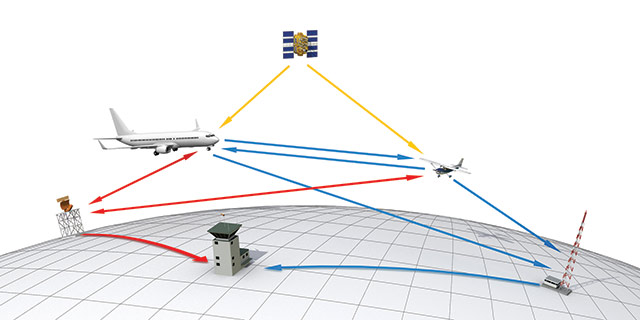
\includegraphics[width=13cm]{pic/Advocacy_ADS_B.jpg}
\caption{ADS-B 系统工作原理\protect\footnotemark}
\label{fig:Advocacy_ADS_B}
\end{figure}

\footnotetext{图片来源:\url{https://www.aopa.org/advocacy/advocacy-briefs/}}

ADS-B 分为两个部分:ADS-B In 和 ADS-B Out。ADS-B In 是系统的接收部分,负责接收 ADS-B 信息;ADS-B Out 是安装有发射器的面板,负责向其他飞机和地面站发送信号,这将告诉其他飞机和地面站本飞行器的位置、速度和航向等信息。注意 ADS-B Out 设备是始终安装在飞机上的并且需要经过认证,这个设备不可拆卸。这样做的目的是为了防止在未授权的情况下,人为关闭 ADS-B 等其他监视跟踪设备,致使无法追踪飞机位置,导致像马来西亚航空 MH370 航班那样的事故。

\subsection{数据链类型}

为了避免频率过载,ADS-B 可以使用不同的数据链以使用不同的频率收/发数据。目前可以支持 ADS-B 技术的数据链主要有三种,分别是基于 S 模式的 \acs{1090ES} 数据链、\acs{978UAT} 数据链和 \acs{VDL Mode4} 数据链。这三种数据链技术各有优缺点,当前美国同时使用 1090ES 和 978UAT 数据链,欧洲同时使用 1090ES 和 VDL Mode4 数据链,而澳大利亚仅使用 1090ES 数据链。目前只有 S 模式 1090ES 数据链获得国际无线电组织的批准,同时国际民航组织对 1090ES 数据链的支持力度最大,标准也最完善。你可以拥有多种 ADS-B 产品:仅 978 In、978 In\&Out、仅 1090ES Out 等等。

\subsubsection{1090ES 数据链}

1090ES 是一个使用扩展震荡信标的改进的 S 模式转发器(使用转发器的 1090MHz 频率),
使用高度要超过 18000 英尺。

\subsubsection{978UAT 数据链}

在美国,18000 英尺以下的高度层使用这种数据链,它在 978MHz 上传输,在技术上称为通用访问收发机。

\subsubsection{VDL Mode4 数据链}

模式 4 甚高频数据链是经 \acs{ICAO} 和 \acs{ETSI} 标准化的甚高频数据链技术,用于提供移动基站(飞行器和机场地面车辆)、移动单元和固定基站之间的数字通信,它的传输频率在 25 kHz\upcite{h8}。

\section{ADS-B 系统的应用意义}

当前世界范围内空中交通流量与密度不断增加,在未来的几十年内,随着无人机的普及,有人驾驶飞机和无人机都需要在同一片空域正常且无冲突地运行。下一代空中交通管理系统是处理空中流量爆发式增长和保证数十亿乘客安全的关键所在。ADS-B 是这一关键的核心技术,它的出现,将大幅提升航行监视系统的态势感知能力。当前我国民航空中监视系统的中流砥柱是二次雷达,这种基于传统通信模式的的监视设备一般可以报告飞机的身份识别代码、高度代码、飞机地址等信息,由于消息长度限制,不能提供位置完整性报告。为了保持空中交通的效率,同时保证安全,需要提供更精确的监测系统和消息的完整性,ADS-B 可以克服当前雷达系统的局限性并提高其监视性能,增加空域容量,在无法部署雷达的内陆地区,ADS-B 能为飞机提供优于雷达间隔标准的虚拟雷达管制服务;在有雷达覆盖地区,在不增加雷达设备的情况下,能够以较低代价辅助现有雷达系统。ADS-B 系统并非一个独立的监视系统,它对外部系统的高度依赖,比如 \acs{GPS} 系统将为其提供位置报告,正因为此,ADS-B 的监视精度可以提高至 10 米量级,监视数据更新速度可达 1 秒 1 次。另外,ADS-B 技术成本较低,其地面站建设成本是传统二次雷达的九分之一。ADS-B 技术将为传统空管监视领域带来重大变革。

\section{ADS-B 系统的发展现状}

国际民航组织于第十一届航行大会确定 ADS-B 技术为全球新航行技术的主要发展方向,目前全球各国都在不懈推广 ADS-B 技术的应用。目前对 ADS-B Out 进行强制装备或建议装备的国家越来越多\upcite{h7},部分有 ADS-B Out 装备要求和建议的国家见表\ref{tab:Countries_with_ADS-B_Out_mandates_and_proposals}。

\renewcommand\arraystretch{1.5}
\begin{table}[!htb]
\centering
\caption{部分有 ADS-B Out 装备要求和建议的国家\protect\footnotemark}
\label{tab:Countries_with_ADS-B_Out_mandates_and_proposals}
\begin{tabular}[b]{|p{2cm}<{\raggedleft}|p{13cm}<{\raggedright}|}
\hline
\textbf{美国} & 美国联邦航空局已要求在 2020 年 1 月 1 日之后所有飞机需要装备 ADS-B Out,目前大部分空域需要装备 C 模式转发器。有一个重要的例外情况:在墨西哥湾以上的某个空域也需要 ADS-B。目前,只有美国允许将 978UAT 数据链路用于 ADS-B Out。如果计划在美国以外的 ADS-B 空域飞行,则需要使用 S 模式 1090ES 数据链路 \\
\hline
\textbf{澳大利亚} & 所有 \acs{IFR} 飞行都需要 1090ES。2020 年 6 月 6 日之前,配备转发器的外国注册飞机在飞行高度低于 \acs{FL}290 时免于装备 1090ES \\
\hline
\textbf{加拿大} & 目前没有要求,但自愿装备 1090ES(特别是在哈德逊湾和附近的海洋空域)的运营商可以获得更高水平的服务。NAV CANADA 是 Aireon 联合空中交通监控机构的一部分,在低地球轨道卫星上安装 ADS-B 设备。NAV CANADA 将在 2018 年提供服务时成为启动客户,并且最初打算将 1090ES ADS-B 纳入北大西洋空域 \\
\hline
\textbf{欧洲} & \acs{MTOW} 超过 12566 磅,或最大巡航空速超过 250 节的 IFR 飞机需要装备 1090ES,对于新生产的飞机要求强制装备,并且必须在 2020 年 6 月 7 日之前对所有飞机进行改装 \\
\hline
\textbf{香港} & 所有空域 FL290 及以上需要 1090ES \\
\hline
\textbf{印度尼西亚} & FL290 及以上需要 1090ES \\
\hline
\textbf{墨西哥} & 从 2020 年 1 月 1 日开始,在平均海平面 10000 英尺以上 A、B、C、E 级空域以及其他指定的空域需要 1090ES;目前要求在墨西哥湾的 E 级空域和墨西哥海岸 12 海里以内平均海平面 3000 英尺以上需要 1090ES \\
\hline
\textbf{新加坡} & 指定的航空公司需要 1090ES \\
\hline
\textbf{斯里兰卡} & Colombo 的 \acs{TMA},FL290 及以上需要需要 1090ES \\
\hline
\textbf{台湾} & 所有空域 FL290 及以上需要 1090ES \\
\hline
\textbf{越南} & 指定的航空公司需要 1090ES \\
\hline
\end{tabular}
\end{table}

\footnotetext{数据来源:\url{https://www.aopa.org/go-fly/aircraft-and-ownership/ads-b/where-is-ads-b-out-required}}

\subsection{国外应用现状}

目前欧美等航空发达国家已制定本国和本地区的 ADS-B 实施规划,建立相关的规章和标准,开展验证与应用。

\subsubsection{北美地区}

在国外,美国是最先开展 ADS-B 技术研究和应用的国家之一,是美国 NextGen 计划的基础之一,帮助飞行员和空中交通管制员创建一个更安全、更高效的 NAS。美国的 ADS-B 应用路线是:先通用航空,后商用运输。目前,在通用航空方面,美国已经完全实现使用 ADS-B 技术来为自己的航空器提供监视服务。

2016 年 9 月,\acs{FAA} 开始提供 500 美元奖励,以帮助通用航空运营商支付 ADS-B 设备和安装费用,并鼓励他们现在就装备。

FAA 要求在 2020 年之前,所有在受控空域飞行的飞机都必须安装有 ADS-B OUT,而对 ADS-B In 的安装没有强制要求。

2016 年,FAA 与墨西哥的空中交通服务提供商 SENEAM 合作,使用合资建立的 ADS-B 地面站扩展在墨西哥湾上空的 ADS-B 监视覆盖水平。新的地面站有助于飞行器飞过美国和墨西哥之间的墨西哥湾。

墨西哥的其他地面站对于空中交通路线提供无缝监控覆盖,使海湾地区的容量从每小时 75 架增加到约 85 架。到 2035 年,这些地面站将为美国-墨西哥领空边界提供更多的海湾航班,从而为运营商节省 7000 万美元。增加容量可减少高峰期的延误,从而节省飞机运营成本和乘客时间。

FAA 正在开发 Interval Management,这是一套借助 ADS-B 的能力对航班进行排队和分配的应用软件。间隔管理的精确间距可以在拥挤的空域内实现更高效的飞行路径,并最大限度地提高空域和机场利用率。这些功能需要新的航空电子设备、地面自动化、决策支持系统和程序。FAA 也在探索 ADS-B 在越来越多的商用太空飞行器发射方面的能力。FAA 也在和运营商和其他的 \acs{ANSP} 合作,以评估向海洋空域的管制方提供 ADS-B 数据潜在利益。减少分离标准的替代方法包括使用 ADS-B 或使用增强版本 \acs{ADS-C}。

\subsubsection{澳大利亚}

澳大利亚的 ADS-B 应用水平也达到了很高的程度,该国地广人稀,雷达监视系统建设部署比较薄弱,鉴于这种情况,澳大利亚开始投资部署 ADS-B 系统以配合为数不多的航管雷达设备。

\subsubsection{欧洲}

欧洲各国 ADS-B 应用水平也在大力推进,当前位于欧洲中部的 OpenSky 感知网络的 ADS-B 系统可以捕捉到欧洲大约 30\% 的商业航班,其监视能力相当可观。ADS-B 也是 SESAR 的基石,欧盟(欧洲共同体和欧控)是 SESAR 的创始人。

欧洲 ADS-B 实施计划要求从 2015 年起,质量大于 5700kg 或速度超过 250 节的新飞行器当在以 IFR 下飞行时要装备 ADS-B Out,已经运营的飞机从 2017 年底开始进行改装,在 2020 年 ADS-B 监视系统需要开始运作\upcite{h2}。

\subsection{国内应用现状}

在 ADS-B 技术的研发应用方面,中国民航紧跟国际发展动态,努力与世界接轨。当今 ADS-B 监视技术已在中国民航处于实用阶段,截至 2014 年底,中国民航全行业运输飞机注册架数已达 2370 架,部分已完成 1090ES ADS-B OUT 机载设备加改装。中国民航在西部高原地区实施了 B213 航路(成都-拉萨)ADS-B 试验工程和试验运行,并缩小了航路间隔;在 B330 成都-九寨航路、南中国海开展了 ADS-B 试验验证工作。2015 年,中国民用航空 ADS-B 实施规划颁布,是指导中国民航 ADS-B 实施的纲领性文件。

\subsection{技术发展现状}

在硬件设备的发展上,由于 ADS-B 非独立监视的特性,就像接收广播一样,只要找到合适的设备,用户就可以通过各种渠道接收 ADS-B 信号,由于其技术门槛与
成本相对较低,所以 ADS-B 技术目前被广泛推广。在硬件方面,虽然商用 ADS-B 接收器比较昂贵,但是相较于雷达这种高度精密的设备,其成本也大大降低了。事实上,目前通过一些廉价的接收设备,比如数字电视棒,也可以接收 ADS-B 信号。国内外许多厂家也推出了廉价的 ADS-B 接收设备,例如 RTL-SDR、AirNav RadarBox、三航雷达等。目前国内在民航局政策与标准引导下,工业界已基本具备 ADS-B 设备产业化能力。

\section{全球 ADS-B 覆盖情况}

本小节将介绍世界上几个典型的国家和地区的 ADS-B 实施情况。

\subsection{全球}

全球 ADS-B 覆盖情况如图\ref{fig:1ADS-B-coverage}所示。

\begin{figure}[!htb]
\centering
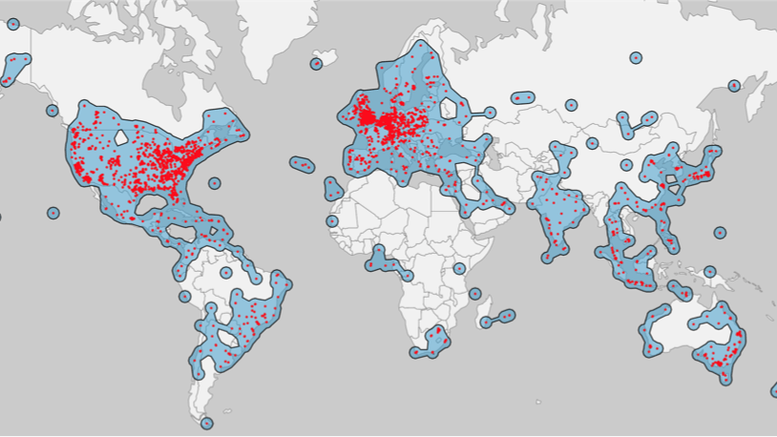
\includegraphics[width=14cm]{pic/1ADS-B-coverage.png}
\caption{全球陆基 ADS-B 覆盖情况\protect\footnotemark}
\label{fig:1ADS-B-coverage}
\end{figure}

\footnotetext{图片来源:\url{https://jdasolutions.aero/blog/ads-b-update-bits-information-around-world/}}

\subsection{澳大利亚}

ADS-B 地面站是 LOS \footnote{通常指波的传播路径为直线,不能沿曲线或者跨障碍物行进}设施,地面站接收下行 ADS-B 数据的能力取决于飞机的高度、飞机与地面站的距离以及障碍物。在海拔较低的低空区域(接近地面),覆盖范围在距离地面站 20 海里半径内,高空空域覆盖半径可以超过 250 海里。

在雷达覆盖范围与 ADS-B 覆盖范围重叠的空域,雷达探测到的飞机位置将会提交给 \acs{ATC}。

截至 2017 年 1 月,澳大利亚纯 ADS-B 覆盖区域如图\ref{fig:ADS-B-5000}、\ref{fig:ADS-B-10k}、\ref{fig:ADS-B-20k}、\ref{fig:ADS-B-30k}所示,澳大利亚 30000 英尺以上高空已实现 ADS-B 密集覆盖,航路管制间隔已缩至 5 海里水平。

\begin{figure}[!htb]
\centering
\begin{minipage}[t]{0.48\textwidth}
\centering
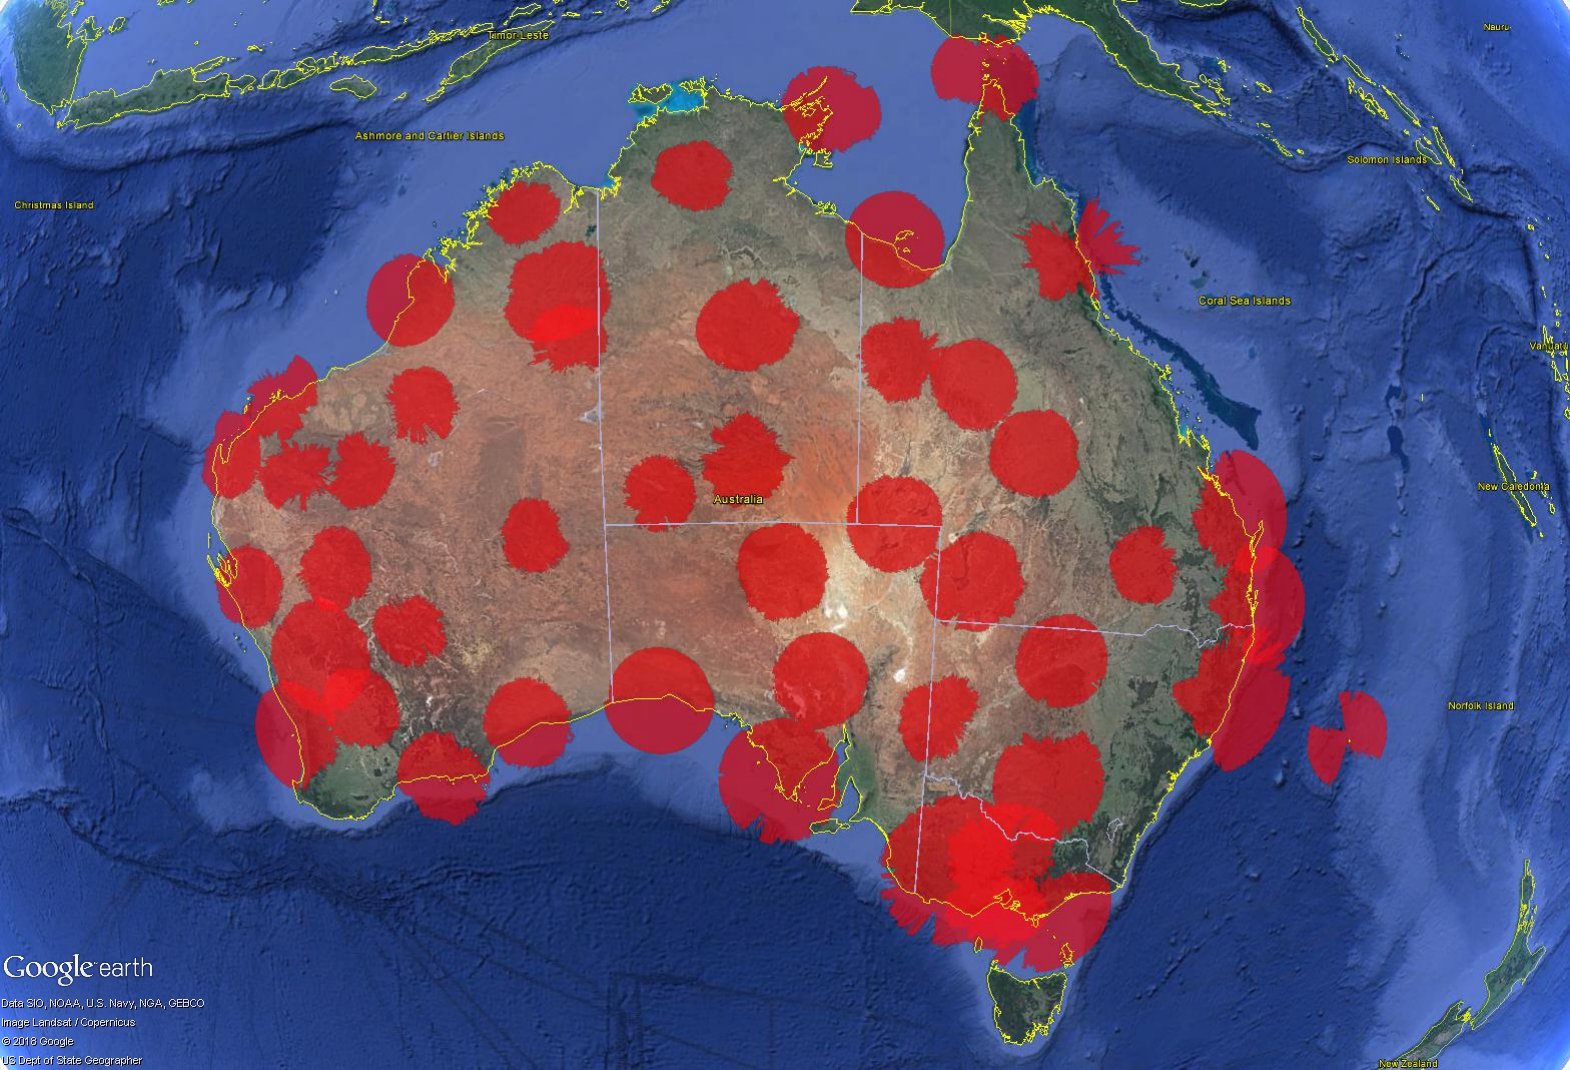
\includegraphics[width=7.5cm]{pic/ADS-B-5000.jpg}
\caption{澳洲 5000ft 空域覆盖范围\protect\footnotemark}
\label{fig:ADS-B-5000}\footnotetext{图片来源:\url{http://www.airservicesaustralia.com/projects/ads-b/ads-b-coverage/}}
\end{minipage}
\begin{minipage}[t]{0.48\textwidth}
\centering
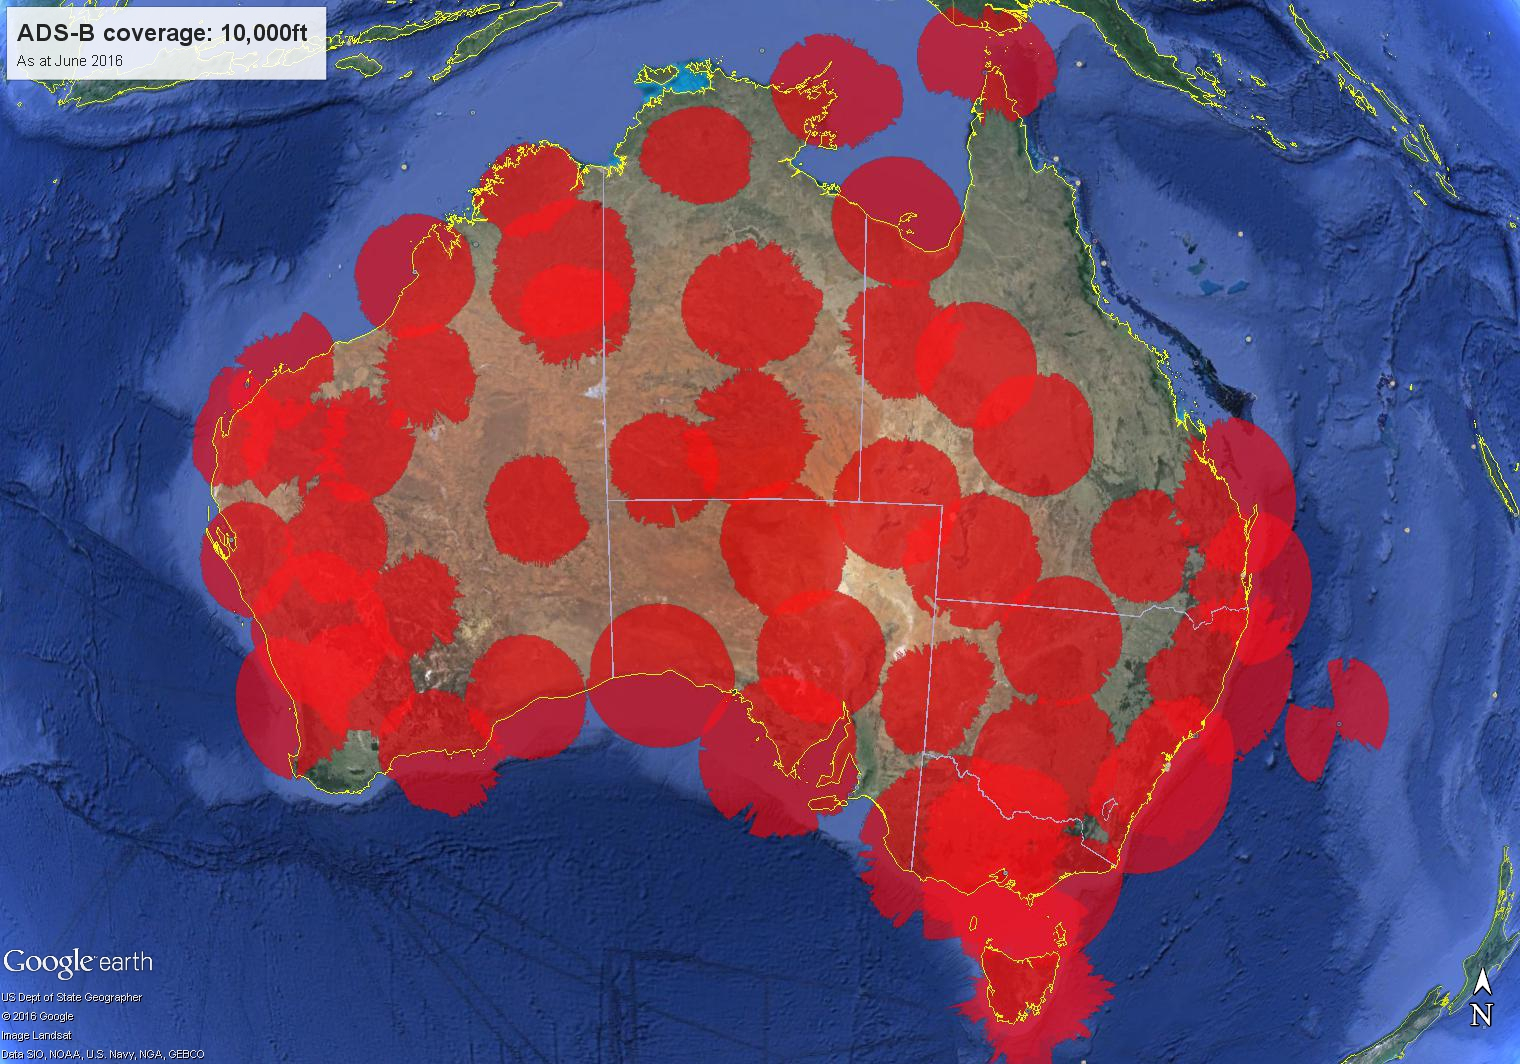
\includegraphics[width=7.5cm]{pic/ADS-B-10k.jpg}
\caption{澳洲 10000ft 空域覆盖范围\protect\footnotemark}
\label{fig:ADS-B-10k}\footnotetext{图片来源:\url{http://www.airservicesaustralia.com/projects/ads-b/ads-b-coverage/}}
\end{minipage}
\end{figure}

\begin{figure}[!htb]
\centering
\begin{minipage}[t]{0.48\textwidth}
\centering
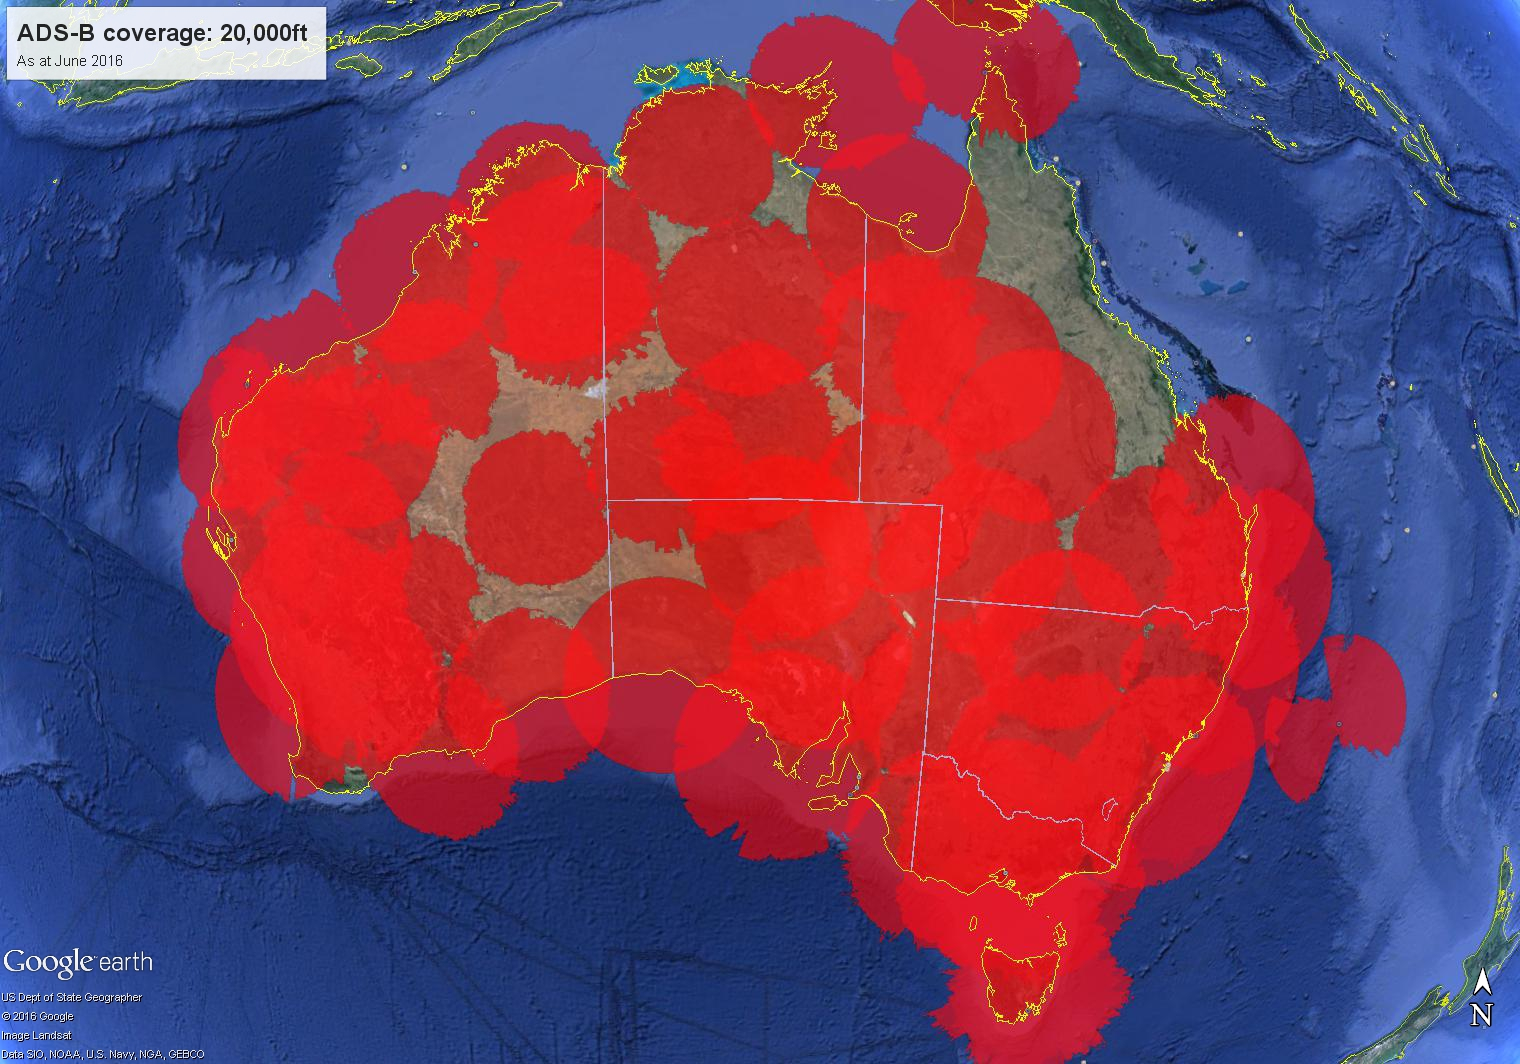
\includegraphics[width=7.5cm]{pic/ADS-B-20k.jpg}
\caption{澳洲 20000ft 空域覆盖范围\protect\footnotemark}
\label{fig:ADS-B-20k}\footnotetext{图片来源:\url{http://www.airservicesaustralia.com/projects/ads-b/ads-b-coverage/}}
\end{minipage}
\begin{minipage}[t]{0.48\textwidth}
\centering
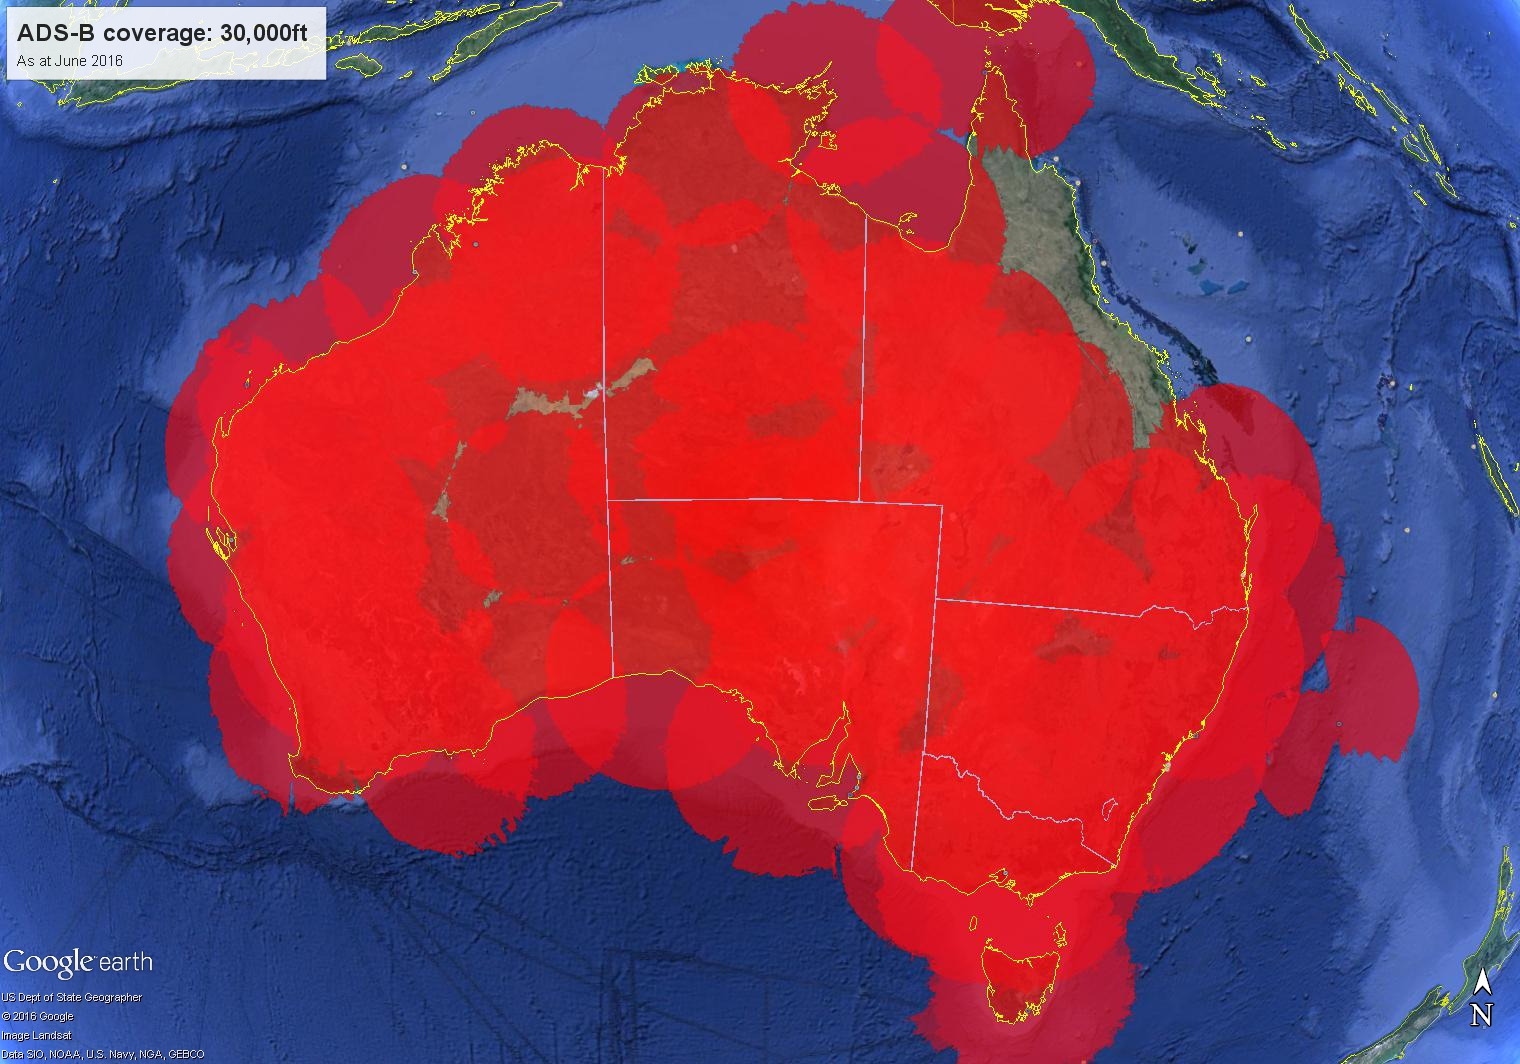
\includegraphics[width=7.5cm]{pic/ADS-B-30k.jpg}
\caption{澳洲 30000ft 空域覆盖范围\protect\footnotemark}
\label{fig:ADS-B-30k}\footnotetext{图片来源:\url{http://www.airservicesaustralia.com/projects/ads-b/ads-b-coverage/}}
\end{minipage}
\end{figure}

\subsection{北美地区}

截至 2017 年 4 月,ADS-B 在美国全境的覆盖情况如图\ref{fig:ADS-B-Coverage-Area}所示。

\begin{figure}[!htb]
\centering
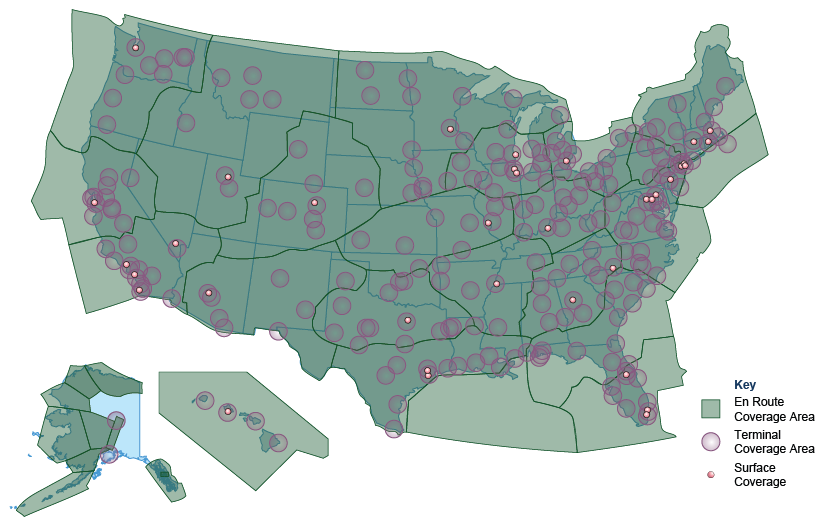
\includegraphics[width=14cm]{pic/ADS-B-Coverage-Area.png}
\caption{美国陆基 ADS-B 覆盖情况\protect\footnotemark}
\label{fig:ADS-B-Coverage-Area}
\end{figure}

\footnotetext{图片来源:Corporate Fleet Service(CFS),\url{http://cfsjets.com/2017/12/14/ads-b-where-we-are-now//}}

根据美国麻省理工学院 2011 年 6月的一份报告\upcite{e3}显示,预计 ADS-B 在美国全面实施后其覆盖情况如图\ref{fig:ADSB-final}所示。

\begin{figure}[!htb]
\centering
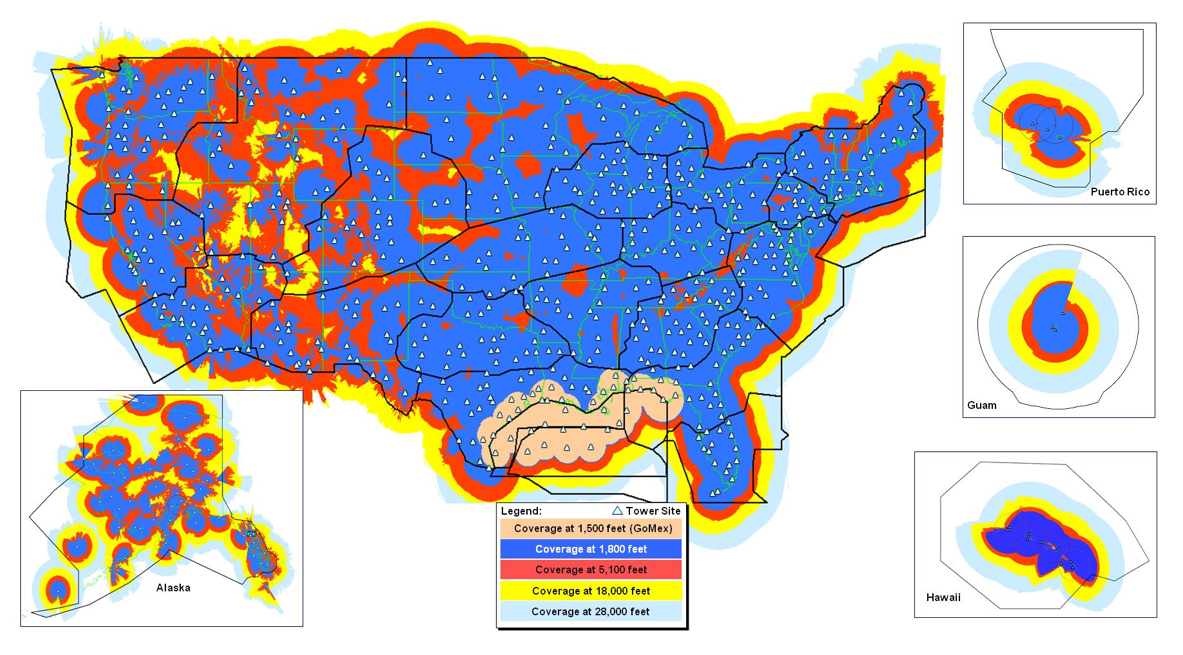
\includegraphics[width=14cm]{pic/ADSB-final.png}
\caption{预测的 ADS-B 全面实施后的覆盖率\protect\footnotemark}
\label{fig:ADSB-final}
\end{figure}

\footnotetext{图片来源:参考文献\cite{e3,e4}}

更为详细的 ADS-B 覆盖情况可以在 FAA 网站\footnote{\url{https://www.faa.gov/nextgen/programs/adsb/}}上查询,它提供了一个动态的可交互式的 ADS-B 覆盖范围查询网页。

\subsection{欧洲}

\subsubsection{现阶段}

\begin{itemize}

    \item \textbf{地面段 ADS-B(基站部署)- 空域和机场监视}

    2018 年 5 月 15 日的 SESAR 关于欧洲 ADS-B 系统建设的阶段性报告展示了欧洲 ADS-B 系统的相关情况\upcite{e5}。

    图\ref{fig:20180515-sesar-ads-b-report_18}显示了欧洲 ADS-B 监控系统的实施现状、相关覆盖范围,以及 \acs{ATM} 系统中相关监控数据的集成水平。

    \begin{figure}[!htb]
    \centering
    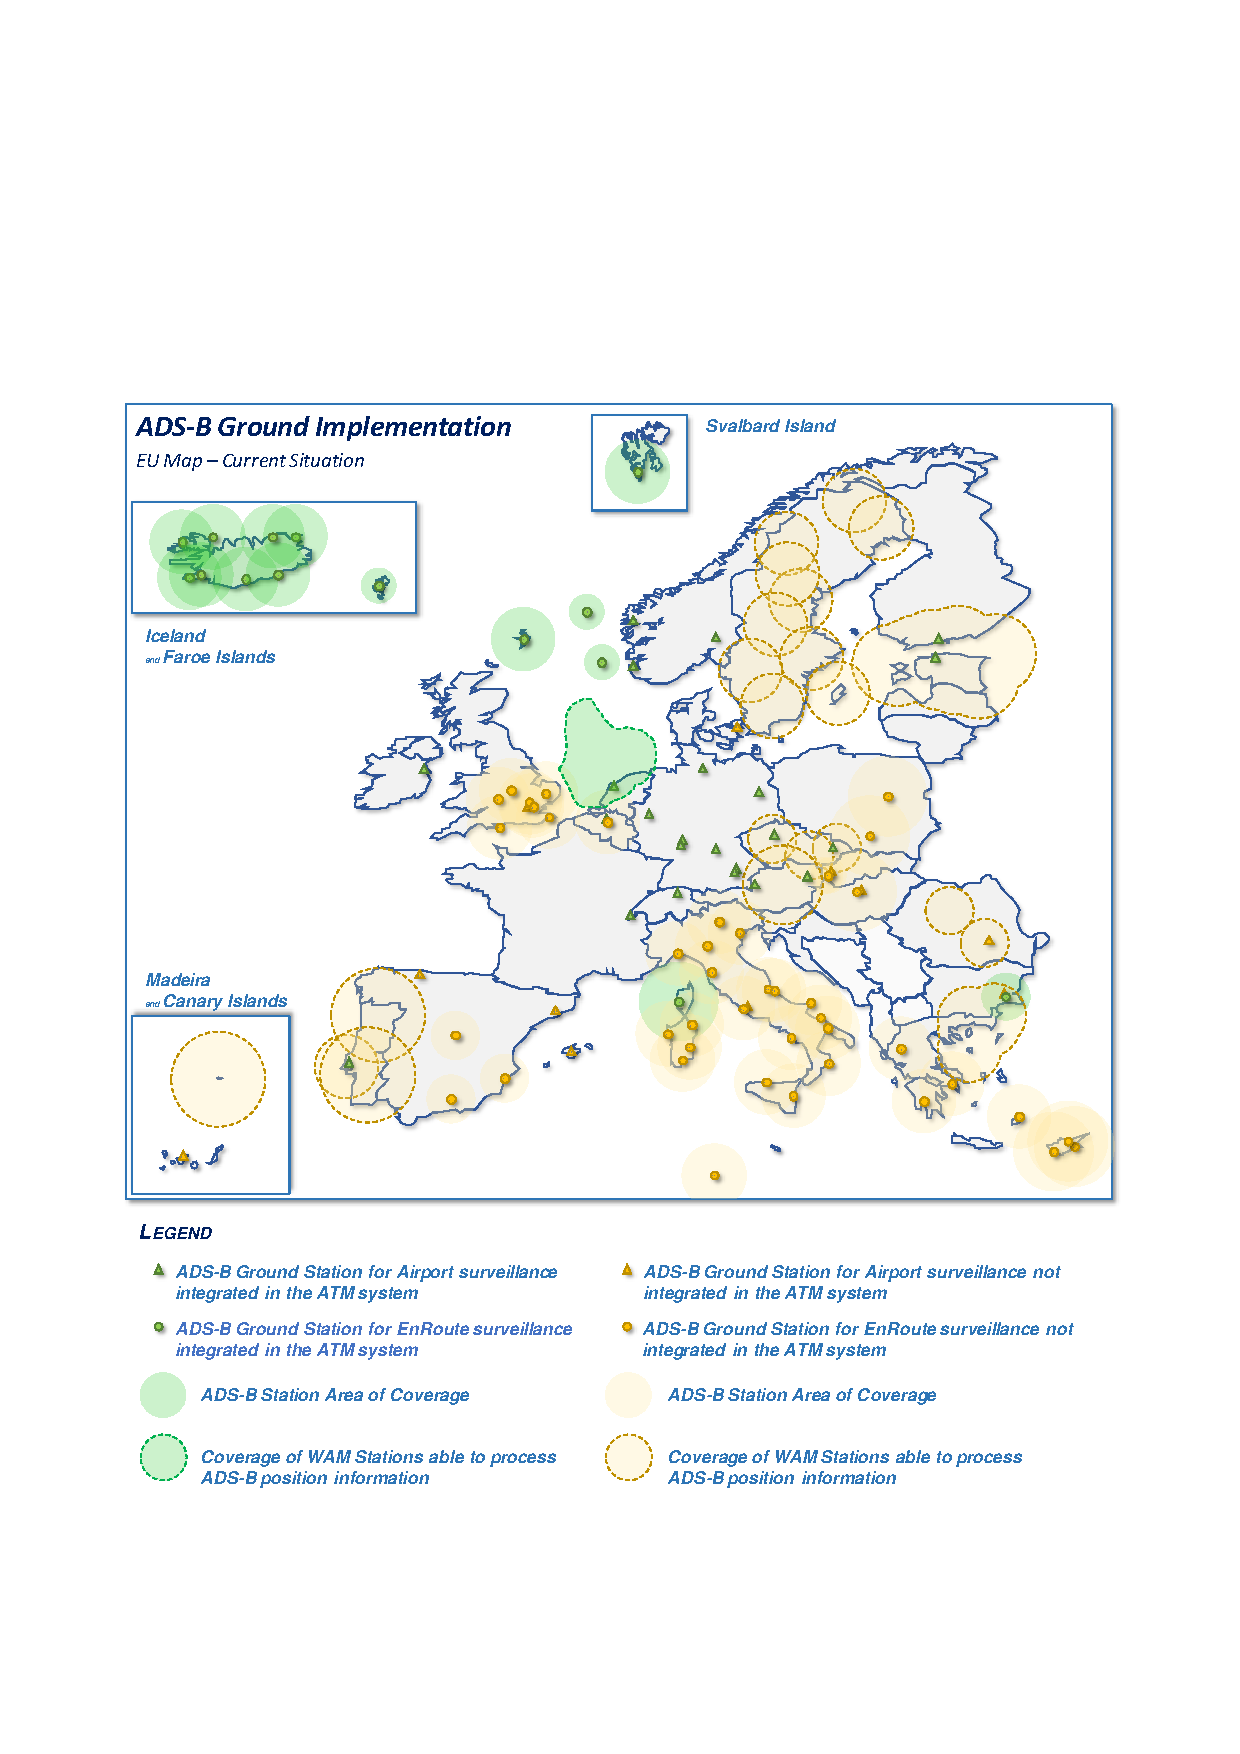
\includegraphics[width=14cm]{pic/20180515-sesar-ads-b-report_18.pdf}
    \caption{欧洲 ADS-B 地面监控系统的实施现状\protect\footnotemark}
    \label{fig:20180515-sesar-ads-b-report_18}
    \end{figure}

    \footnotetext{图片来源:参考文献\cite{e5}}

    \begin{itemize}
        \item \textbf{空域 ADS-B 监视}

        欧洲 ADS-B 接收机的安装现状比较零散。总共安装了 70 多个具备航路 ADS-B 监控能力的基站,其中约 90\% 在运行中,其余 10\% 用于测试和验证。现有 ADS-B 站的剩余平均寿命为 12 年。

        \item \textbf{机场 ADS-B 监视}

        用于机场监控的 ADS-B 系统非常广泛,目前,欧洲共安装了 34 个机场 ADS-B 站:其中 23 个被集成到 ATM 系统中,11 个没有被集成到 ATM 系统中,但计划将它们与 \acs{MLAT} 系统集成。机场 ADS-B 在与 ATM 系统集成时,无论是否与 MLAT 结合,都只用于地面车辆的识别和定位数据,因为数据质量要求没有飞机那么严格。现有 ADS-B 站的剩余平均寿命为 8 年。
    \end{itemize}

    \item \textbf{空中段 ADS-B(机上终端)}

    图\ref{fig:airborne-ads-b-euro}显示了符合 ADS-B ED-102A(DO-260B)规定的 ADS-B 应答器的实施现状,该应答器共装备于 35 家总部位于欧盟的航空公司的共 3108 架飞机上。

    \begin{figure}[!htb]
    \centering
    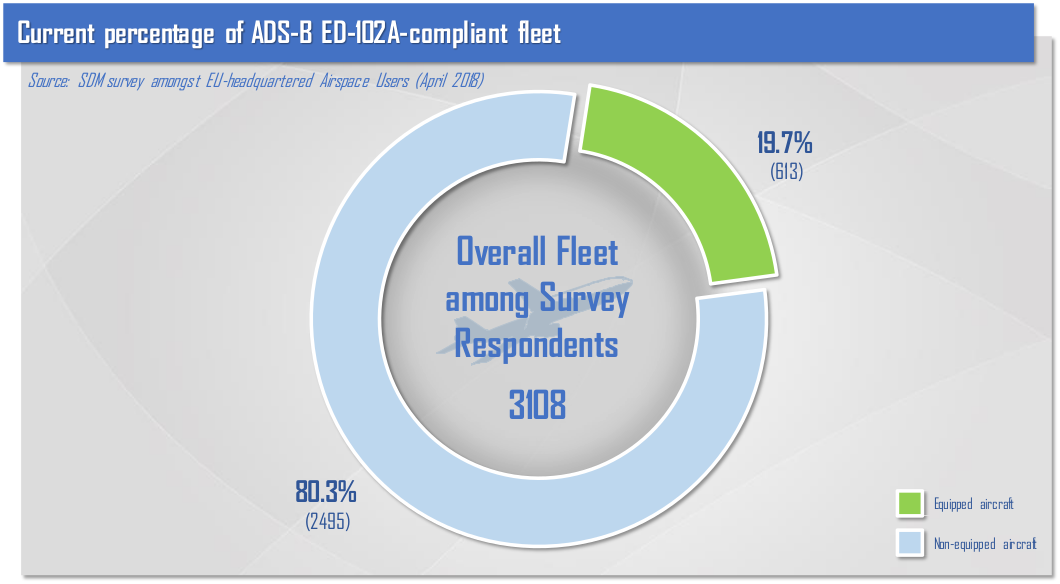
\includegraphics[width=16cm]{pic/airborne-ads-b-euro.png}
    \caption{欧洲各国现阶段飞机 ADS-B 终端装备情况\protect\footnotemark}
    \label{fig:airborne-ads-b-euro}
    \end{figure}

    \footnotetext{图片来源:参考文献\cite{e5}}

    \item \textbf{星基 ADS-B}

    关于星基 ADS-B 信息的地面使用情况,28 家 ANSP 在回答问卷时表示,15 家 ANSP 没有使用星基 ADS-B 数据的计划,而 13 家 ANSP 表示,一旦服务可用,他们正在考虑使用该数据。

    \acs{NATS} 和 NAV CANADA 计划在 2019-2020 年期间在北大西洋和加拿大部署星基 ADS-B (Aireon)。一些欧洲的 ANSP 计划从 2019 年第一季度开始使用它。

\end{itemize}

\subsubsection{2020 年及以后}

\begin{itemize}

    \item \textbf{2020 年地面段 ADS-B(基站部署)- 空域和机场监视}

    图\ref{fig:20180515-sesar-ads-b-report_33}显示了利益攸关方在全欧洲实施 ADS-B 监控系统的短期计划。特别是,该图包括所有预计在 2020 年之前安装和/或运行的 ADS-B 系统。

    \begin{figure}[!htb]
    \centering
    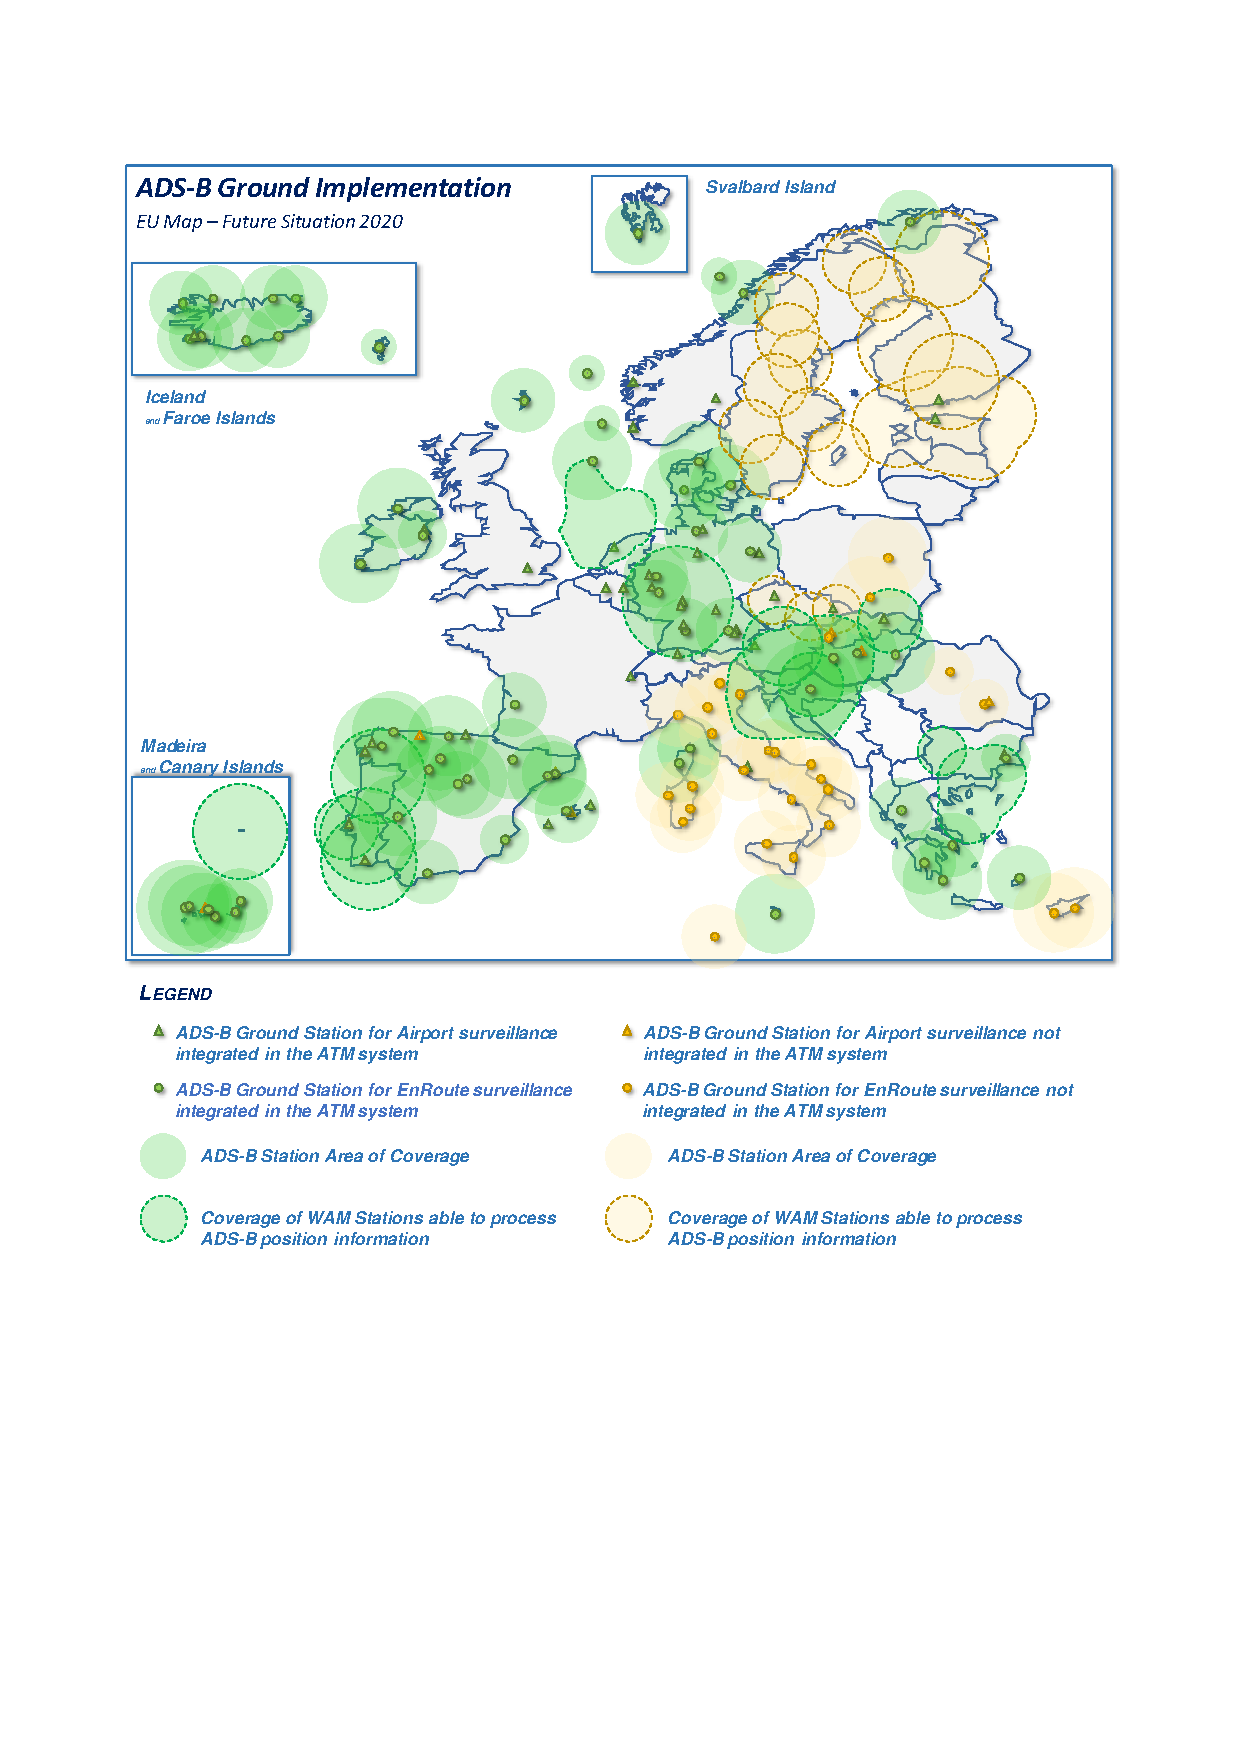
\includegraphics[width=15cm]{pic/20180515-sesar-ads-b-report_33.pdf}
    \caption{欧洲 2020 年 ADS-B 地面监控系统实施计划\protect\footnotemark}
    \label{fig:20180515-sesar-ads-b-report_33}
    \end{figure}

    \footnotetext{图片来源:参考文献\cite{e5}}

    \begin{itemize}
        \item \textbf{空域 ADS-B 监视}

        未来欧洲 ADS-B 接收机的安装情况显示,采用 ADS-B 的趋势越来越明显。在 ANSP 的投资计划中,总共有 60 多个具备 ADS-B 能力的航路监测站。值得强调的是,由 \acs{WAM} 或 ADS-B 基站顶部的 S 模式雷达将提供大量计划中的 ADS-B 功能。

        ADS-B 基站的典型寿命为 15-18 年。

        \item \textbf{机场 ADS-B 监视}

        作为上述投资的补充,ANSP 和机场运营商计划在 2018 年至 2020 年间安装/更新大约 25 个 ADS-B 站,用于机场监控。这些监测站将补充和/或取代现有的基础设施,并将扩大 ADS-B 在欧洲机场的覆盖范围。

        在短期内,ADS-B 基础设施将继续集成到 ATM 系统中,首先跟踪车辆的位置,然后将其增强到飞机上。从 2018 年起,现有 ADS-B 站的剩余平均寿命为 15 年。
    \end{itemize}

    \item \textbf{2020 年以后地面段 ADS-B(基站部署)- 空域和机场监视}

    图\ref{fig:20180515-sesar-ads-b-report_35}补充了前一段展示的短期规划,包括业务利益相关者在未来数年实施 ADS-B 监测系统的长期计划。特别地,该图包括了所有 ADS-B 系统,预计从 2021 年开始安装和运行。

    \begin{figure}[!htb]
    \centering
    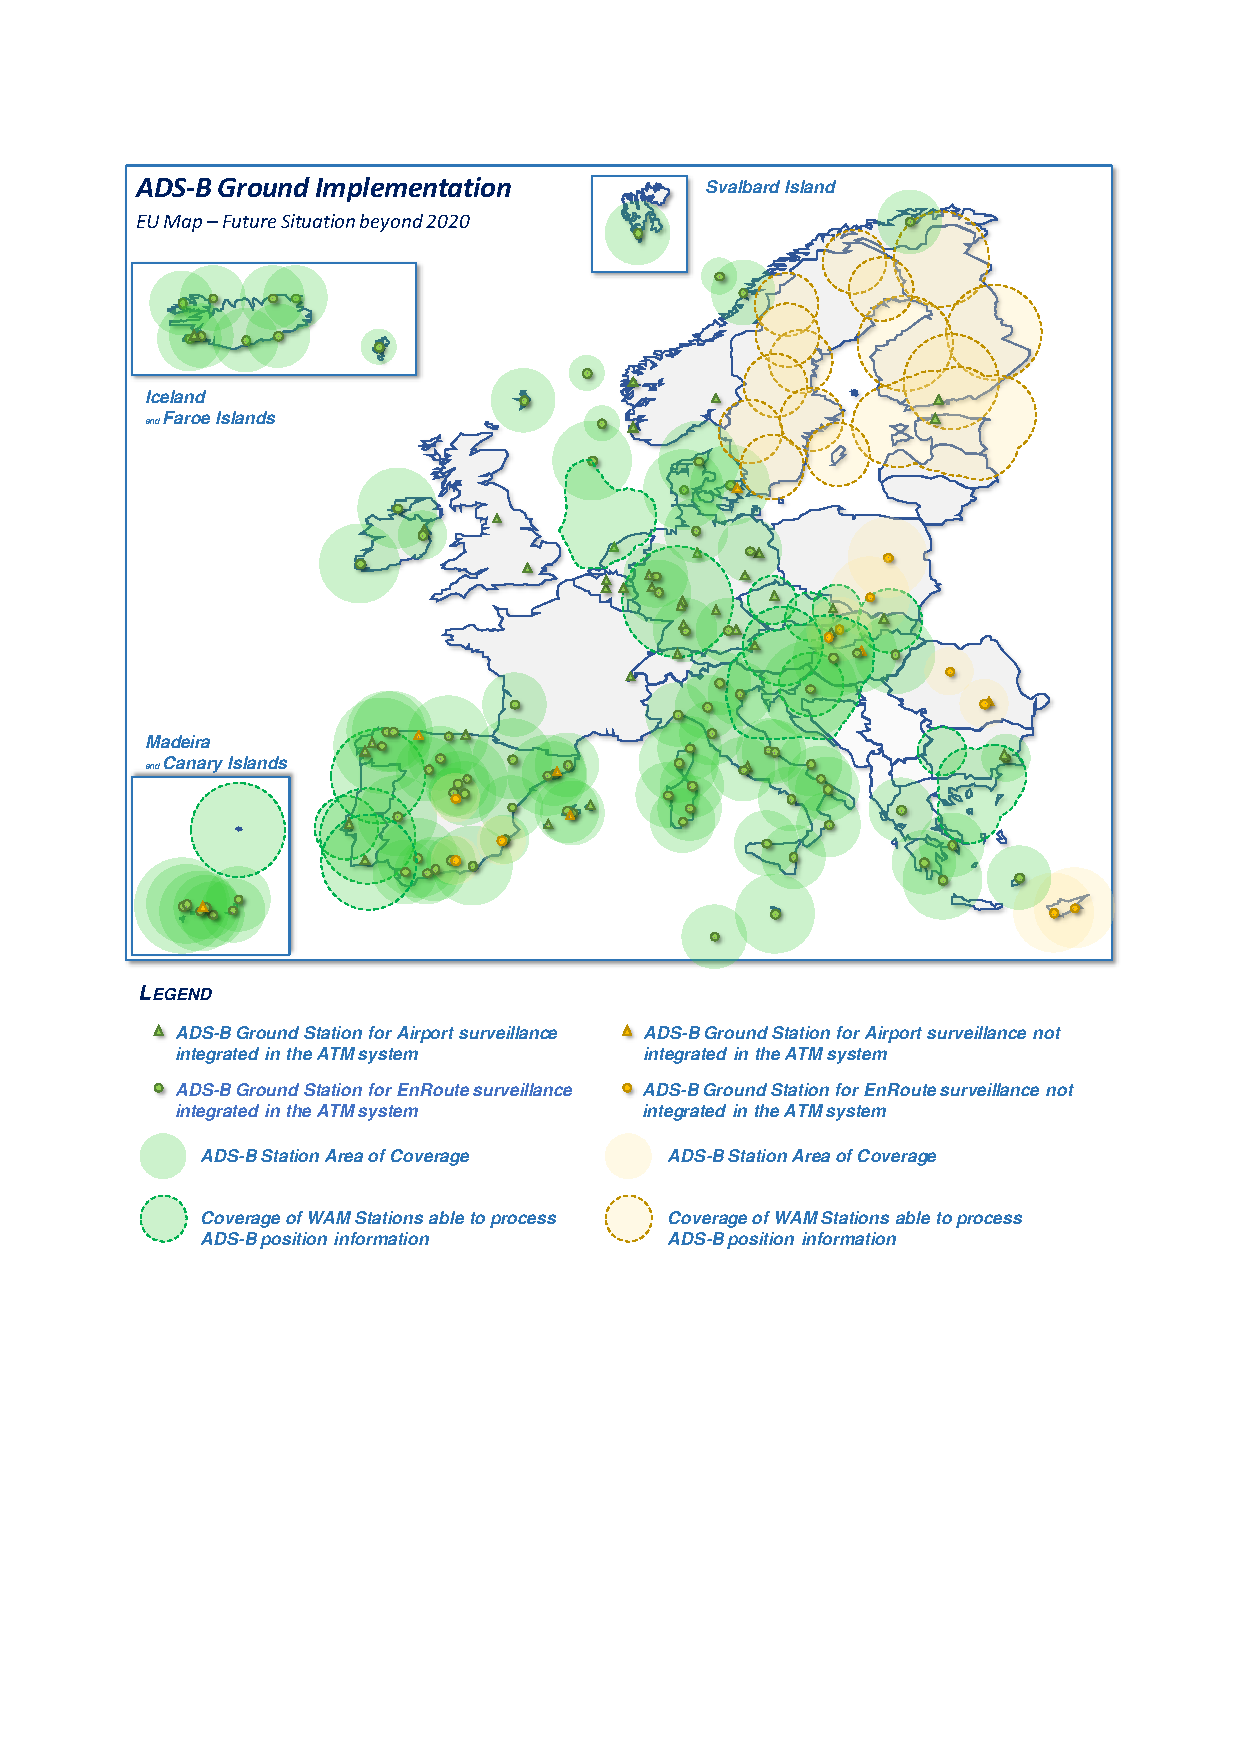
\includegraphics[width=15cm]{pic/20180515-sesar-ads-b-report_35.pdf}
    \caption{欧洲 2020 年之后 ADS-B 地面监控系统实施计划\protect\footnotemark}
    \label{fig:20180515-sesar-ads-b-report_35}
    \end{figure}

    \footnotetext{图片来源:参考文献\cite{e5}}

    \begin{itemize}
        \item \textbf{空域 ADS-B 监视}

        与 2020 年的情况相比,欧洲的 ADS-B 前景略有改善,计划在航线上安装几个具有 ADS-B 能力的监测站。

        西班牙计划增加新的 ADS-B 站,覆盖南部空域(通过在新安装的 S 模式雷达内集成 ADS-B 接收器)。另一方面,意大利和捷克共和国将在业务上使用 ADS-B 数据,从而将信息集成到 ATM 系统中。最后,一个能够接收 ADS-B 数据的额外 WAM 站将覆盖芬兰东部领空,但是没有将这些信息纳入 ATM 系统。

        \item \textbf{机场 ADS-B 监视}

        为配合上述情况,机场服务供应商及机场运营商计划于 2021 年至 2030 年期间安装/更新 6 个 ADS-B 监测站,进行机场监察。这些监测站将补充和/或取代现有的基础设施,并将扩大 ADS-B 在欧洲的覆盖范围。从2018年起,现有 ADS-B 站的剩余平均寿命为 16 年。
    \end{itemize}

    \item \textbf{空中段 ADS-B(机上终端)}

    在未来,各主要航空公司正计划顺应规定对新飞机安装 ADS-B,而对现有飞机进行“翻新计划”的情况则有所不同。欧盟可能决定将 2020 年至 2025 年的过渡期延长 5 年,并进一步豁免 2025 年之前退役的飞机,由此引发的预期进一步放大了这一设想,导致该法规再次修订。

    除欧盟和美国外,ADS-B Out(DO-260B应答器)在中国、澳大利亚或日本等其他国家也有或将被授权使用。

    \item \textbf{星基 ADS-B}

    一些 ANSP 正在考虑基于 ADS-B 的空间服务,并且正在进行调查(基于 Aireon 的服务可用性)。三家 ANSP 正计划使用基于空间的 ADS-B。在意大利,星基 ADS-B 系统将集成在 \acs{ATS} 测试平台上,预计 2020 年后的业务用途将作为地面独立的 ATS 监视层,用于应急和增强监视。中期而言,这可能是传统监控基础设施全球优化的一部分。

\end{itemize}

\subsection{中国}

根据 ICAO 第十五次 ADS-B 研究和实施研讨会(ADS-B SIFT/15)议信息论文(IP,Information Paper)IP/31 \upcite{e6}显示,\acs{CAAC} 于 2015 年 12 月修订了《中国民用航空 ADS-B 实施方案》。根据国家 ADS-B 建设项目审批及实施进度,主要修改是调整各阶段的实现时间。

\begin{itemize}
    \item \textbf{第一阶段}:2017 年底,ADS-B 在中国开始初步运营,以及在 ATS 路线上实施 ADS-B :B213、B345、B215、A460、H66、L888、H15、Z1、B206、A368、M771、L642、N892 和 A1。

    \item \textbf{第二阶段}:2017 年至 2020 年,重点任务是全面推进 ADS-B Out,并对 ADS-B Out 进行安全评估。

    \item \textbf{第三阶段}:2020 年至 2025 年,建成完善的 ADS-B 运营监控系统和信息服务系统,为航空公司提供全空域监控手段和综合 ADS-B 信息服务,增强空中交通管制安全保障能力和服务水平。
\end{itemize}

2017 年底(阶段一)将部署 310 个 ADS-B 地面站、2 个 ADS-B 主数据处理中心、8 个 ADS-B 次数据处理中心。本阶段全国 ADS-B 覆盖率如图\ref{fig:china_3300m}、\ref{fig:china_6600m}、\ref{fig:china_8400m}所示。

\begin{figure}[!htb]
\centering
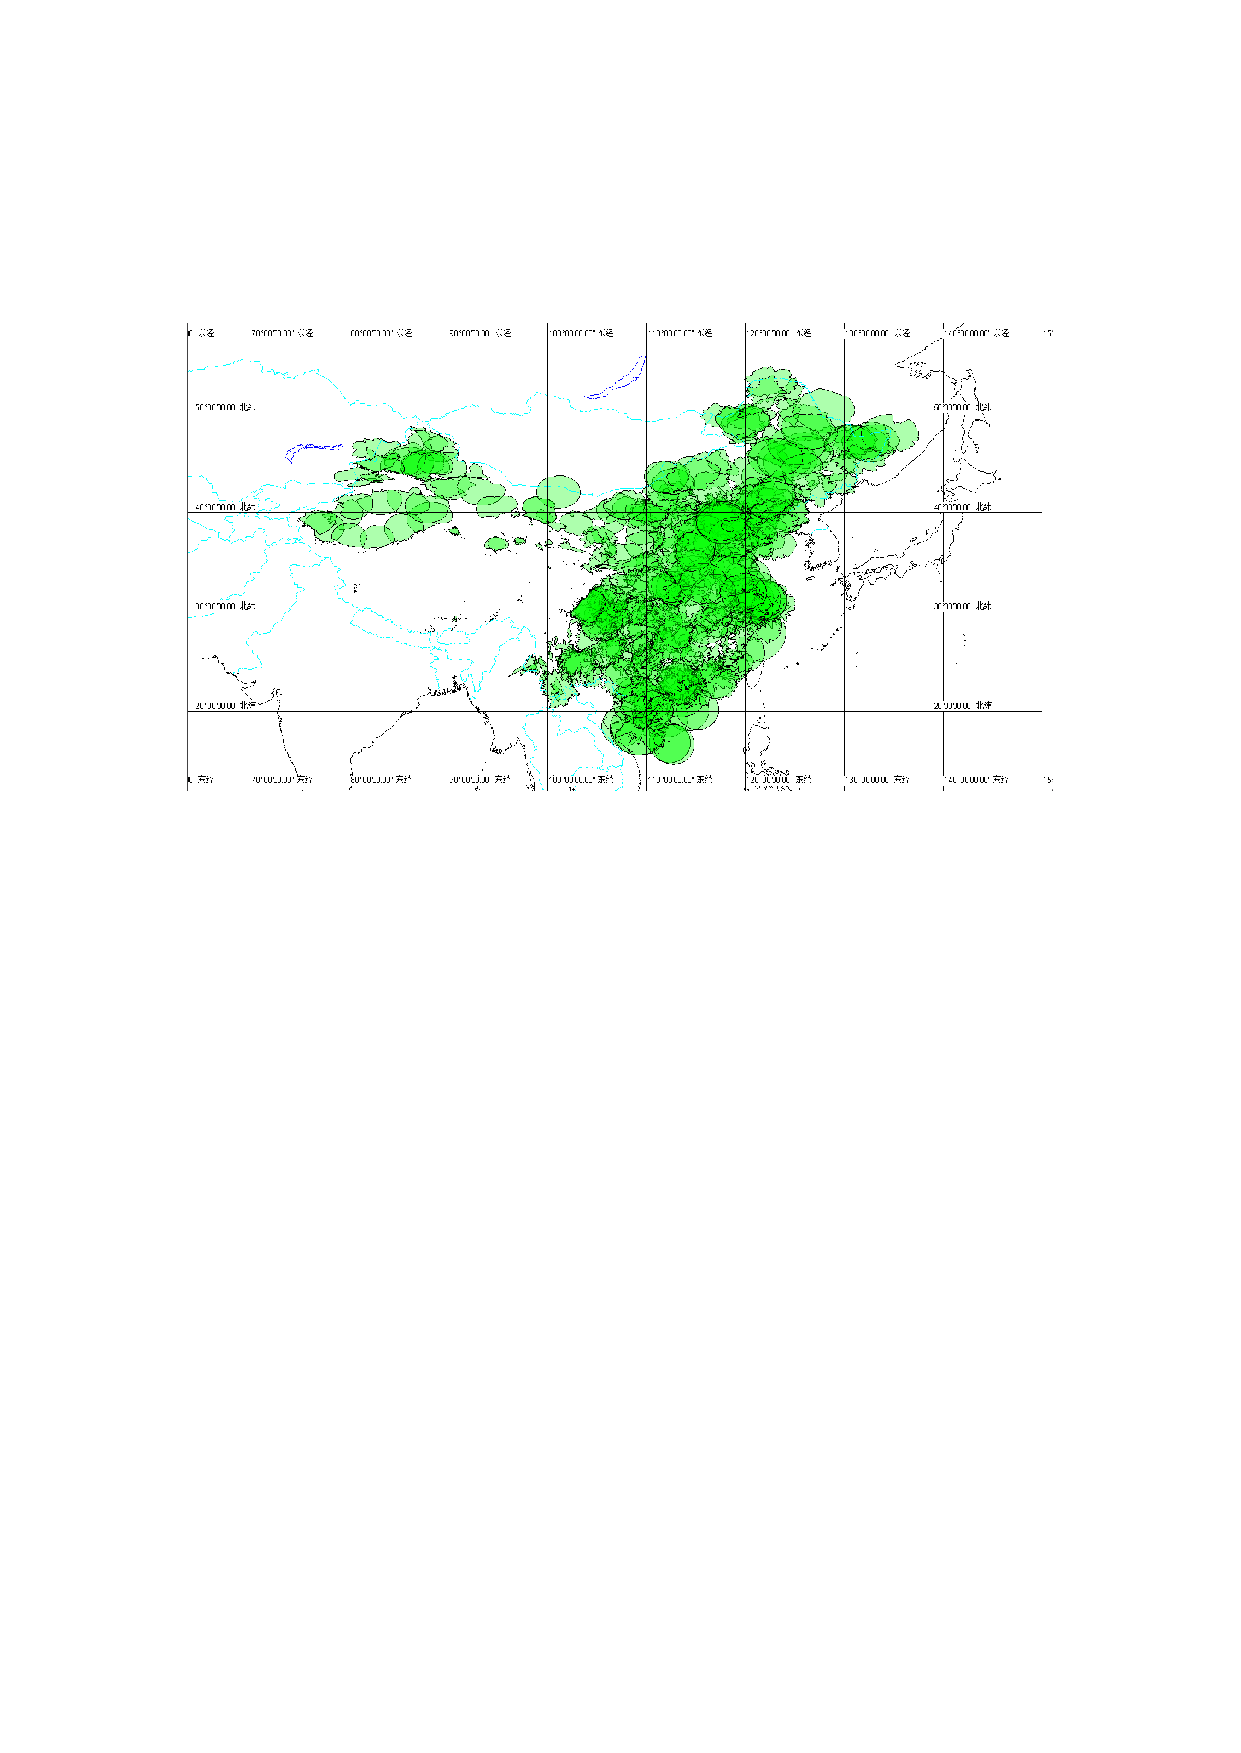
\includegraphics[width=13cm]{pic/china_3300m.pdf}
\caption{中国 3300m 空域 ADS-B 覆盖情况\protect\footnotemark}
\label{fig:china_3300m}
\end{figure}

\footnotetext{图片来源:参考文献\cite{e6}}

\begin{figure}[!htb]
\centering
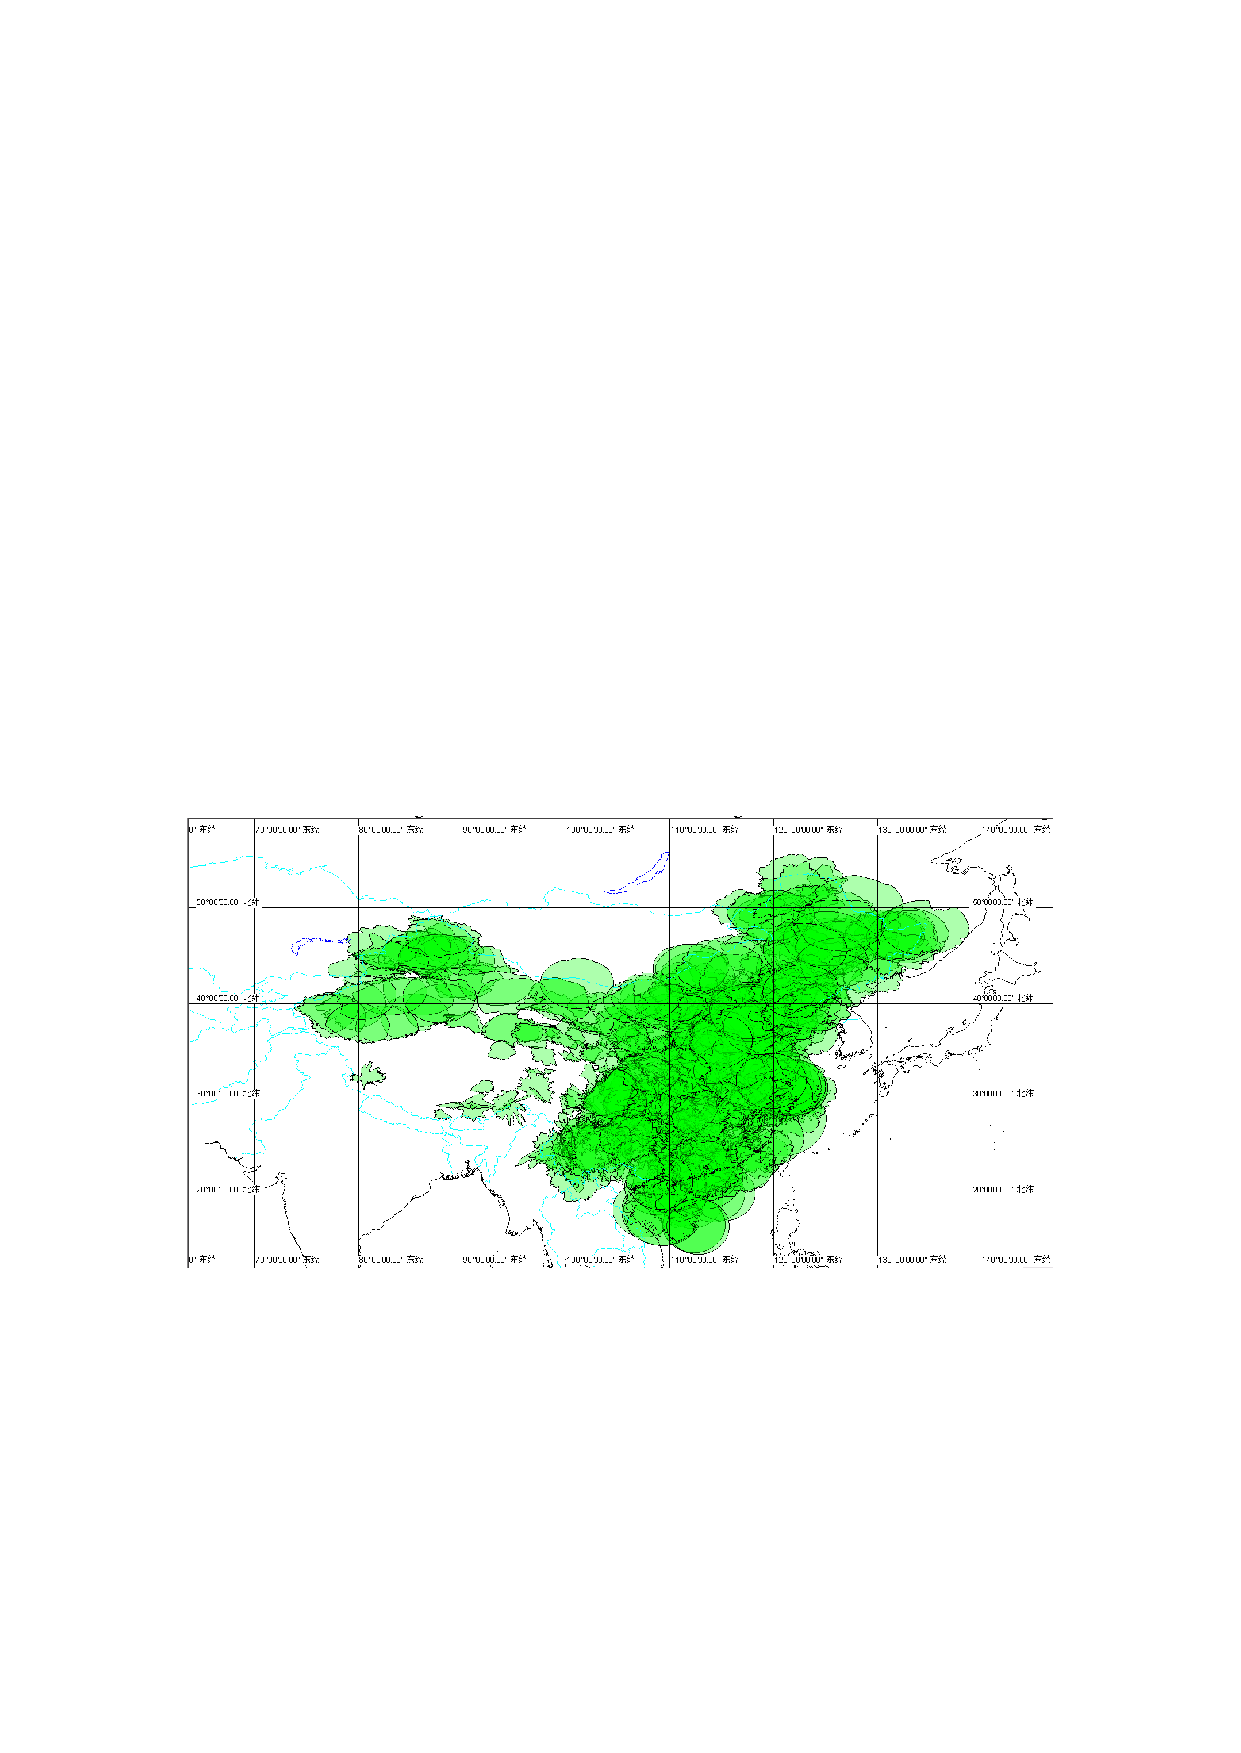
\includegraphics[width=13cm]{pic/china_6600m.pdf}
\caption{中国 6600m 空域 ADS-B 覆盖情况\protect\footnotemark}
\label{fig:china_6600m}
\end{figure}

\footnotetext{图片来源:参考文献\cite{e6}}

\begin{figure}[!htb]
\centering
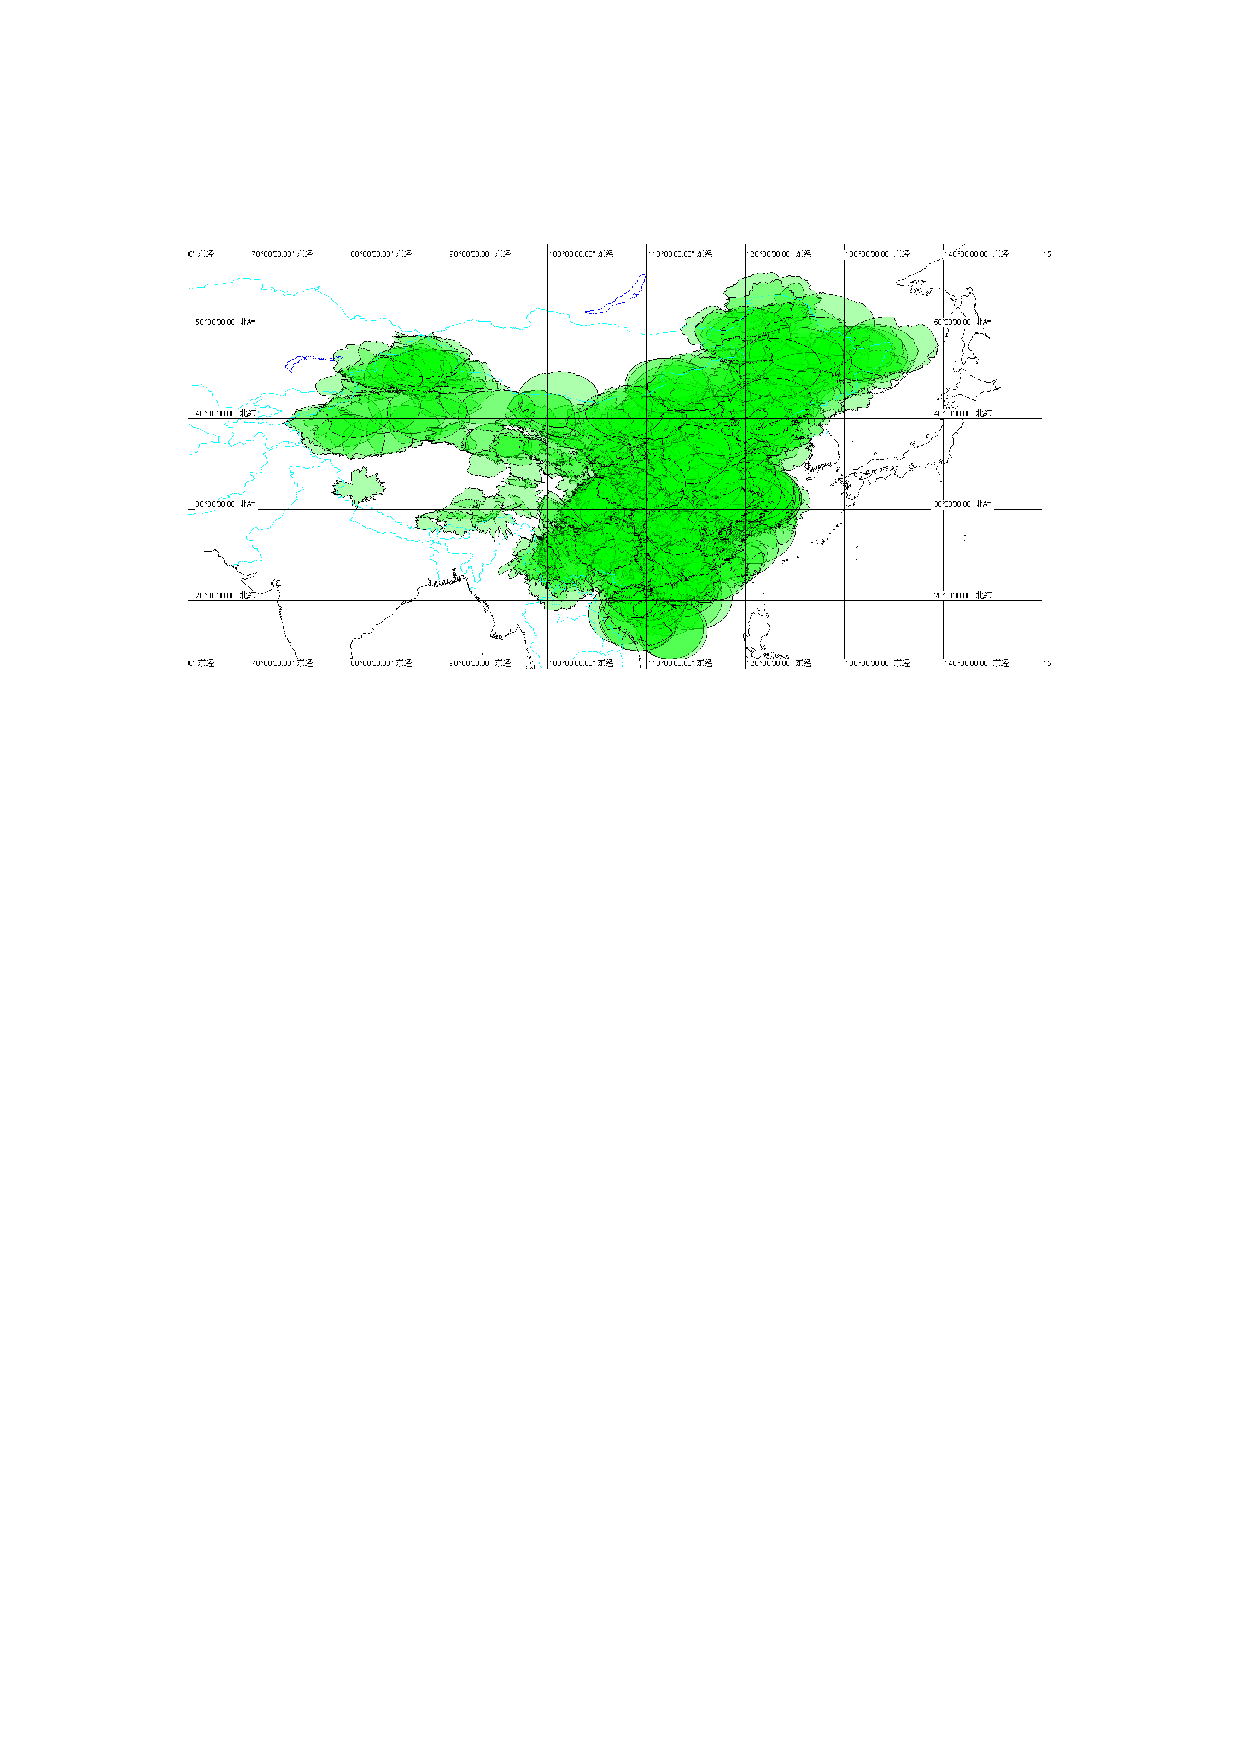
\includegraphics[width=13cm]{pic/china_8400m.pdf}
\caption{中国 8400m 空域 ADS-B 覆盖情况\protect\footnotemark}
\label{fig:china_8400m}
\end{figure}

\footnotetext{图片来源:参考文献\cite{e6}}

在中国南海,为满足 L642 路和 M771 路 ADS-B 监控控制需求,提升三亚 \acs{FIR} 的 ADS-B 监控能力,CAAC 在 FIR 内增设了 4 个 ADS-B 站。截至 2016 年 4 月 19 日文档发布期间,已有 4 个 ADS-B 站和 1 个 ADS-B 数据处理站完成了安装调试和现场验收测试,空中交通管制自动化系统已完成软件升级测试,即将投入运作,这一地区的监测范围将大大改善。

中方愿将 ADS-B 数据处理中心的 ADS-B 数据与周边国家/行政部门共享。

根据 ICAO 第十四次东南亚和孟加拉湾区域 ADS-B 实施工作组会议(SEA/BOB ADS-B WG/14)信息论文(IP,Information Paper)IP/3\upcite{e7}显示,自 2016 年起,中国一直在规划国家 ADS-B 项目,该项目由 308 个地面站和 3 级网络架构组成,用于处理和分发 ADS-B 数据。根据项目方案,所有的安装部署活动已经完成,所有的现场验收测试和飞行检查将于 2018 年底完成。ADS-B 服务的初步运营将于 2019 年初准备就绪。2019 年 7 月 1 日,ADS-B 在全国空域试运行。

\subsection{东南亚}

\subsubsection{印度尼西亚}

根据 ICAO 十四次 ADS-B 研究和实施研讨会(ADS-B SIFT/14)议信息论文(IP,Information Paper)IP/23 \upcite{e8}显示,澳大利亚、新加坡和印度尼西亚是全球实施 ADS-B 数据共享的领导者。到目前为止,印度尼西亚一直在执行国际民航组织关于与邻国(澳大利亚和新加坡)进行 ADS-B 数据共享的建议。

实施 ADS-B 监视的地区包括雅加达 FIR 和 Ujung Pandang FIR,飞行高度 FL290 至 FL460 的 A 级空域,以及前往印尼访问的使用 ADS-B 的外国注册飞机。如果飞机在印度尼西亚领空携带 ADS-B 发射设备,该设备必须符合经批准的 ADS-B 设备配置。

印度尼西亚 ADS-B 基站以及数据处理和共享中心的布置情况如图\ref{fig:Indonesia_integration}所示,印尼上空 ADS-B 覆盖范围的仿真模拟如图\ref{fig:Indonesia}所示。

\begin{figure}[!htb]
\centering
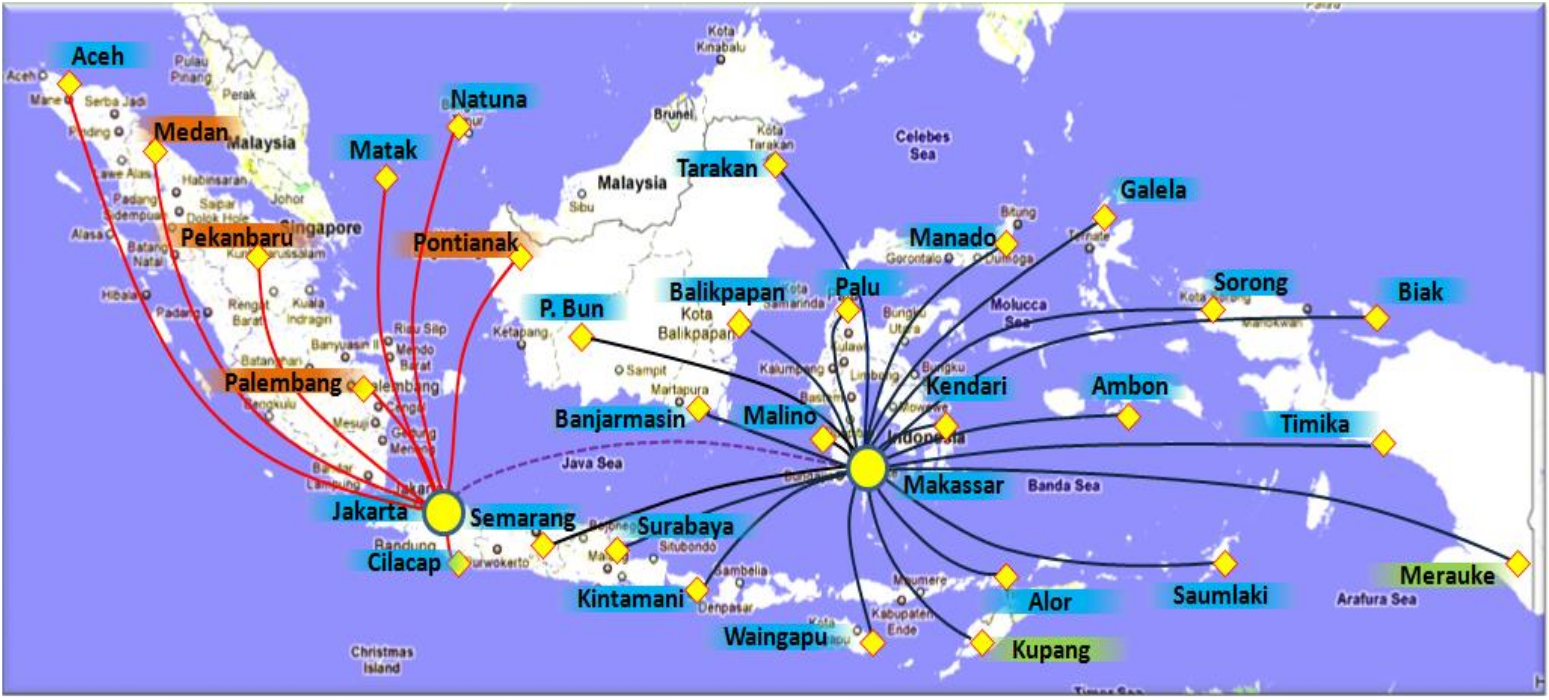
\includegraphics[width=14cm]{pic/Indonesia_integration.png}
\caption{印度尼西亚 ADS-B 基站布置情况\protect\footnotemark}
\label{fig:Indonesia_integration}
\end{figure}

\footnotetext{图片来源:参考文献\cite{e8}}

\begin{figure}[!htb]
\centering
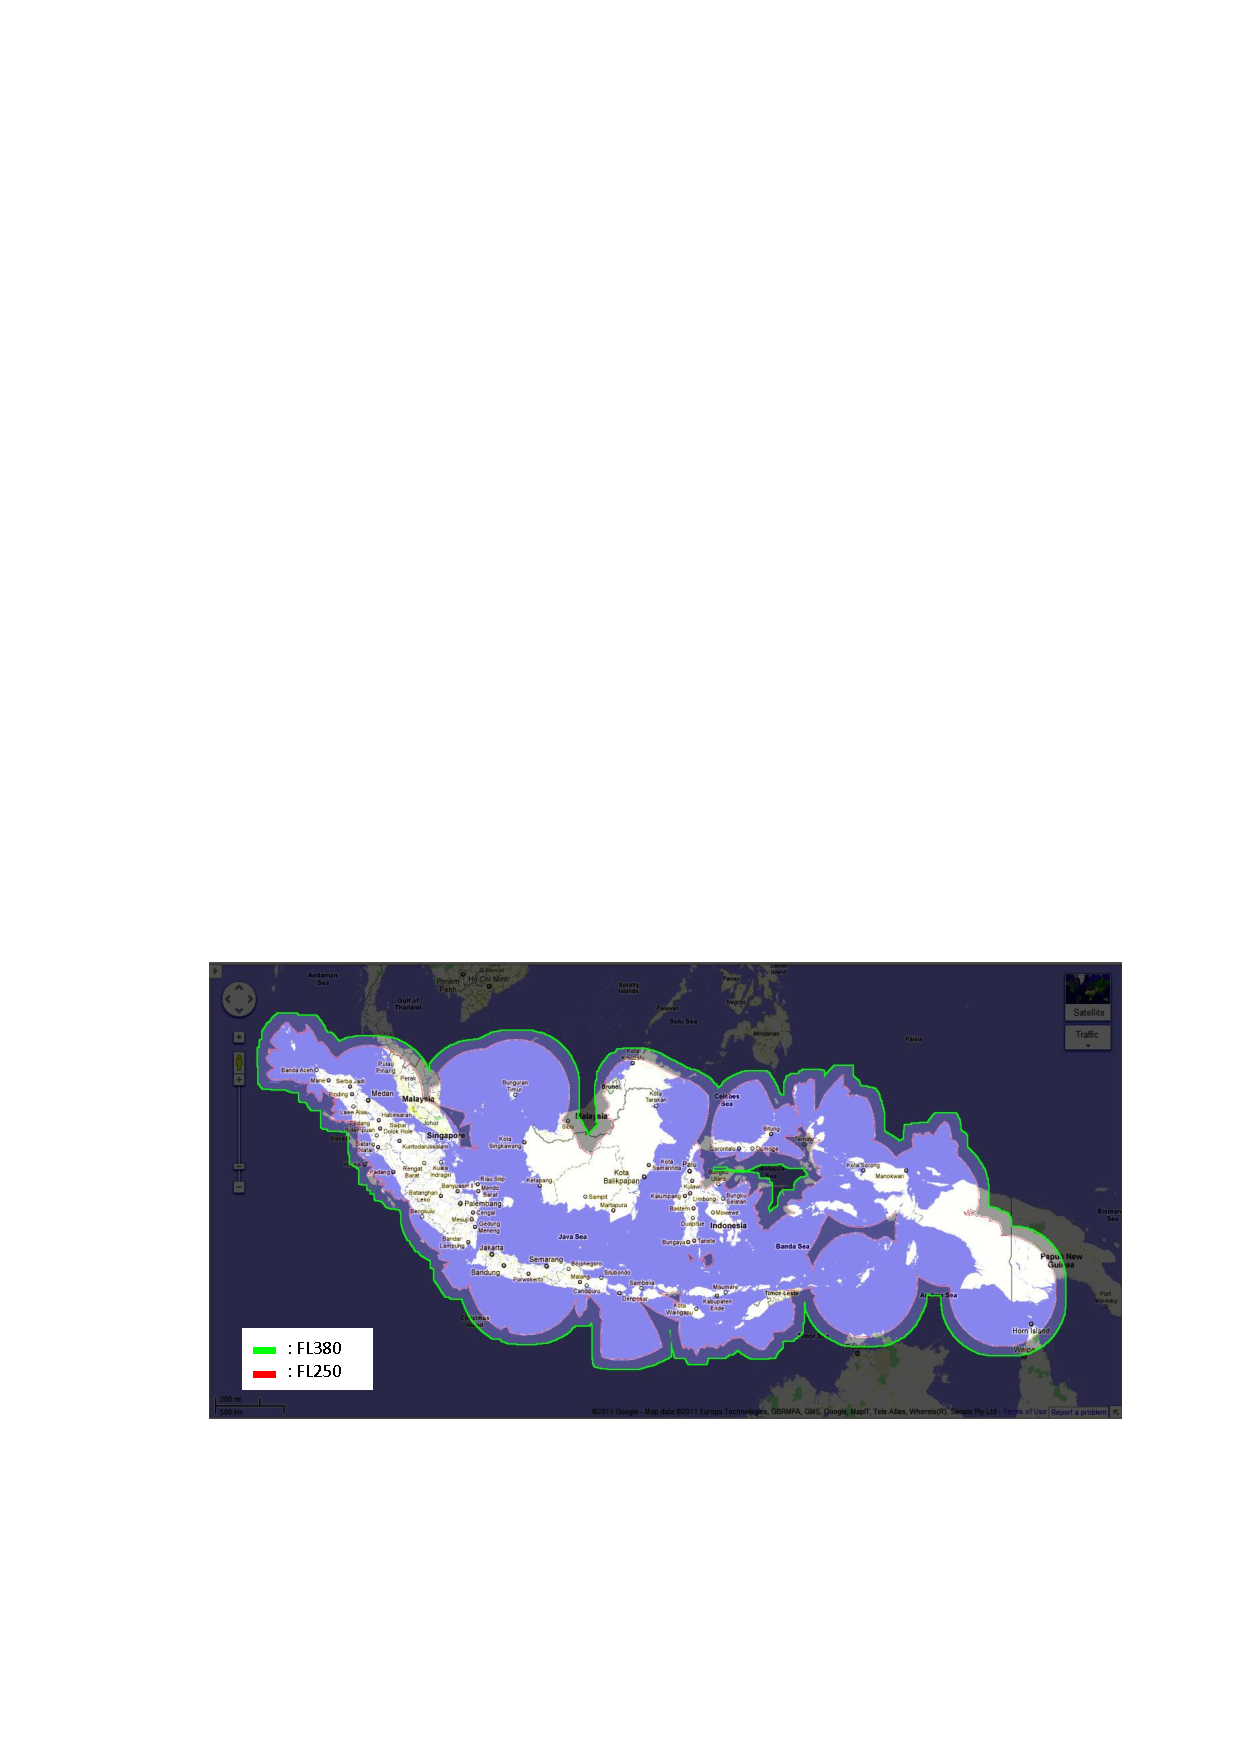
\includegraphics[width=14cm]{pic/Indonesia.pdf}
\caption{印度尼西亚 ADS-B 覆盖情况模拟\protect\footnotemark}
\label{fig:Indonesia}
\end{figure}

\footnotetext{图片来源:参考文献\cite{e8}}

\subsubsection{马来西亚}

根据 ICAO 第十三次东南亚和孟加拉湾区域 ADS-B 实施工作组会议(SEA/BOB ADS-B WG/13)信息论文(IP,Information Paper)IP/09\upcite{e9}显示,Genting ADS-B 站安装工作进展顺利,2016 年 12 月完成设置和用户验收测试。但是,Langkawi 的 ADS-B 安装工作由于安装规范的变更,完成时间较长。安装已于 2017 年 10 月完成,用户验收测试已于 2017 年 11 月初成功完成。

2017 年 11 月两个 ADS-B 基站监测数据记录显示,各方向覆盖范围均超过 250NM,如图\ref{fig:Malaysia}所示。两个监测站的 ADS-B 数据将被融合到多监视融合系统中进行进一步的观测和测试,然后才能进行验证投入使用。

\begin{figure}[!htb]
\centering
\begin{minipage}[t]{0.50\textwidth}
\centering
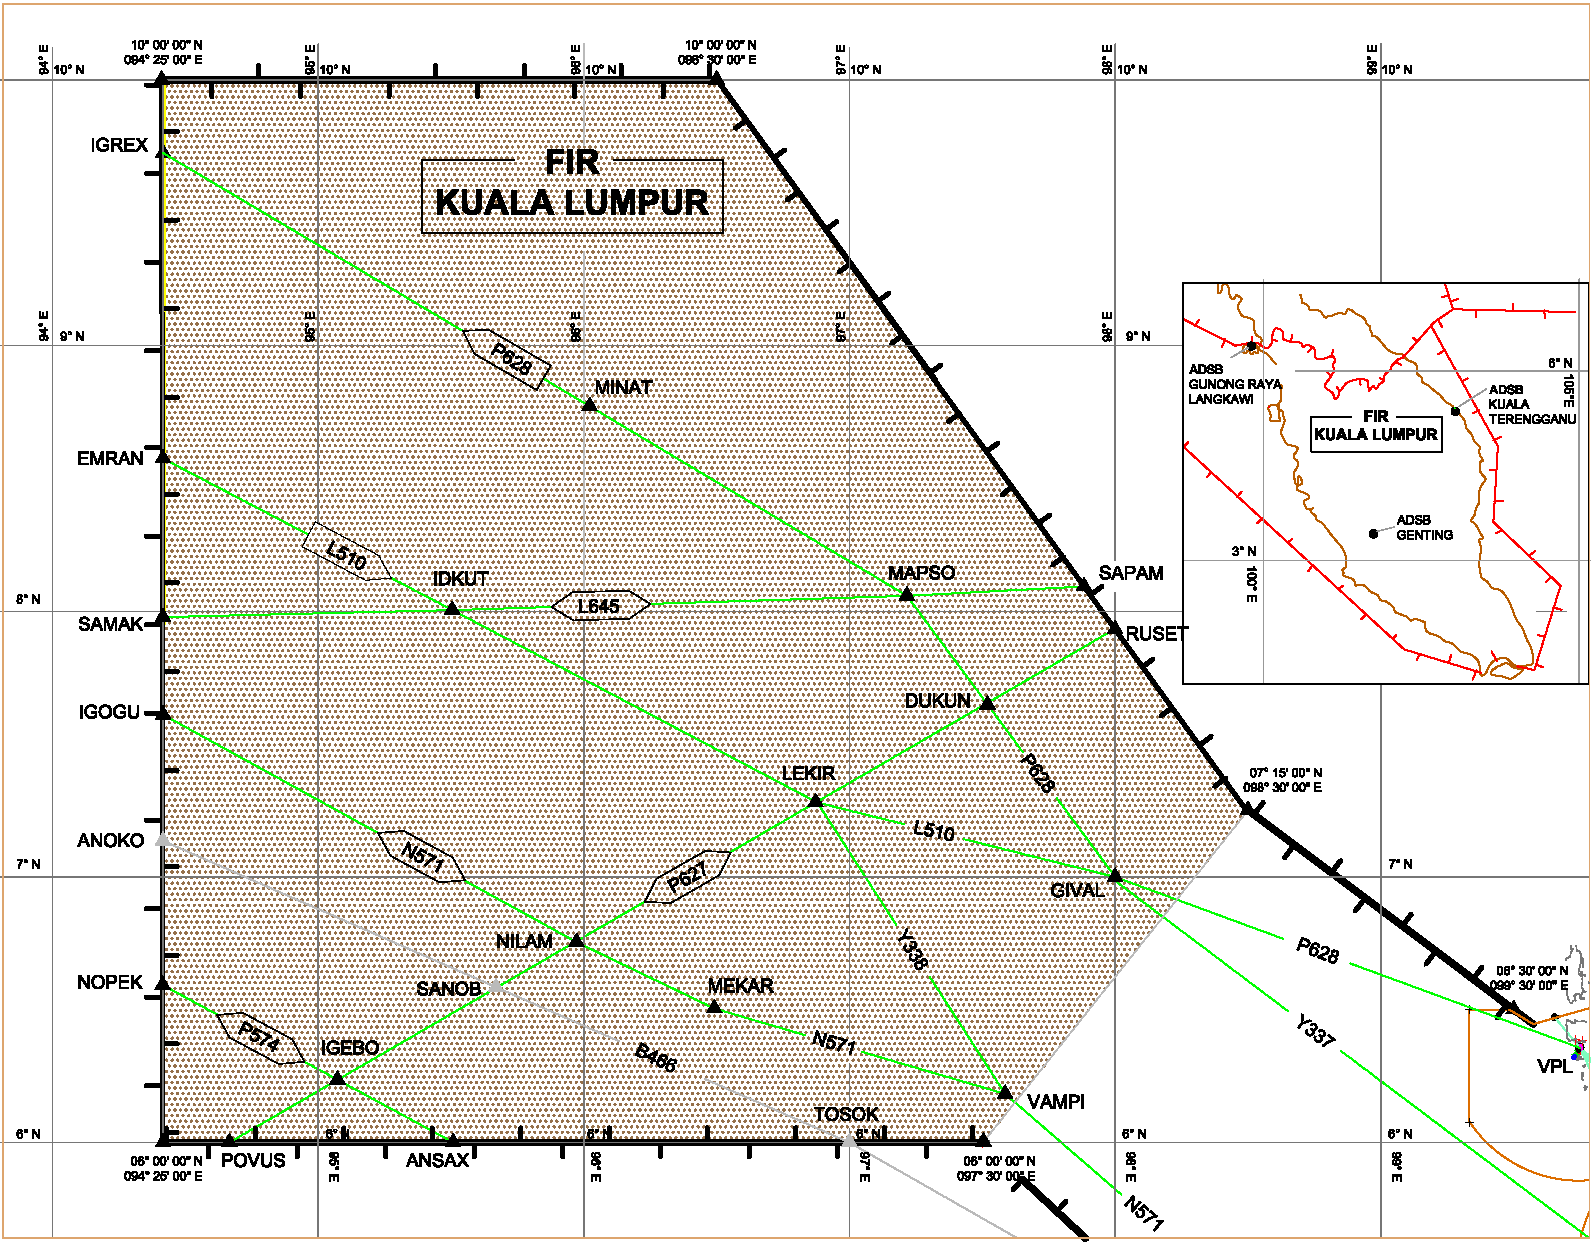
\includegraphics[width=8cm]{pic/malaysia_cover.png}
\caption{马来西亚 ADS-B 覆盖情况\protect\footnotemark}
\label{fig:malaysia_cover}
\footnotetext{图片来源:\url{http://aip.dca.gov.my/aip/eAIP/2017-09-07/html/eAIC/WM-eAIC-2017-03-en-MS.html}}
\end{minipage}
\begin{minipage}[t]{0.48\textwidth}
\centering
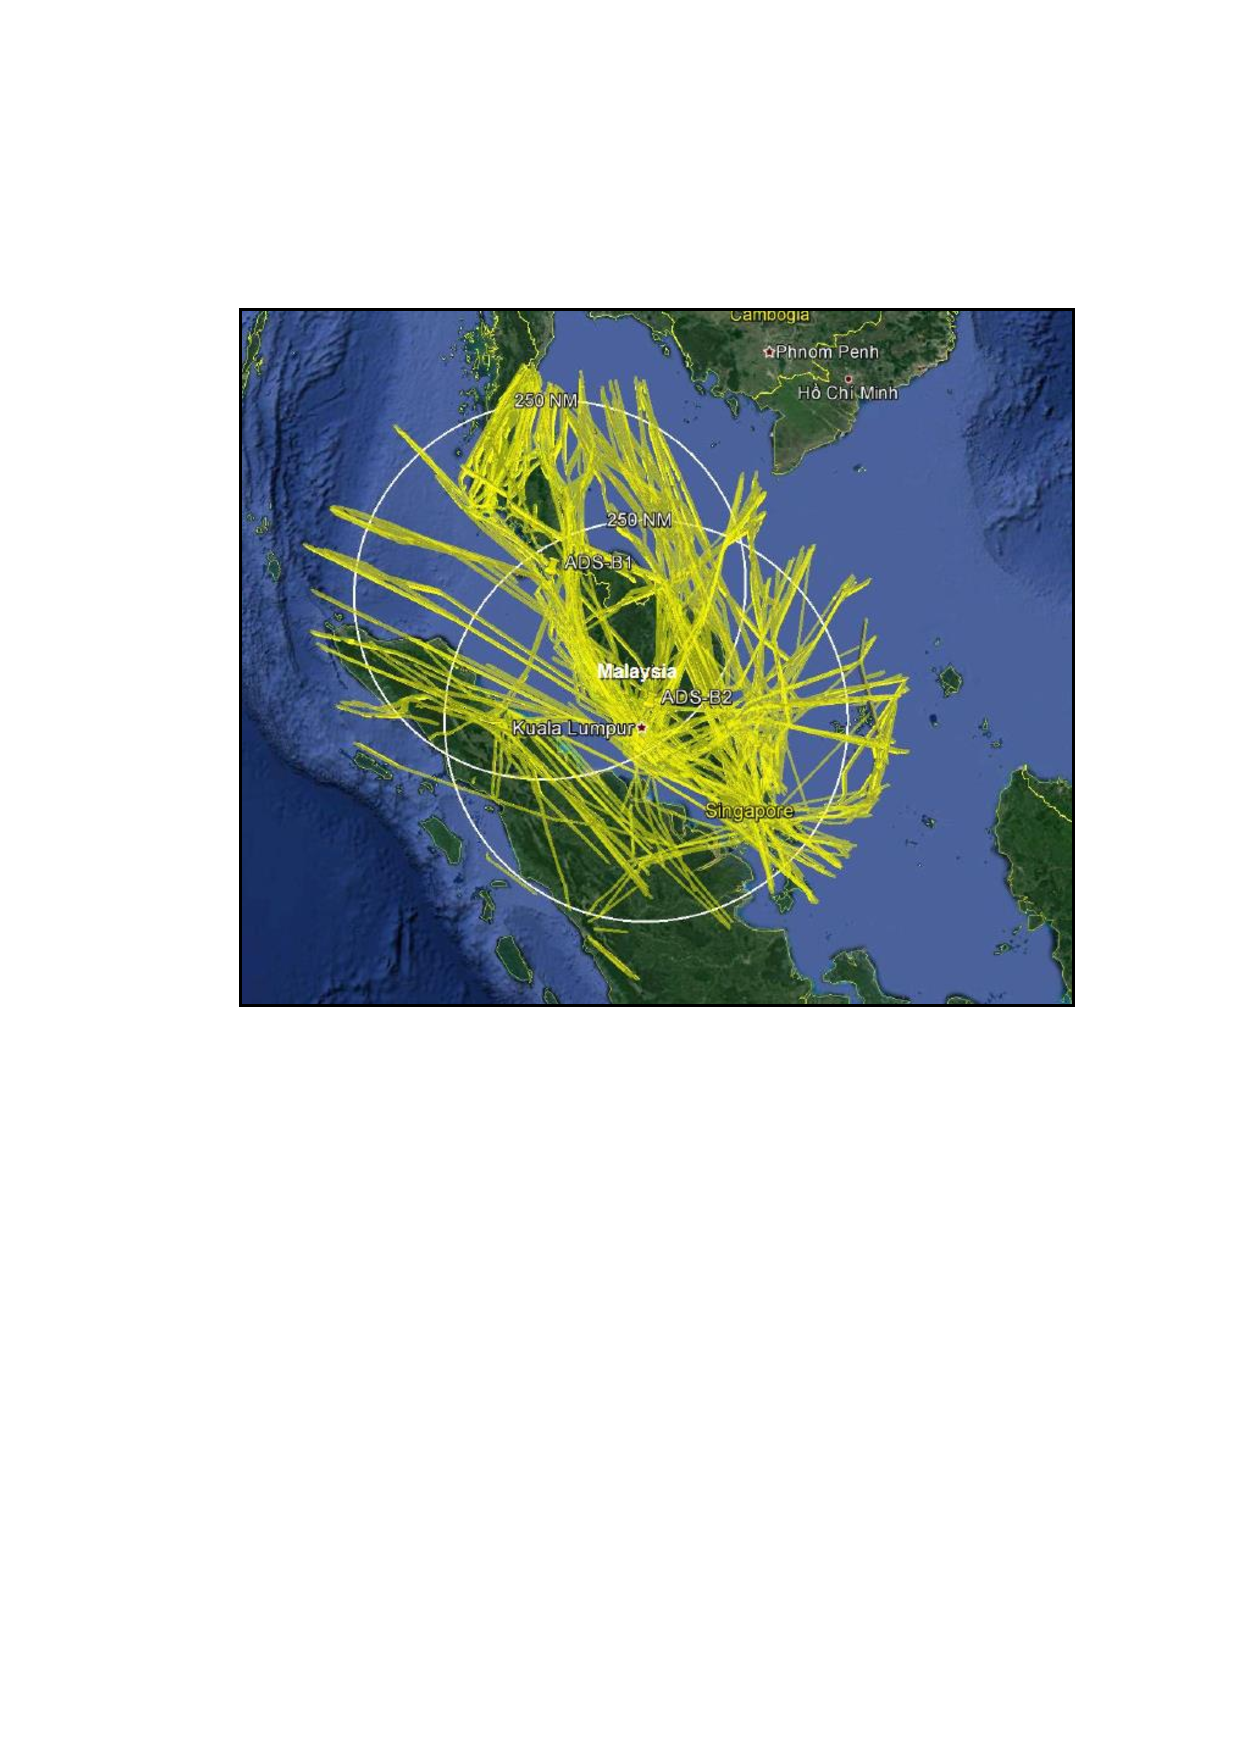
\includegraphics[width=7.5cm]{pic/Malaysia.pdf}
\caption{马来西亚 ADS-B 基站监测数据\protect\footnotemark}
\label{fig:Malaysia}\footnotetext{图片来源:参考文献\cite{e9}}
\end{minipage}
\end{figure}



\subsubsection{泰国}

根据 ICAO 第十二次东南亚和孟加拉湾区域 ADS-B 实施工作组会议(SEA/BOB ADS-B WG/12)信息论文(IP,Information Paper)IP/09\upcite{e10}显示,2006年,AEROTHAI 在其位于曼谷的总部安装了首个 ADS-B 地面站,可以 ASTERIX CAT 21 0.26 版本的格式输出信息,以供研发之用。2014 年,在清迈、Ubon Ratchathani、Udon Thani、Hat Yai、Samui 市等地增设了 5 个 ADS-B 地面站,并取得了良好的实验效果。这些地面站能够支持 ASTERIX CAT 21 1.4 版和 2.1 版格式。同样在 2014 年,在曼谷安装的第一个地面站升级为支持 ASTERIX CAT 21 1.4 版和 2.1 版格式。此外,所有 ADS-B 地面站均符合 ED-129 标准。

每个 ADS-B 地面站提供的覆盖范围在半径 250 海里和海拔 4.5 万英尺以内。目前泰国各地共设置了 6 个 ADS-B 地面站,20000 英尺及以上空域基本覆盖如图\ref{fig:thailand}所示,可为曼谷 FIR 20000 英尺及以上航路运行提供 ADS-B 监控服务。目前,上述 ADS-B 地面系统正在通过 \acs{CAAT} 的认证,预计于 2017 年完成(文献于 2016 年发布)。

\begin{figure}[!htb]
\centering
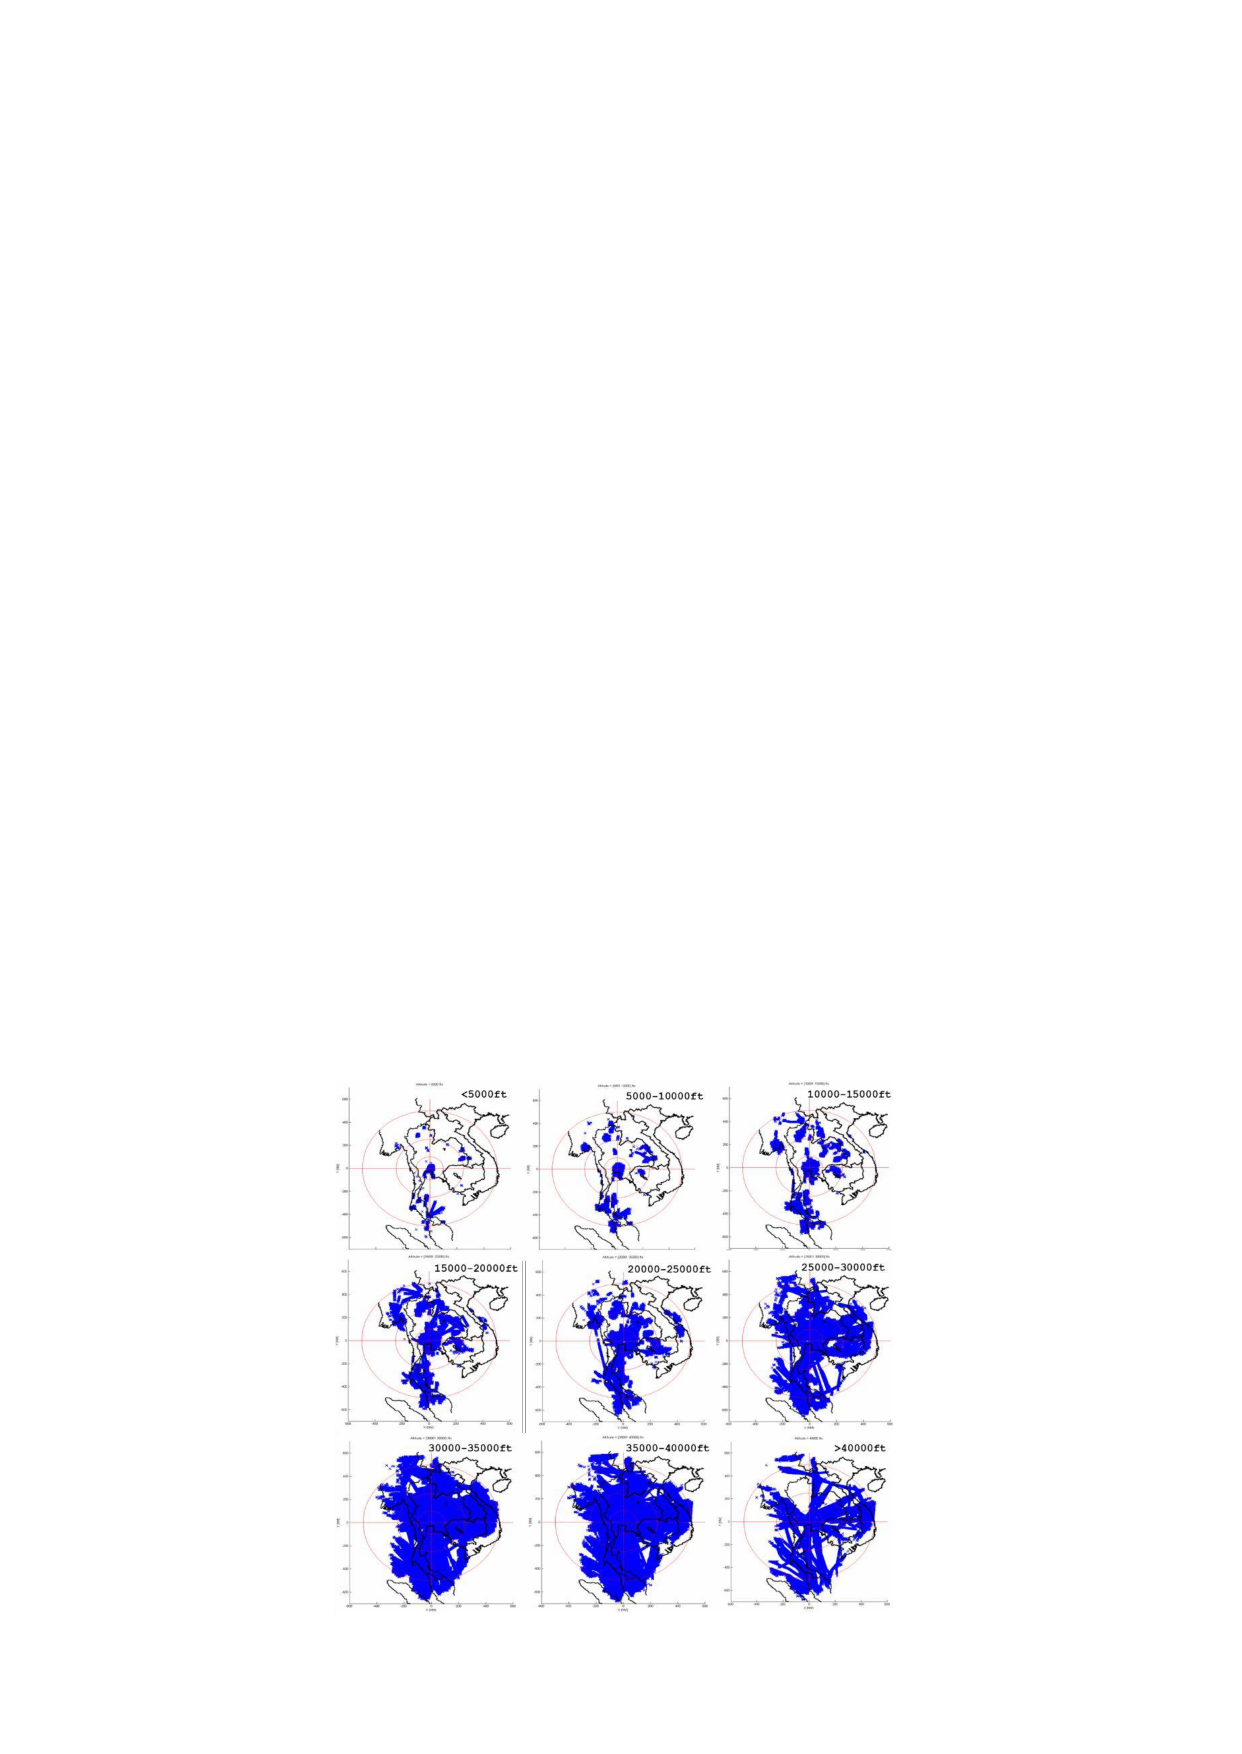
\includegraphics[width=14cm]{pic/thailand.pdf}
\caption{泰国 20000 英尺及以上空域 ADS-B 覆盖\protect\footnotemark}
\label{fig:thailand}
\end{figure}

\footnotetext{图片来源:参考文献\cite{e10}}

为了能够在较低的管制空域提供 ADS-B 服务,需要更多的 ADS-B 地面站。因此,这些地面站需要具备双重功能,即 ADS-B 和 WAM, 计划部署在泰国,旨在能够从 13000 英尺到 45000 英尺为航路运行提供 ADS-B 覆盖,从 2000 英尺到 11000 英尺为 8 个机场提供 TMA 运行服务。预计这些地面站的安装工作将于 2017 年中后期开始(文献于 2016 年发布)。

\subsubsection{菲律宾}

根据 ICAO 第十三次东南亚和孟加拉湾区域 ADS-B 实施工作组会议(SEA/BOB ADS-B WG/13)信息论文(IP,Information Paper)IP/17\upcite{e11}显示,在菲律宾的 \acs{CNS}/ATM 系统开发项目,截至 2017 年 10 月 16 日,已经完成 99.9\%, 包括安装新的监视系统,新监视系统包括 10 部雷达(5 部航路雷达和 5 终端区雷达),1 个 ADS-B 地面站和 3 台现有雷达系统的升级,这将覆盖菲律宾 80\% 的空域。海洋部分将被 ADS-C 覆盖。

菲律宾完成了位于马尼拉 ATM 中心的 1 个 ADS-B 地面站的安装。地面站符合 DO260B 标准。考虑到新的 CNS/ATM 系统仍处于过渡阶段,最初提出的 2017 年地面站(Kalayaan、Zambales 和 Pangasinan)将在 2018-2019 年底实施。另外 3 个场址(Jomalig 岛、General Santos 机场和 Ilocos Norte)计划在今后几年安装。有关 ADS-B 要求的相关规定已经在讨论中。

虽然在 CNS/ATM 项目下,ADS-C 覆盖范围将对菲律宾 100\% 的空域进行监视覆盖,但菲律宾也在考虑天基 ADS-B 技术,目前已经与供应商进行了初步讨论。

图\ref{fig:phillipine}显示了马尼拉 ATM 中心 ADS-B 的监控范围。

\begin{figure}[!htb]
\centering
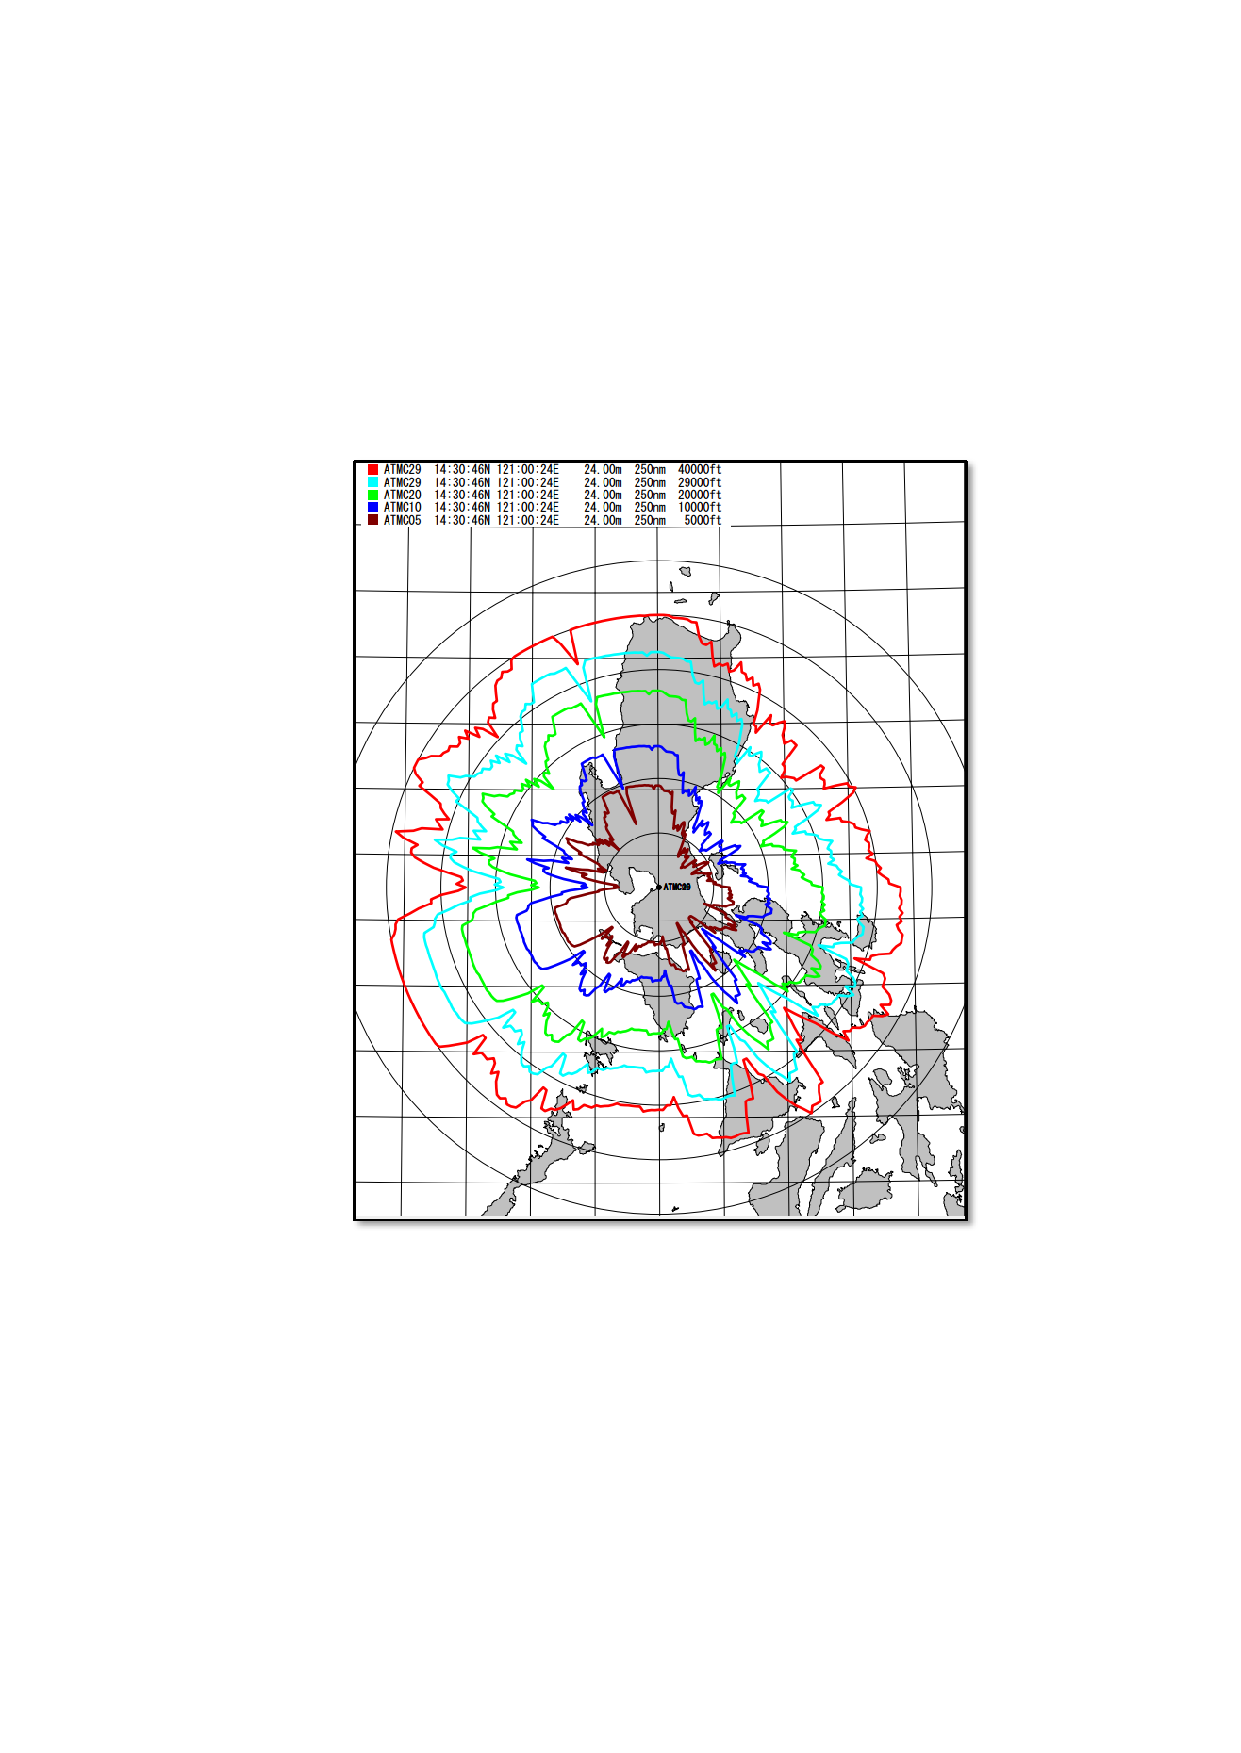
\includegraphics[width=9cm]{pic/phillipine.pdf}
\caption{菲律宾马尼拉 ATM 中心 ADS-B 监控范围\protect\footnotemark}
\label{fig:phillipine}
\end{figure}

\footnotetext{图片来源:参考文献\cite{e11}}

2015 年 10 月,菲律宾与新加坡签署 ADS-B 合作协议,在菲律宾巴塔拉扎为新加坡提供 ADS-B 数据和甚高频无线电设施。这部分覆盖了 ATS 航路 N884 和 M767 上的监视和 \acs{DCPC} 漏洞。




% !TEX root = ../document.tex

\chapter{星基 ADS-B 原理概述}

\section{传统陆基 ADS-B 系统的不足}

世界上大多数地区都是不受控制的空域。在没有雷达覆盖的地区,称为 NRA(非雷达空域),如海洋空域、极地地区或结构上落后的大陆地区,地面站的安装要么不可能,要么太昂贵。现在,这些地区的监视手段是程序管制,即飞行员在到达某个固定的航路点时报告位置,或者应用 ADS-C (Automatic Dependent Surveillance – Contract,合同式自动相关监视),通过一个点对点的数据链连接(FANS1/A/Satcom),由于带宽有限,它仅每 15 分钟发送一次位置和其他航班信息。在这两种情况下都不可能实现无缝和连续的飞行监视,并且需要一个相对较大的飞行间隔来保证安全。

陆基 ADS-B 地面站越来越多地部署,但是覆盖区域通常限制在几百公里。以澳大利亚航空服务为例,建造了大量的 ADS-B 地面站最终覆盖了飞行高度 FL300 以上的区域。

由于技术、运行和政治条件的限制,对基于陆基 ADS-B 的空中交通活动的全球监视似乎有些力有未逮,主要体现在\upcite{h2}:

\begin{itemize}
    \item 海洋全部覆盖要求在大量的浮标上部署 ADS-B 地面站
    \item 地面全部覆盖要求在不可接近区域部署和运营 ADS-B 地面站
    \item 全球空域分散,各个空域由大量当地 ATC 提供商运作
    \item 在不稳定地区的政治障碍阻碍了任何跨国监管和运作
\end{itemize}

传统陆基 ADS-B 系统主要由空中机载发射机和地面接收基站组成,受制于系统布置限制,一般沿民航航路航线、机场终端区等陆地区域进行布置,很难实现对洋区、沙漠、高山峡谷等特殊地区的覆盖。据统计,全球 90\% 的区域没有实现飞行监视覆盖。基于星基的 ADS-B 系统可有效克服陆基 ADS-B 系统的不足,可用于陆基 ADS-B /雷达难以覆盖或无法覆盖的空域,从而形成一个全球无缝的 ADS-B 覆盖网络\upcite{z1}。

\section{星基 ADS-B 的实验背景}
\label{sec:space_based_ads-b_experiment_back}

2008 年,德国航空航天中心(DeutschesZentrumfürLuft-und Raumfahrt,DLR)开始调查接收低地球轨道(LEO,Low Earth Orbit)卫星上的飞机广播 1090ES ADS-B 信号。这促成了 DLR 的星基 ADS-B 项目(AOS,ADS-B over Satellite),目标是开发一个用于 IOD(在轨演示)的 ADS-B 载荷,从而证明基于卫星的 ADS-B 监视在全球范围内的可行性。

该 AOS 在轨演示器能够接收、解码和转发所有 S 模式下行链路格式报文,这包括 DF17 扩展震荡 ADS-B 报文和 DF11 全呼应答。AOS 的在轨演示器是在 ESA 的 PROBA-Vegetation 卫星任务框架内进行的,并于 2013 年 5 月 7 日在法属圭亚那 Kourou 由欧洲最新的 VEGA 运载火箭成功发射。

DLR 的这个在轨演示器是演示和验证天基空中交通监视的第一步。一颗卫星搭载了具有太空生存能力的 ADS-B 接收机,由于预算、时间、特殊资源和 PROBA-Vegetation 卫星在功率和几何形状方面的限制,该 ADS-B 载荷采用了相对简单的天线和接收机设计。在未来提供无缝全球覆盖的运营系统将包括这样一组卫星,每个卫星都配备有精密的多通道 ADS-B 接收机和天线\upcite{h2}。

AOS 项目是星基 ADS-B 的第一次实验并且已经证明了星基 ADS-B 的可行性。该 IOD 的实验结果将为未来星基空中交通监视的目标铺平道路。

\section{星基 ADS-B 的工作原理}

基于星基的 ADS-B 系统借助低轨道通信卫星的强大覆盖能力,将 ADS-B 收发信机安装到通信卫星上。通信卫星通过其 ADS-B 设备接收飞机发送的 ADS-B 报告,再通过卫星通信信道下传给卫星地面站,卫星地面站通过地面网络将 ADS-B 报告传递给地面相关实体(如 ATC 中心、航空公司等),实现 ADS-B 全球覆盖,完成对飞机的全球飞行追踪和实时监控\upcite{e1}。星基 ADS-B 系统的结构布局原理如图\ref{fig:satellite_ads-b_arichitecture}所示。

星基(Satellite-Based) ADS-B 系统,同样称为“天基(Space-Based)”、“卫星增强(Satellite-Augmented)”或者“卫星重传(Satellite-Retransmitted)” ADS-B 系统\upcite{h1}。

\begin{figure}[htbp]
\centering
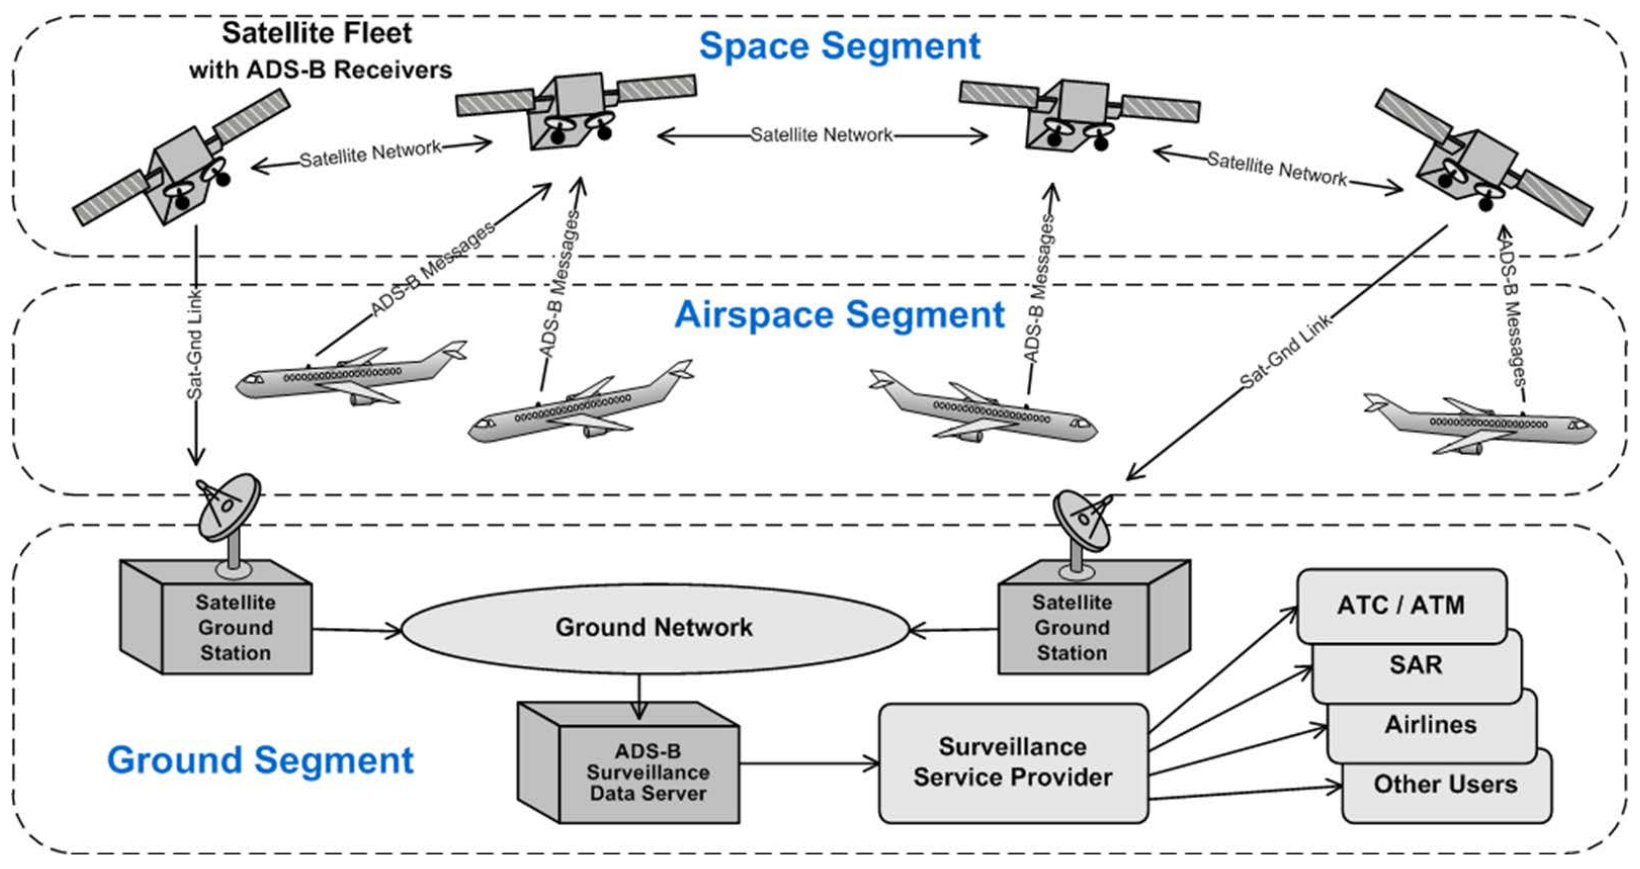
\includegraphics[width=15cm]{pic/satellite_ads-b_arichitecture.png}
\caption{星基 ADS-B 系统工作原理}
\label{fig:satellite_ads-b_arichitecture}
\end{figure}


% !TEX root = ../document.tex

\chapter{现阶段发展及应用情况}

\section{DLR 的 AOS 实验项目}

\subsection{项目概述}

根据\ref{sec:space_based_ads-b_experiment_back}节的内容,我们得知 DLR 的 AOS(ADS-B over Satellite)项目是世界上第一个天基 ADS-B 可行性验证实验项目。AOS 开发了一个 ADS-B 载荷,作为一个在轨演示器,搭载在 ESA(欧洲航天局)的 PROBA-Vegetation 卫星上,于 2013 年 5 月 7 日被发射到近地轨道上。AOS 是 DLR 空间系统研究所和 DLR 飞行指导研究所的合作项目,与卢森堡合作伙伴 SES TechCom Services 合作。

\renewcommand\arraystretch{1.5}
\begin{table}[htbp]
\centering
\caption{DLR 的 AOS 项目基本描述}
\label{tab:}
\begin{tabular}[b]{|p{2.5cm}<{\raggedleft}|p{12cm}<{\raggedright}|}
\hline
\textbf{目标} & 证明星基 ADS-B 监视的可行性 \par
            搭载于 ESA 的 Proba-V 卫星上的在轨演示器将验证一些关键参数,例如目标截获率、检测率和验证概率 \\
\hline
\textbf{项目持续时间} & 2011 年第一季度至 2014 年第二季度末 \\
\hline
\textbf{合作方} & Institute of Space Systems (RY) in Bremen, Germany \par
        Institute for Flight Guidance (FL) in Braunschweig, Germany \\
\hline
\textbf{贡献} & Institute RY: 开发和组装符合空间要求的 ADS-B 接收机和天线\par
Flight Calibration Services: 开发 ADS-B 接收机\par
Institute FL: ADS-B 数据的验证与评估 \\
\hline
\textbf{更多的合作} & RY with SES-ASTRA / ESA: 提供数据服务器 \\
\hline
\end{tabular}
\end{table}

\renewcommand\arraystretch{1.5}
\begin{table}[htbp]
\centering
\caption{ESA 的 Proba-V 小卫星任务描述}
\label{tab:esa_Proba-V_mission}
\begin{tabular}[b]{|p{2.5cm}<{\raggedleft}|p{12cm}<{\raggedright}|}
\hline
\textbf{主承包商} & QinetiQ Space nv \\
\hline
\textbf{卫星质量} & 约 140kg\\
\hline
\textbf{运载火箭 }& Vega 火箭\\
\hline
\textbf{发射日期} & 2013 年 5 月 7 日 \\
\hline
\textbf{发射场} & 法属圭亚那航天中心(库鲁)\\
\hline
\textbf{发射提供商} & Arianespace \\
\hline
\textbf{轨道} & 太阳同步轨道,海拔 820 公里,倾角 98.73$^\circ$,飘移限制在 10:30AM 到 11:30AM  \\
\hline
\textbf{通信} & 卫星的控制与通信通过比利时 Redu 地面站 \\
\hline
\textbf{主要任务} & 植被扫描仪 \\
\hline
\textbf{载荷} & ADS-B、高能粒子传感器、氮化镓 X 波段功率放大器 \\
\hline
\end{tabular}
\end{table}

ESA Proba-V 卫星自 2013 年 5 月 7 日起进入地球轨道, 其有效载荷包括一个专用接收器,用于接收飞机 ADS-B 信号。5 月 23 日,该实验首次开启,在两小时内在 820 公里的高度记录了 12000 条 ADS-B 信息。飞越苏格兰的 A320 飞机是 DLR 新型接收机从太空“看到”的第一架飞机,证明可以从太空跟踪飞机。


\subsection{体系结构}

Proba-V 上的 ADS-B 接收器由卢森堡的 DLR 和 SES TechCom 提供,主要目的是在飞行代表性配置中测试(空间限定)ADS-B 电路板以评估 TID(总电离剂量)。

ADS-B 接收器(1090ES RX)的基本设计概念是单转换超外差接收机,由 1090MHz 下变频调至中频 70MHz,70MHz 下的 IF 采样由一个 105Msps(每秒兆采样次数)的 16 位 ADC 完成。该 ADS-B 单转换超外差接收机概念如图\ref{fig:dlr_ads-b_receiver}所示\upcite{e2}。

\begin{figure}[htbp]
\centering
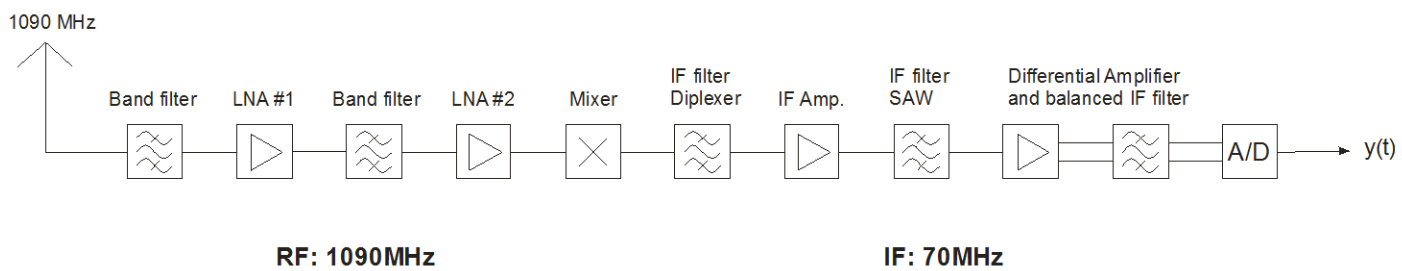
\includegraphics[width=15cm]{pic/dlr_ads-b_receiver.png}
\caption{单转换超外差接收机}
\label{fig:dlr_ads-b_receiver}
\end{figure}

\begin{figure}[htbp]
\centering
\subfigure[载荷原型]{
\begin{minipage}[b]{0.3\linewidth}
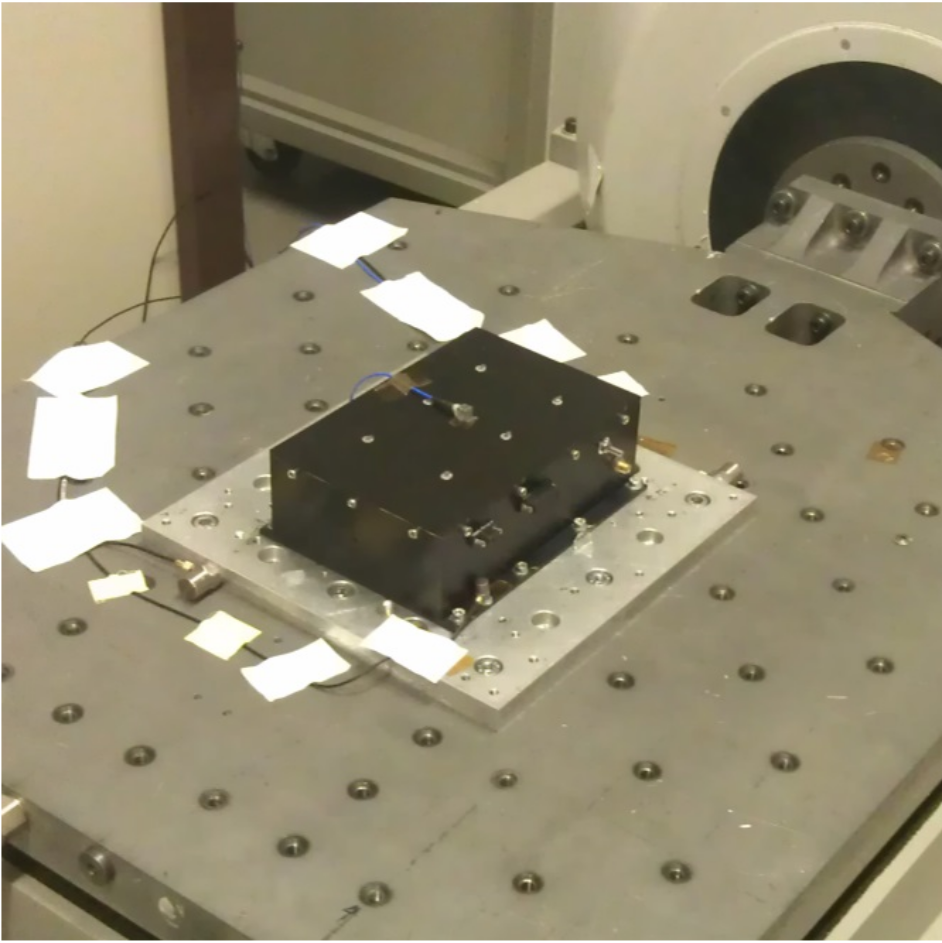
\includegraphics[width=1\linewidth]{pic/aos_ads-b_payload_2.png}
\end{minipage}}
\subfigure[安装位置]{
\begin{minipage}[b]{0.3\linewidth}
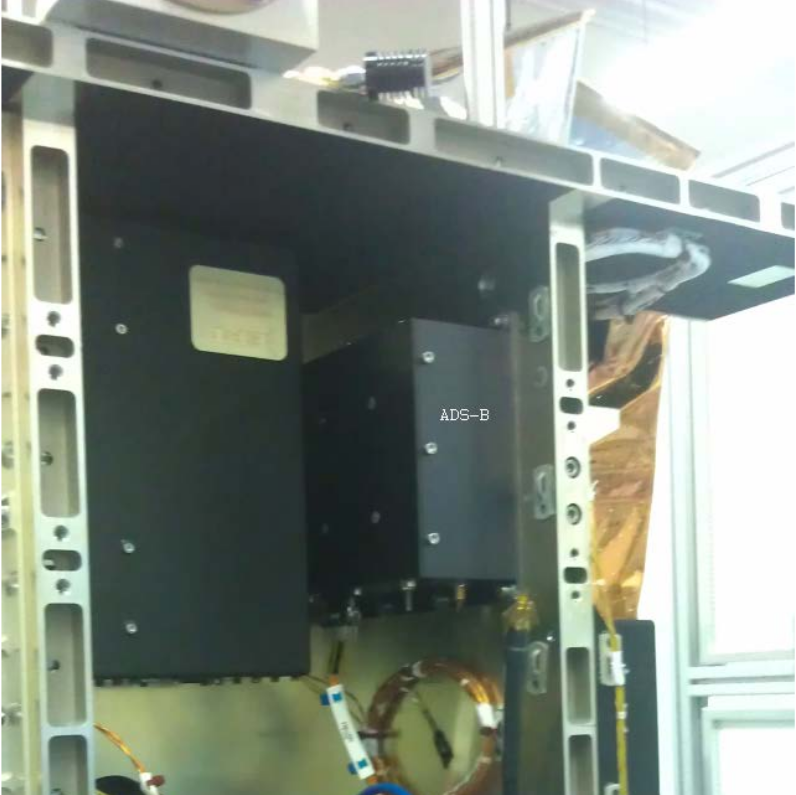
\includegraphics[width=1\linewidth]{pic/aos_ads-b_payload_1.png}
\end{minipage}}
\subfigure[卫星原型]{
\begin{minipage}[b]{0.3\linewidth}
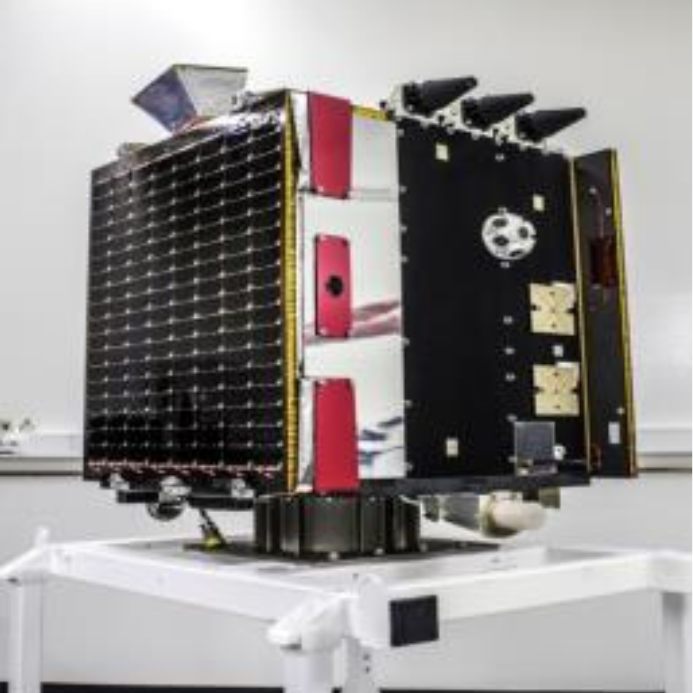
\includegraphics[width=1\linewidth]{pic/aos_ads-b_payload_3.png}
\end{minipage}}
\caption{Proba-V 卫星上搭载的 ADS-B 载荷}
\label{fig:aos_ads-b_payload}
\end{figure}

\begin{figure}[htbp]
\centering
\begin{minipage}[t]{0.48\textwidth}
\centering
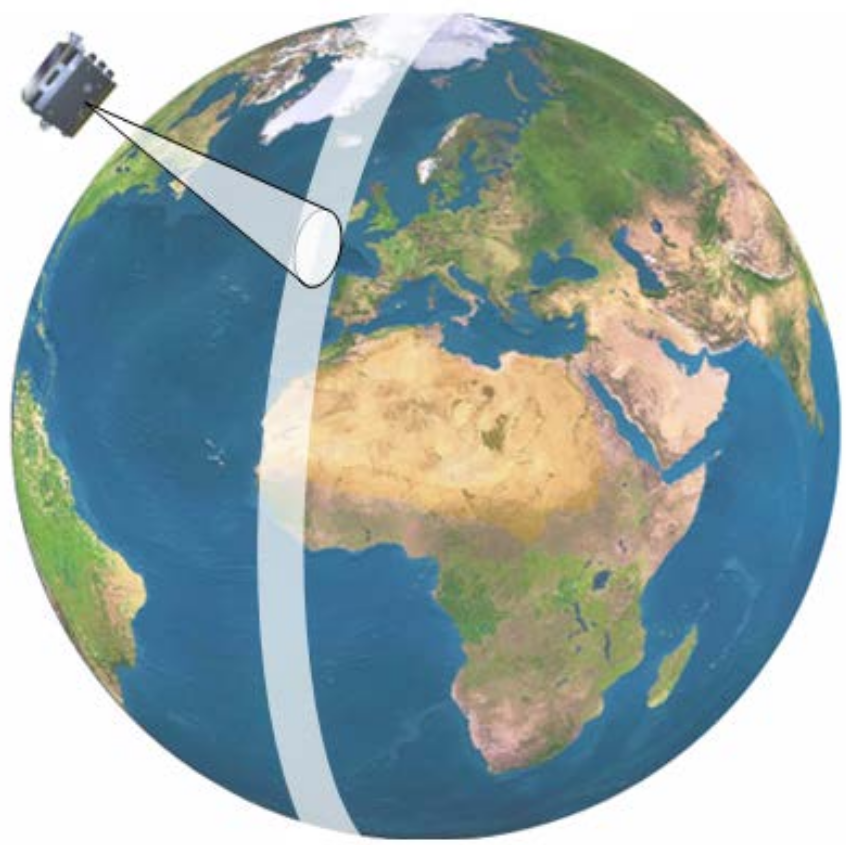
\includegraphics[width=6cm]{pic/aos_in_orbit.png}
\caption{技术验证阶段的单颗卫星}
\label{fig:aos_in_orbit}
\end{minipage}
\begin{minipage}[t]{0.48\textwidth}
\centering
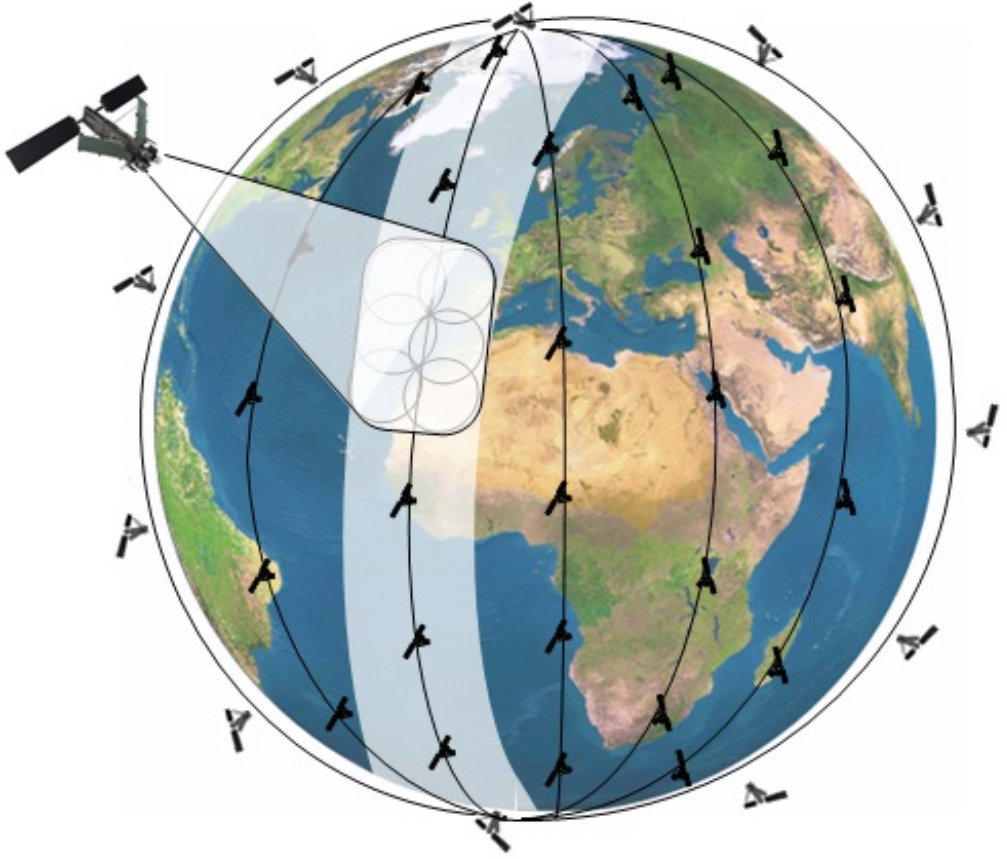
\includegraphics[width=7.2cm]{pic/aos_in_future.png}
\caption{未来全球卫星组网方案}
\label{fig:aos_in_future}
\end{minipage}
\end{figure}

\subsection{实验结果}

图\ref{fig:ADS-B_Auto6}展示了 2014 年 2 月 11 日在世界范围内记录的飞机航迹,每个红点代表卫星在其轨道上通过飞机时所看到的飞机航迹段。Proba-V 卫星的天线覆盖范围为纵向约 1200 公里,横向延伸至卫星飞行方向 500 公里,可逐条扫描全球空域。

\begin{figure}[htbp]
\centering
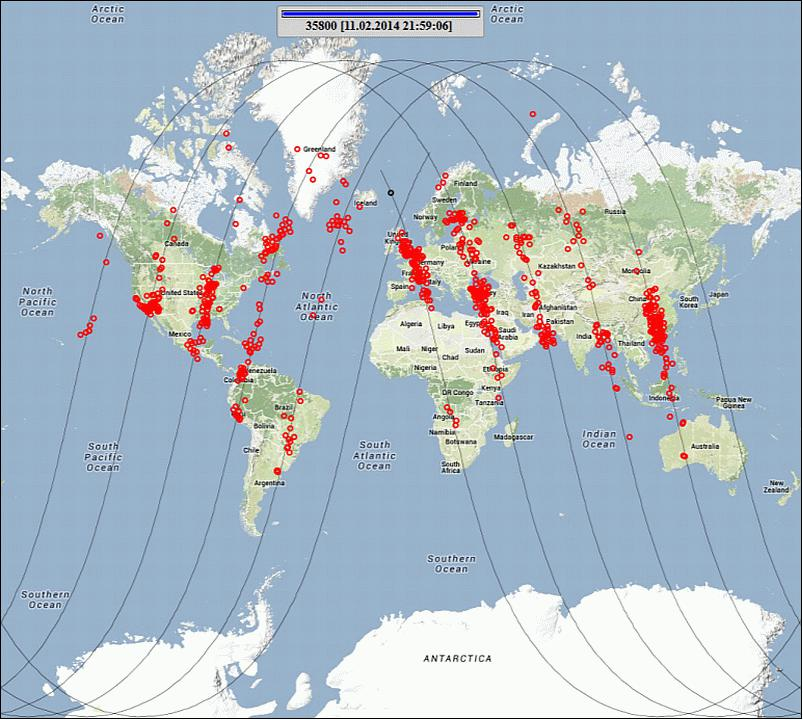
\includegraphics[width=10cm]{pic/ADS-B_Auto6.jpeg}
\caption{AOS 在世界范围内记录的飞机航迹(2014 年 2 月 11 日)}
\label{fig:ADS-B_Auto6}
\end{figure}

在空间接收 ADS-B 报文的最重要方面是卫星上 1090 MHz 扩展电文信号的接收条件。与基于地面的 ADS-B 监视相比,陆基 ADS-B 最大接收范围可达 300 公里,而在 820 公里高度轨道运行的 LEO 卫星与飞机之间的信号路径要长得多,这导致 ADS-B 的信号电平较低。接收器必须通过相关处理几乎在噪声水平上检测 S 模式信号。

实验得到了卫星天线覆盖区中不同区域接收到的 ADS-B 报文数量分布的直方图,如图\ref{fig:ADS-B_Auto5}所示,该图显示了 2014 年 5 月收到的所有位置消息的直方图。值得注意的是两个峰值,一个在卫星运动方向前方,峰值较低,另一个在卫星运动方向后方,峰值较高。这个谱的分布是不对称的,这由许多原因引起,比如卫星上的贴片天线的安装位置不对称、安装在卫星下侧的其他设备和在下表面的前边缘上突出的太阳能电池板。

\begin{figure}[htbp]
\centering
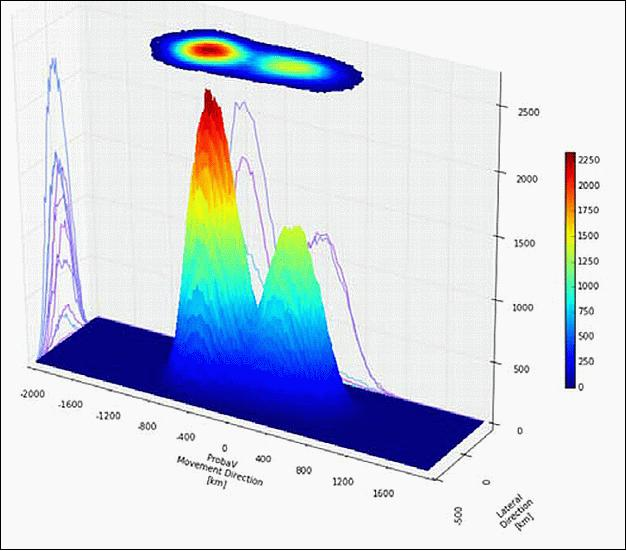
\includegraphics[width=10cm]{pic/ADS-B_Auto5.jpeg}
\caption{所有接收到的位置信息在天线覆盖区中的分布直方图}
\label{fig:ADS-B_Auto5}
\end{figure}

直方图的峰值可以通过卫星的接收天线和飞机的发射天线的天线辐射图来解释。图\ref{fig:ADS-B_Auto4}显示了安装在 Proba-V 卫星最低点面板上的 ADS-B 贴片天线的实测辐射图。合成的天线辐射图在卫星移动方向整体呈椭圆形状,最大灵敏度略低于卫星下方的最低点方向。

飞机装有两个 ATC 天线,一个在机身顶部,一个在机身底部,它们交替发射。由于几何因素限制,卫星将接收来自顶部天线的信号。顶部天线典型的垂直天线辐射模式如图\ref{fig:antenna_of_plane}所示。

\begin{figure}[htbp]
\centering
\begin{minipage}[t]{0.48\textwidth}
\centering
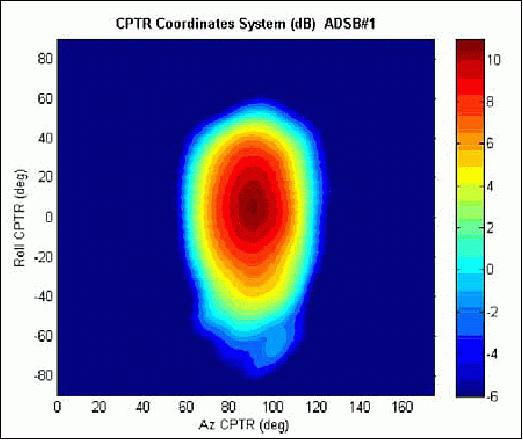
\includegraphics[width=7.5cm]{pic/ADS-B_Auto4.jpeg}
\caption{Proba-V 卫星天线辐射图}
\label{fig:ADS-B_Auto4}
\end{minipage}
\begin{minipage}[t]{0.48\textwidth}
\centering
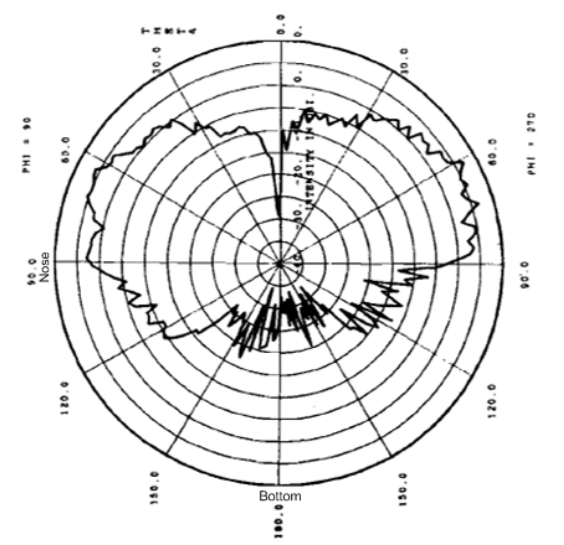
\includegraphics[width=6.5cm]{pic/antenna_of_plane.png}
\caption{顶部安装的 L 波段天线的垂直天线辐射图}
\label{fig:antenna_of_plane}
\end{minipage}
\end{figure}

\subsection{项目意义}

这次星载 ADS-B 接收验证实验的创举,将带来更多的在轨验证任务。ESA 与 Thales 德国签订合同,开发下一代 ADS-B 系统,该系统正在按计划进行,同时带来了卢森堡航天界(如 LuxSpace)的大力参与,将 TRITON 微小卫星平台作为以后的实验平台\upcite{h2}。

Proba-V 卫星实验项目取得了多个成果,主要包括:

\begin{itemize}
    \item 接收器的 FPGA 固件中包含一项特殊功能:允许上载新配置文件并通过远程访问激活这些配置。到目前为止,在任务运行期间,已成功测试了几次;

    \item 开发了改进的 S 模式相关机制,这得益于脉冲序列从第一个到第五个前导脉冲的相位相干性。在实验室测试中,可以显示报文检测率显著增加;

    \item 通过为 DF17 中的 112 个 S 模式数据位生成并保存“低置信度位”,增加了一次可以提高后处理报文解调成功率的机会;

    \item 卫星上的 ADS-B 接收器是同类中的第一个实验,接收从飞机发射的 1090ES ADS-B 电文信号。因此无法根据以往经验或任何结果进行系统设计。
\end{itemize}

Proba-V 卫星在实验中也遇到了一些困难,主要包括:

\begin{itemize}
    \item 由于卫星在大约 820 公里的高度,而飞机在 0 到 12 公里的高度,距离会导致接收的信号幅度过低从而导致信号丢失;

    \item 由于卫星天线垂直辐射图和飞机天线垂直辐射图的形状不同,会导致信号损失;

    \item 当到达卫星 ADS-B 天线的消息在时间上重叠(交织)时,ADS-B 接收机无法对其进行解码;

    \item 卫星的速度约为 27000 公里/小时,这导致每个检测到的飞机的观察时间有限,最多约 3 分钟。
\end{itemize}

这些困难提供了巨大的借鉴意义,为星基 ADS-B 技术发展中探明了一些需要克服的难点问题。

\section{Aireon 星基 ADS-B 系统}

\subsection{系统概述}



\begin{figure}[htbp]
\centering
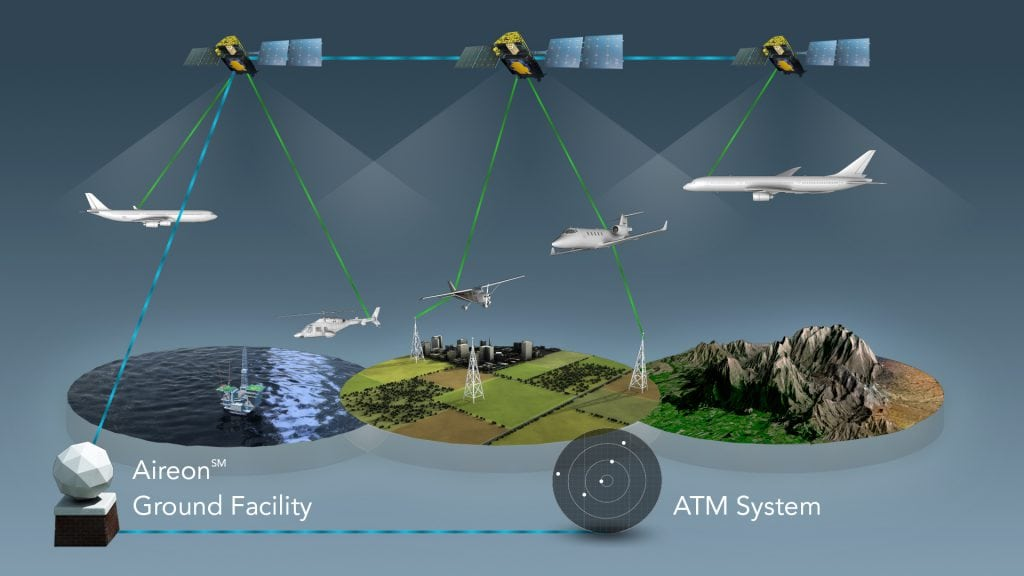
\includegraphics[width=15cm]{pic/Aireon_GlobalSpaceBasedADSB_Coverage_Diagram-1024x576.jpg}
\caption{Aireon 天基 ADS-B 系统布局原理}
\label{fig:Aireon_GlobalSpaceBasedADSB_Coverage_Diagram}
\end{figure}

\begin{figure}[htbp]
\centering
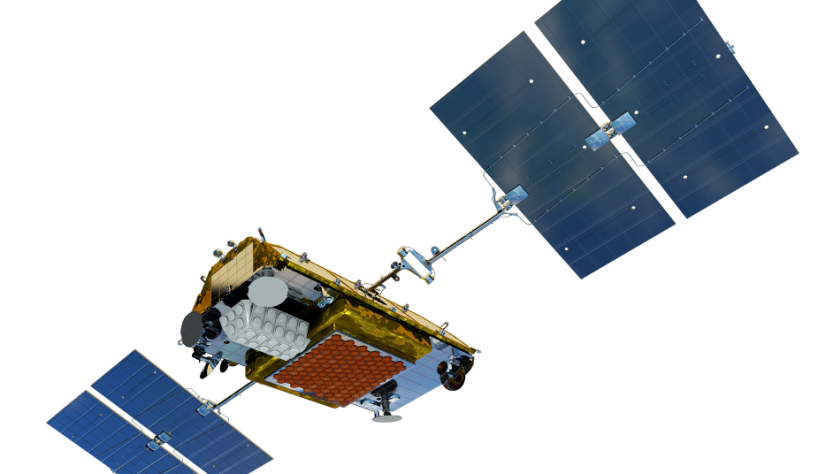
\includegraphics[width=13cm]{pic/IMG_Iridium-Satellite_NEXT-Satellite-Vehicle_HR_FEB16-clip-833x474.png}
\caption{第二代“铱星”卫星}
\label{fig:IMG_Iridium-Satellite_NEXT-Satellite-Vehicle}
\end{figure}

\begin{figure}[htbp]
\centering
\begin{minipage}[t]{0.48\textwidth}
\centering
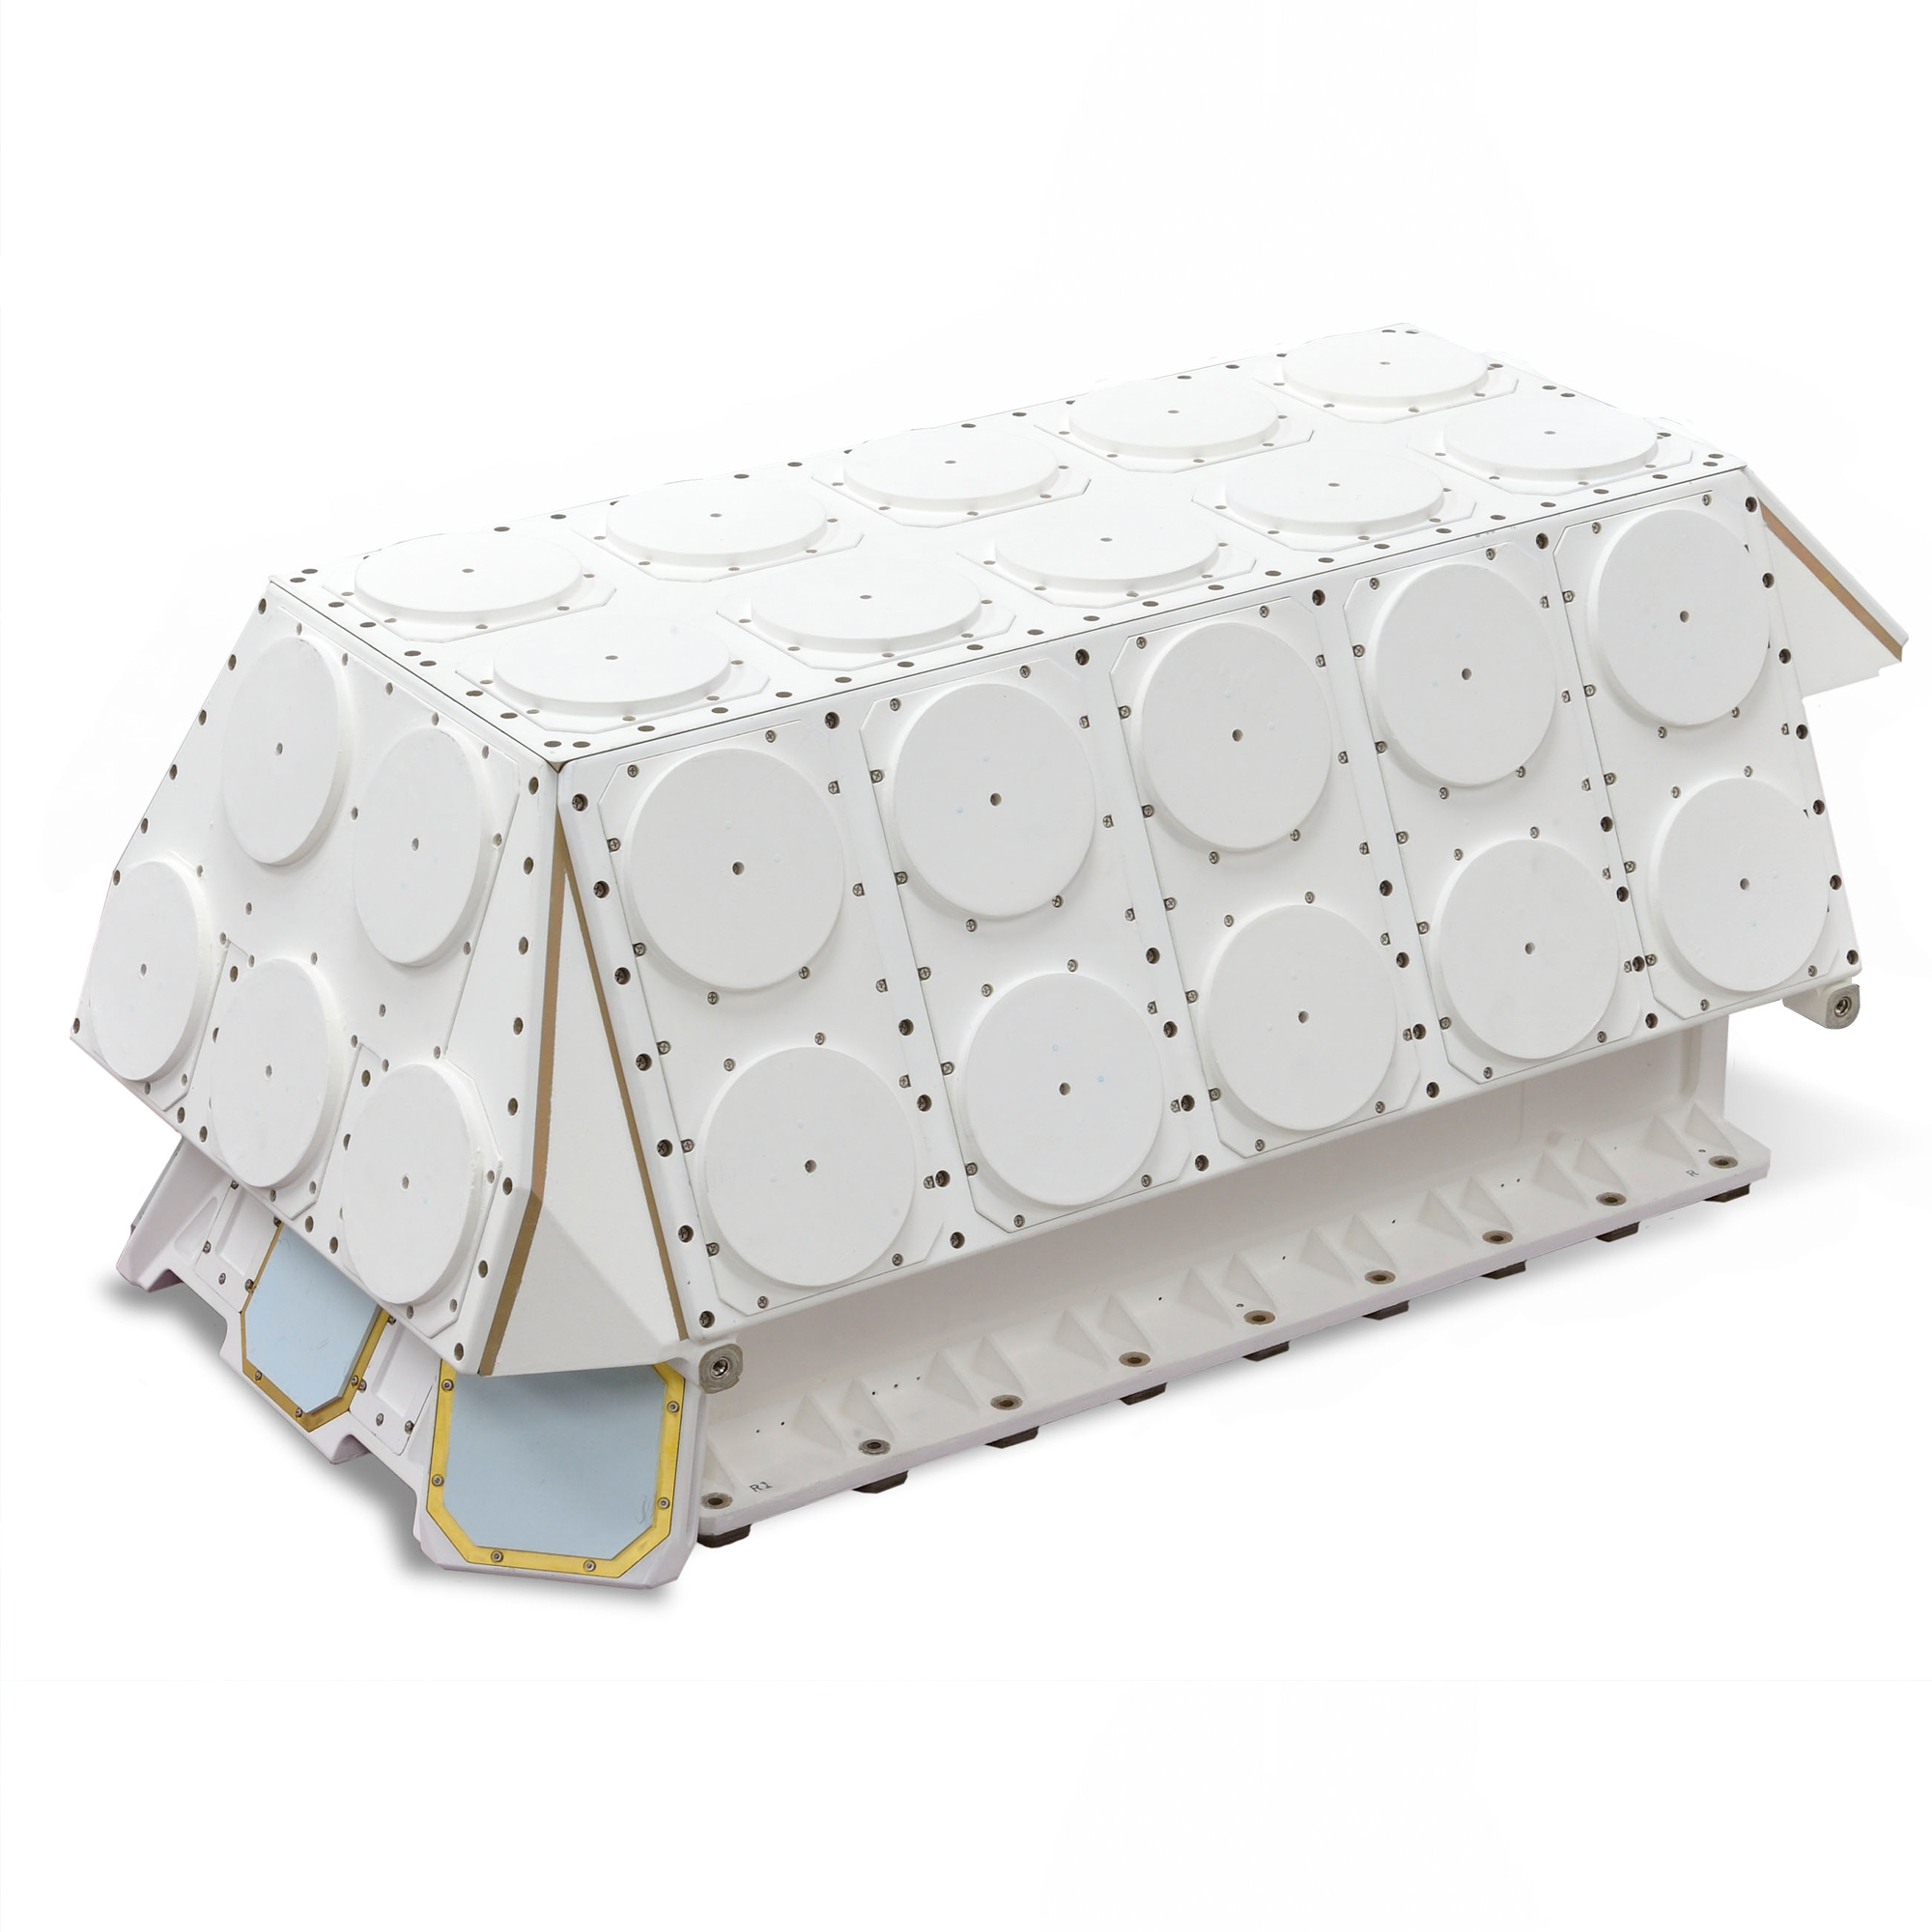
\includegraphics[width=6.5cm]{pic/Appstar_with_Base_2000x2000.jpg}
\caption{ADS-B 载荷}
\label{fig:Appstar_with_Base}
\end{minipage}
\begin{minipage}[t]{0.48\textwidth}
\centering
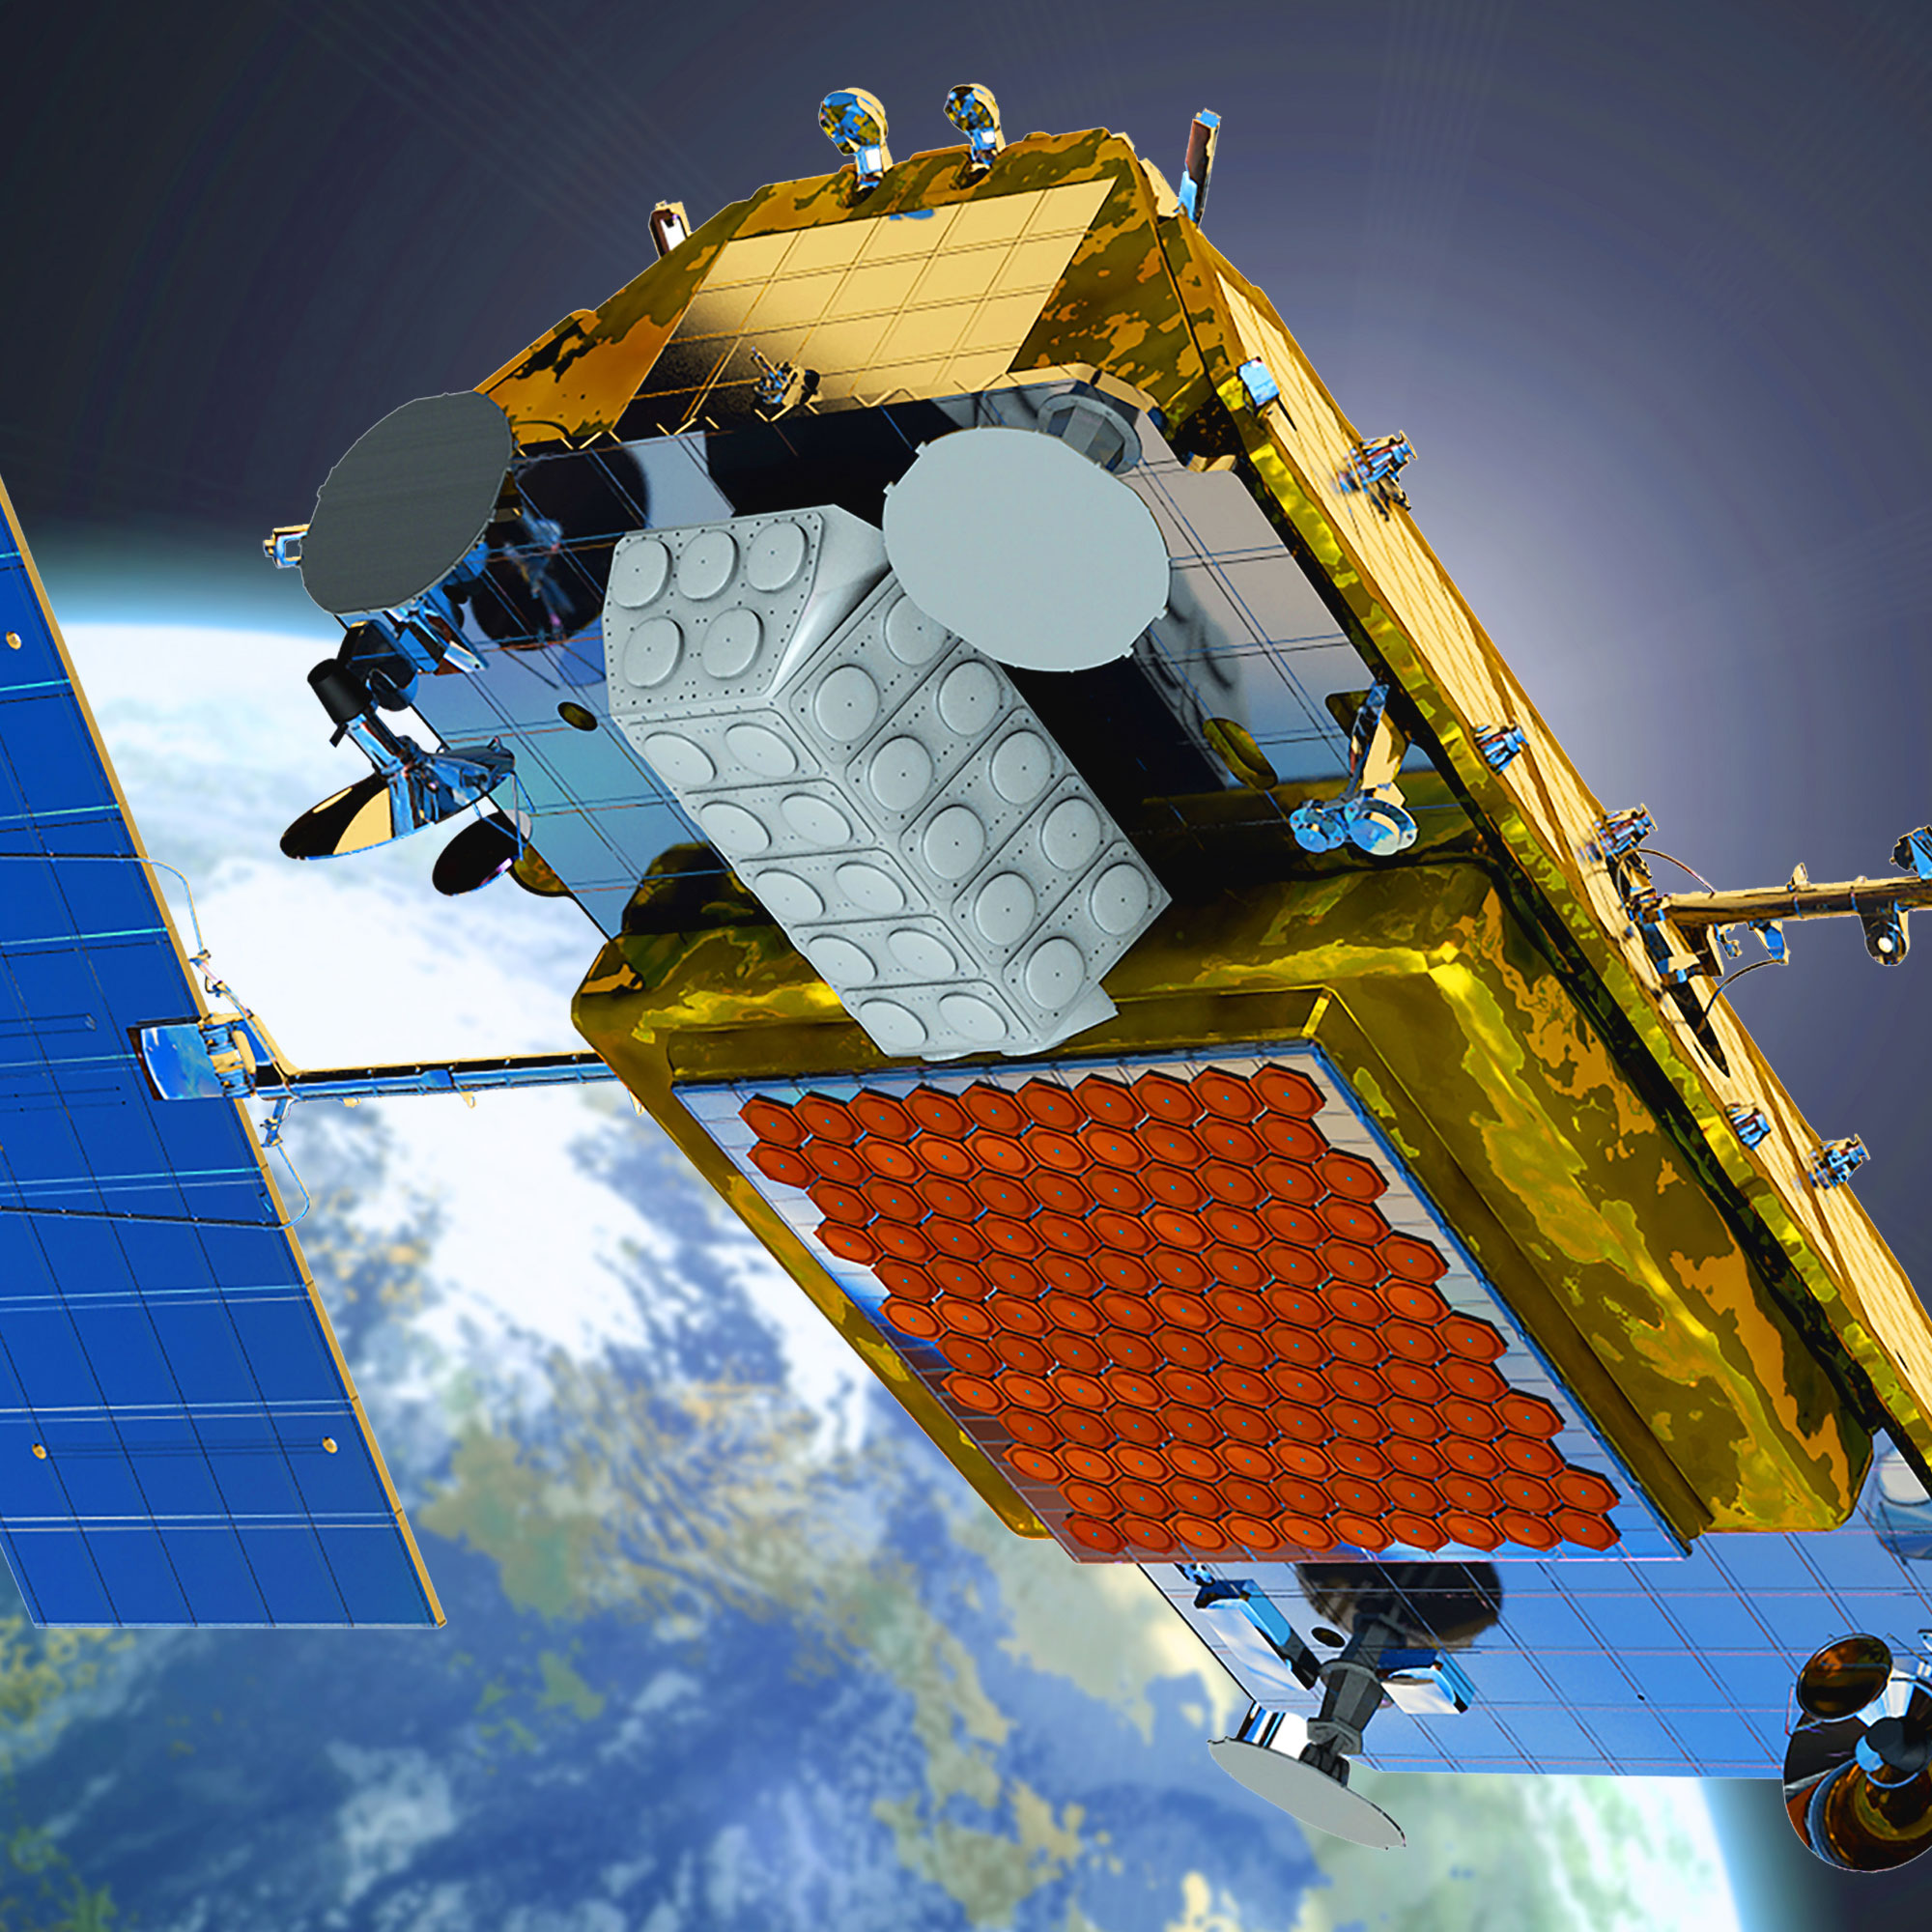
\includegraphics[width=6.5cm]{pic/reconfigurable_multimission_payloads_v2_web.jpg}
\caption{ADS-B 载荷搭载方式}
\label{fig:reconfigurable_multimission_payloads}
\end{minipage}
\end{figure}

\subsection{体系结构}

\subsection{系统性能}

\section{ALAS 系统}

\subsection{系统概述}

根据\url{www.ads-b.com}网站给出的说法,他们将天基 ADS-B 系统称为 ADS-B 链路增强系统(ADS-B Link Augmentation System),简称为“ALAS”。通过该系统,地球上任何地方的任意一架飞机可以被实时地安全追踪。

\subsection{体系结构}

\subsection{系统性能}

依托“全球星二代”系统的 ALAS 系统端到端(end-to-end)测试性能数据如表\ref{tab:alas-paras}所示。 \footnote{数据来源:\url{http://www.ads-b.com/space-based.htm}}

\renewcommand\arraystretch{1.5}
\begin{table}[htbp]
\centering
\caption{使用全球星卫星的 ALAS 系统端到端测试性能}
\label{tab:alas-paras}
\begin{tabular}[b]{|p{4cm}<{\raggedleft}|p{11cm}<{\raggedright}|}
\hline
\textbf{适用性
(Applicability)} &
ALAS 是一种简单、质量轻、低成本的外围设备,可与现有的任何 1090ES 或 UAT 电子设备配合使用,保证正常的空-地和地-空 ADS-B 传输不会中断。ALAS 还旨在与任何国家现有的 ADS-B 地面基础设施兼容\\
\hline
\textbf{覆盖范围(
Coverage Area)} &
到 2016 年,100\% 覆盖美国本土(CONUS)、GOMEX、加勒比海(Caribbean)、北大西洋(NAT)和北太平洋(NOPAC);到 2019 年,100\% 覆盖剩余地区\\
\hline
\textbf{可用性(
Availability)} & 到 2016 年,可用性为 99.99\%;到 2019 年,可用性为 99.999\% \\
\hline
\textbf{容量(
Capacity) }& 每架卫星可容纳大于 3000 架飞机(approx 1,800sm diameter)\\
\hline
\textbf{时延(
Latency)} &  从飞机到地面小于 200 毫秒;从端到端小于 300 毫秒 \\
\hline
\textbf{更新率(
Update Rate)} & 1 秒 \\
\hline
\textbf{完整性(
Integrity)} & 10E-6 \\
\hline
\textbf{精度(
Accuracy)} &
UTC 时制下,在 98\% 的时间里,相同目标的 射频视距(RF line-of-sight)导出位置和天基 ALAS 导出位置之间的显示位置差异小于 50 英尺\\
\hline
\textbf{安全性(
Security)} & 独一无二的安全。ALAS 与每架飞机建立了独特的双向连接,可以抵抗入侵、干扰或欺骗,是唯一的可以轻松加密的 ADS-B 形式。简单的防篡改设计还可以包括一个自供电备用系统,该系统将在未经授权而关闭飞机的主 ADS-B 转发器的情况下继续广播飞机的位置 \\
\hline
\textbf{可扩展性(
Scalability)}  & 高。系统架构的成本相对较低且简单,通过增加更多卫星和/或地面站,可以提高覆盖范围,可用性和容量 \\
\hline
\textbf{部署(
Deployment)} & 马上准备好。该技术已经过超过 100 小时的飞行测试。Globalstar 在过去两年中发射了 24 颗新的第二代 ALAS 卫星。Essential Services could be deployed as early as 3Q2016 and Critical Services NLT 2019\\
\hline
\textbf{成本(
Cost)} & 低。由于 ALAS 不需要新的卫星或太空中的其他技术,因此 ANSP 的买入和重复成本很小。它还可以与现有的 ADS-B 地面基础设施轻松连接。The price point for Part 121 avionics is less than \$40k and installation should be in the 20-25 MH range for most commercial aircraft. \\
\hline
\end{tabular}

\end{table}

% !TEX root = ../document.tex

\chapter{系统面临的挑战}

\section{覆盖范围}

\begin{enumerate}
    \item 由于信号相关性差,1090MHz S 模式格式不适用于接收弱信号(<-90dBm)
    \item 飞机与 LEO 卫星之间的距离约为 800 公里(444 海里)
    \item 1090ES ADS-B 的“正常”覆盖范围为:50NM A/A,150NM A/G
\end{enumerate}

\section{调制方案}

脉冲位置调制(PPM)不适合对噪声水平附近的信号进行解码

\section{报文冲突}

\begin{enumerate}
    \item 由于接收位置高,覆盖范围广
    \item 加上随机通道访问 $\geq$ ADS-B报告的重叠
    \item 使用波束天线的补偿措施:空间选择性 + 天线增益
\end{enumerate}

\section{静锥区}

飞机应答器天线垂直天线的凹陷

% !TEX root = ../document.tex

\chapter{系统发展展望}

% !TEX root = ../document.tex

\begin{thebibliography}{99}

\bibitem{z1}王洪全,刘天华,欧阳承曦,姚待艳.基于星基的ADS-B系统现状及发展建议[J].通信技术,2017,50(11):2483-2489.

\bibitem{z2}

\bibitem{z3}

\bibitem{z4}

\bibitem{e1} Ali, Syd B . System specifications for developing an Automatic Dependent Surveillance-Broadcast (ADS-B) monitoring system[J]. International Journal of Critical Infrastructure Protection, 2016:S187454821530041X.

\bibitem{e2} K. Werner . ADS-B over Satellite The world’s first ADS-B receiver in Space.

\bibitem{e3} Kunzi F , Hansman R J . ADS-B Benefits to General Aviation and Barriers to Implementation[J]. Massachusetts Institute of Technology, 2011.

\bibitem{e4} Wang, Hao, "ADS-B used in Improvement of Air Traffic Control" (2015). Open Access Theses. 624.
\url{https://docs.lib.purdue.edu/open_access_theses/624}

\bibitem{e5} SESAR, ADS-B and other means of surveillance implementation status

\bibitem{e6} ADS-B SITF/15 – IP/31, UPDATE ON ADS-B ACTIVITIES IN CHINA

\bibitem{e7} SEA/BOB ADS-B WG/14 – IP/3, ADS-B IMPLEMENTATION ACTIVITIES IN CHINA

\bibitem{e8} ADS-B SITF/14 – IP/23 (Rev.), ADS-B IMPLEMENTATION STATUS IN INDONESIA AND DATA SHARING BETWEEN INDONESIA, AUSTRALIA AND SINGAPORE

\bibitem{e9} SEA/BOB ADS-B WG/13 – IP/09, UPDATE ON ADS-B PROJECT IN MALAYSIA

\bibitem{e10} SEA/BOB ADS-B WG/12 – IP/09, UPDATE ON ADS-B IMPLEMENTATION IN THAILAND

\bibitem{e11} SEA/BOB ADS-B WG/13 – IP/17, UPDATE ON ADS-B IMPLEMENTATION IN THE PHILIPPINES

\bibitem{e12}

\bibitem{e13}

\bibitem{h1}“What is Space-Based ADS-B?”,\url{http://www.ads-b.com/space-based.htm}

\bibitem{h2}“ADS-B over Satellite”,\url{https://directory.eoportal.org/web/eoportal/satellite-missions/a/ads-b#overview}

\bibitem{h3}“Iridium satellite constellation”,\url{https://en.wikipedia.org/wiki/Iridium_satellite_constellation#Next-generation_constellation}

\bibitem{h4}“铱星系统的前世今生,通导融合的技术奇迹”,\url{http://mini.eastday.com/mobile/170228225143989.html#}

\bibitem{h5}“看‘铱星二代’和‘全球星二代’两个‘星二代’是如何当航空监视‘保镖’的?”,\url{http://www.sohu.com/a/211117337_100044418}

\bibitem{h6}“Aireon, SPACE-BASED ADS-B MAKING GLOBAL AIR TRAFFIC SURVEILLANCE A POWERFUL REALITY”,\url{https://aireon.com/}

\bibitem{h7}“WHERE IS ADS-B OUT REQUIRED?”,\url{https://www.aopa.org/go-fly/aircraft-and-ownership/ads-b/where-is-ads-b-out-required}

\bibitem{h8}“What is VDL Mode 4?”,\url{http://www.cns.se/support/faq-vdl_mode_4}

\bibitem{h9}

\bibitem{h10}

\end{thebibliography}

\end{document}
